\documentclass[a4paper]{article}

%% Language and font encodings
\usepackage[english]{babel}
\usepackage[utf8x]{inputenc}
\usepackage[T1]{fontenc}

%% Sets page size and margins
\usepackage[a4paper,top=3cm,bottom=2cm,left=3cm,right=3cm,marginparwidth=1.75cm]{geometry}

%% Useful packages
\usepackage{amsmath, amssymb}
\usepackage{bm}
\usepackage{graphicx}
\usepackage[colorinlistoftodos]{todonotes}
\usepackage[colorlinks=true, allcolors=blue]{hyperref}
\usepackage{array}
\usepackage{multirow}
\usepackage{svg}
\usepackage{makecell}

\graphicspath{{./img/}}

\title{Information Theory Through Toy Examples}
\author{Matthew Andres moreno}

\begin{document}
\maketitle

\section{Motivation}
Clean the gutters, clear enough space in the garage to park the car, organize a laundry bin of family photos, respond to an email that's been wallowing too long at the bottom of the inbox\ldots we all have a list of things we've been meaning to get around to.
Learning a bit of information theory has been one of those things I meant to get around to for longer than I would like to admit.
A few weeks ago, I ran into Dr. Chris Adami at the BEACON Congress.
He recommended a pair of introductory papers on information theory.
In \cite{Adami2016}, he provides a lively introduction to information theory that pays special attention to guiding newcomers through commonly-encountered intellectual obstacles and dispelling common misconceptions about information theory.
In \cite{Adami2012}, Adami presents an information theoretic perspective on genetic material and brains, ultimately demonstrating how these substrates fundamentally promote fitness by allowing organisms to exploit information about their environments.

With these papers on my desk, it was finally time to learn a little information theory.
Now that I've spent a few hours brushing up on it, I'm glad to have this new addition to my scientific toolbelt.
I found the papers Dr. Adami recommended to be accessible and useful.
I really had my lightbulb moment, though, when I took a little time to cook up some toy examples and walk through the math on my own.
I'd like to share them with you here.
There will be a little math along the way, but it is just in service of the toy stories I want to tell.
what I found most valuable about this exercise when I worked through it on my own was seeing how the results of the math tie in to the story.
So, don't let the math spook you.
The math is just in service of the story.
Ultimately, I hope these examples might strike a first spark of intuition, or at least serve as an invitation to dip a toe into information theory.


\section{Introduction}

We must start out by defining \textit{entropy}.
Entropy is kind of a fancy word for uncertainty.
My past encounters with the word entropy have been mostly confusing, verging on mystical.
I'm sure many of us have been told, ``the entropy of the universe is always increasing.''
Let's leave entropy's existential baggage behind and treat it just like any other run-of-the-mill word.
The best way to get a practical feel for entropy is with an example.

We have a coin.
The coin has a red side and a grey side.
\begin{center}
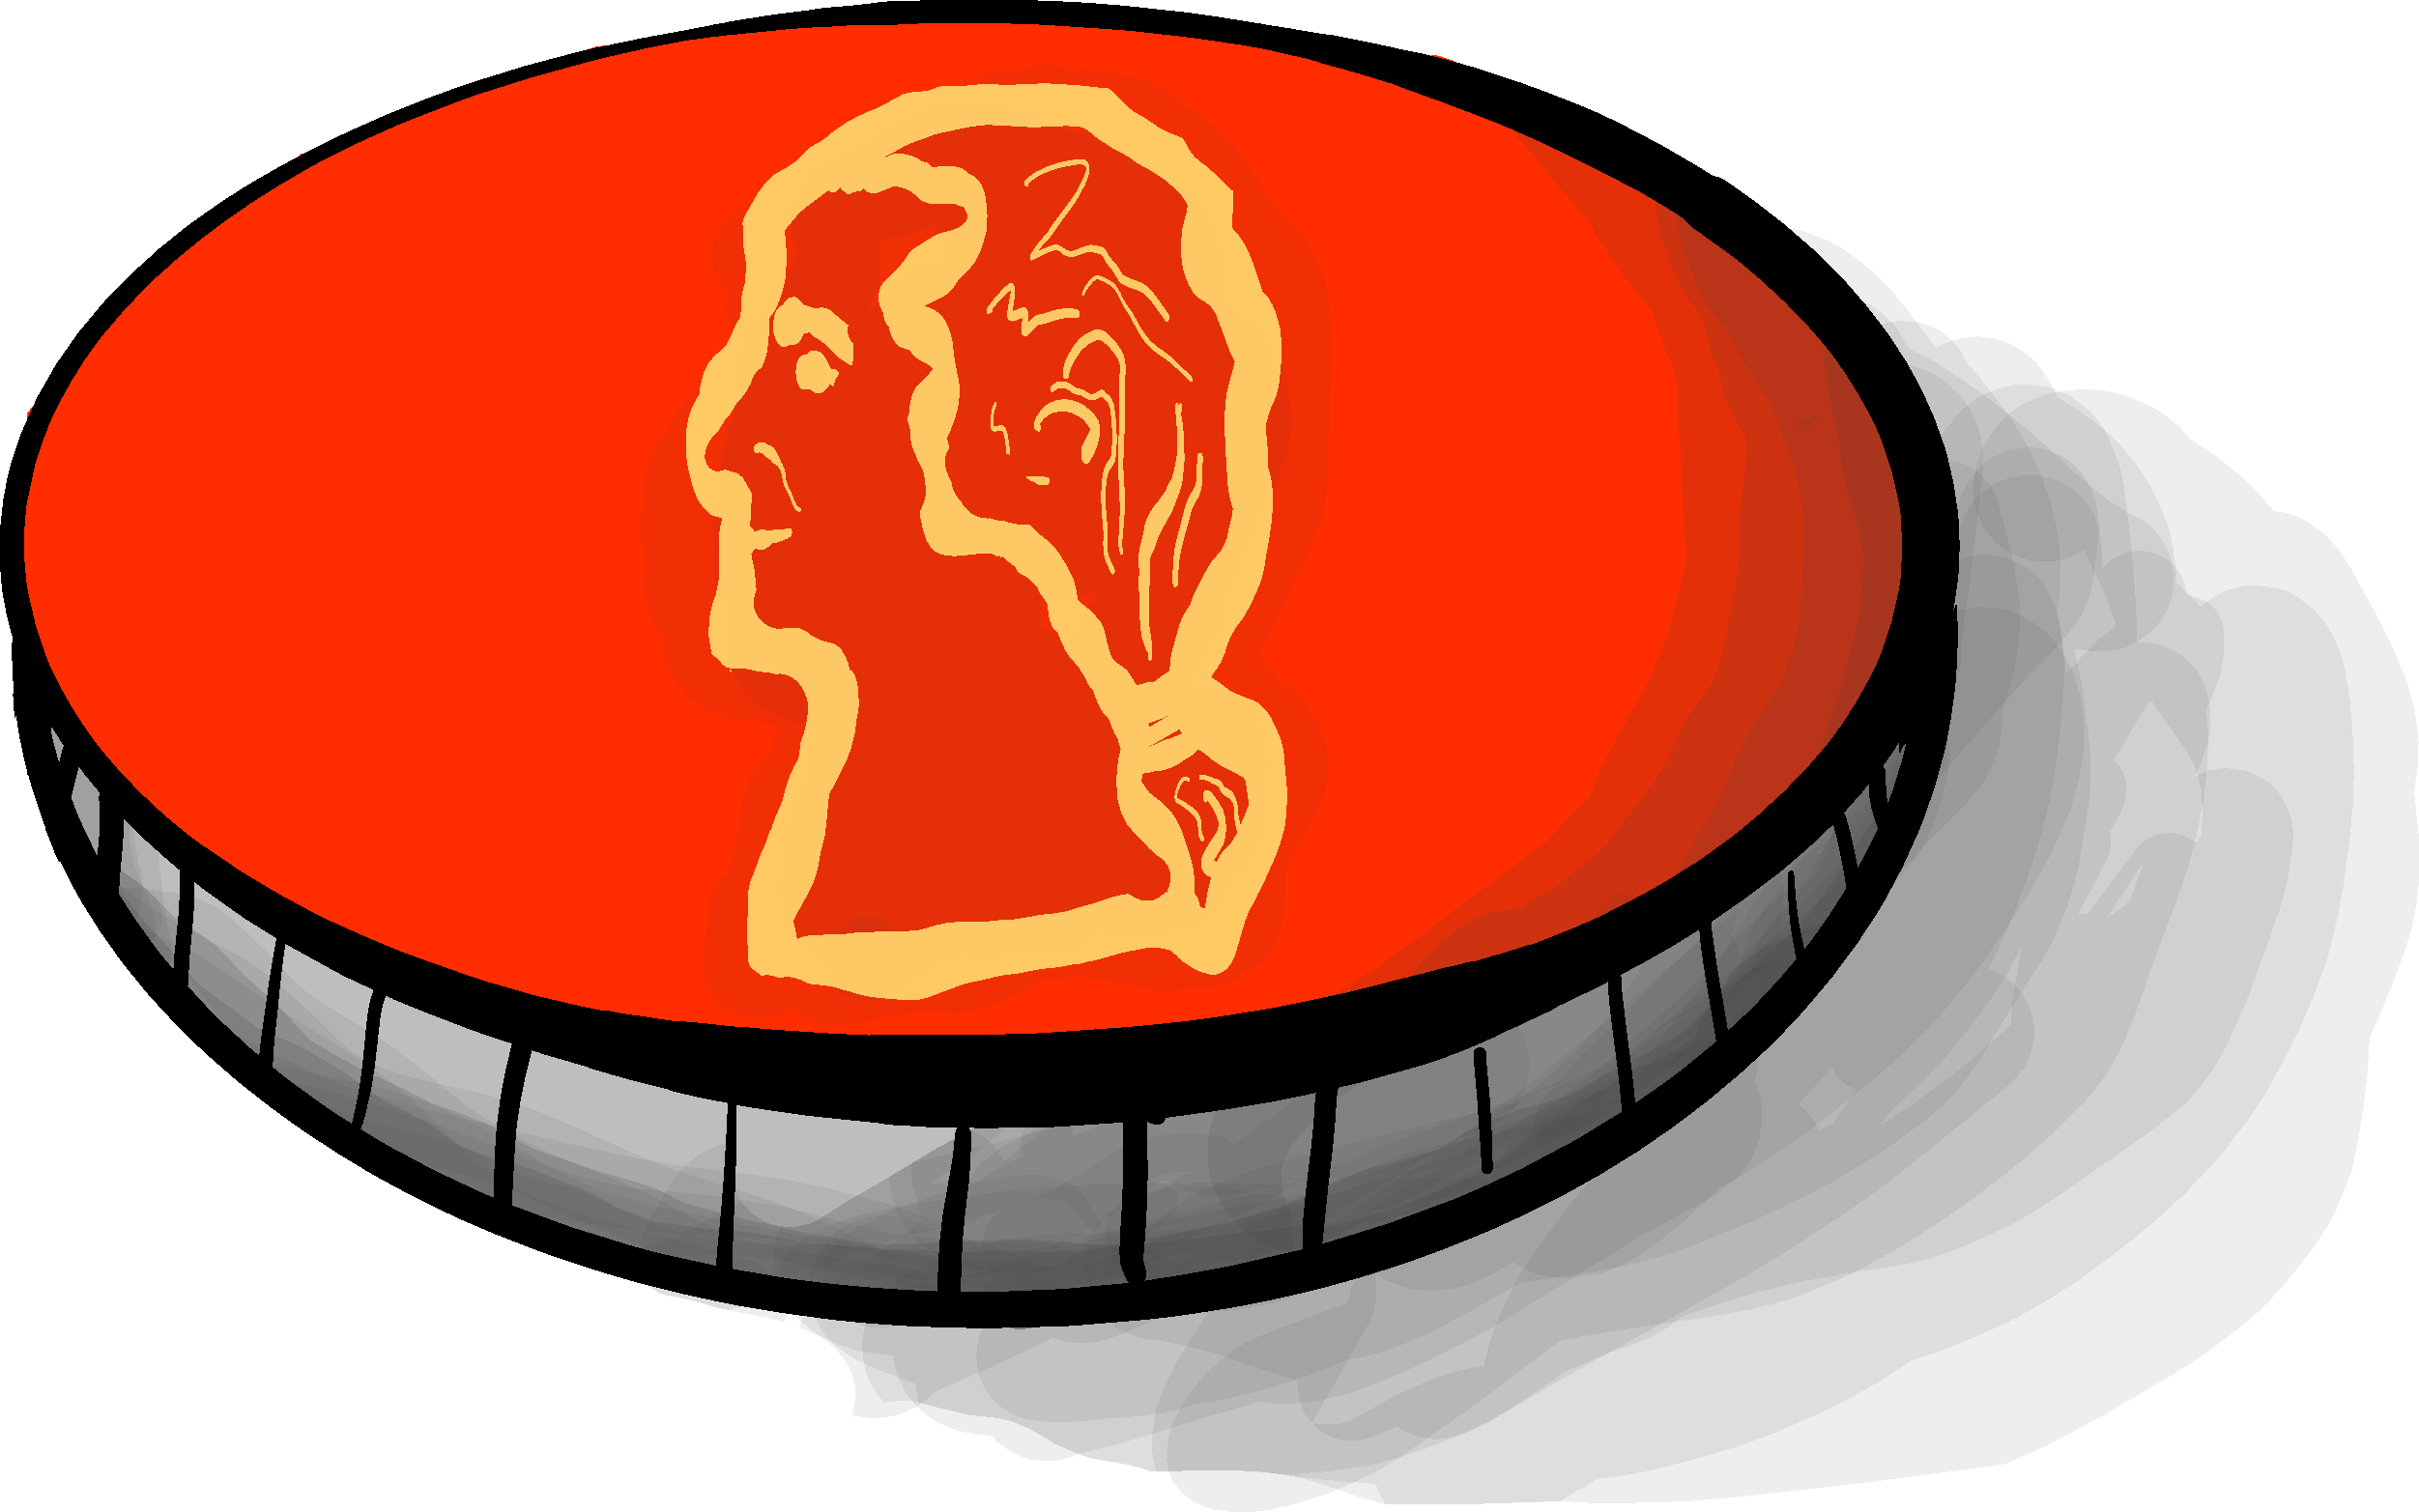
\includegraphics[width=0.3\textwidth]{img/red-coin}
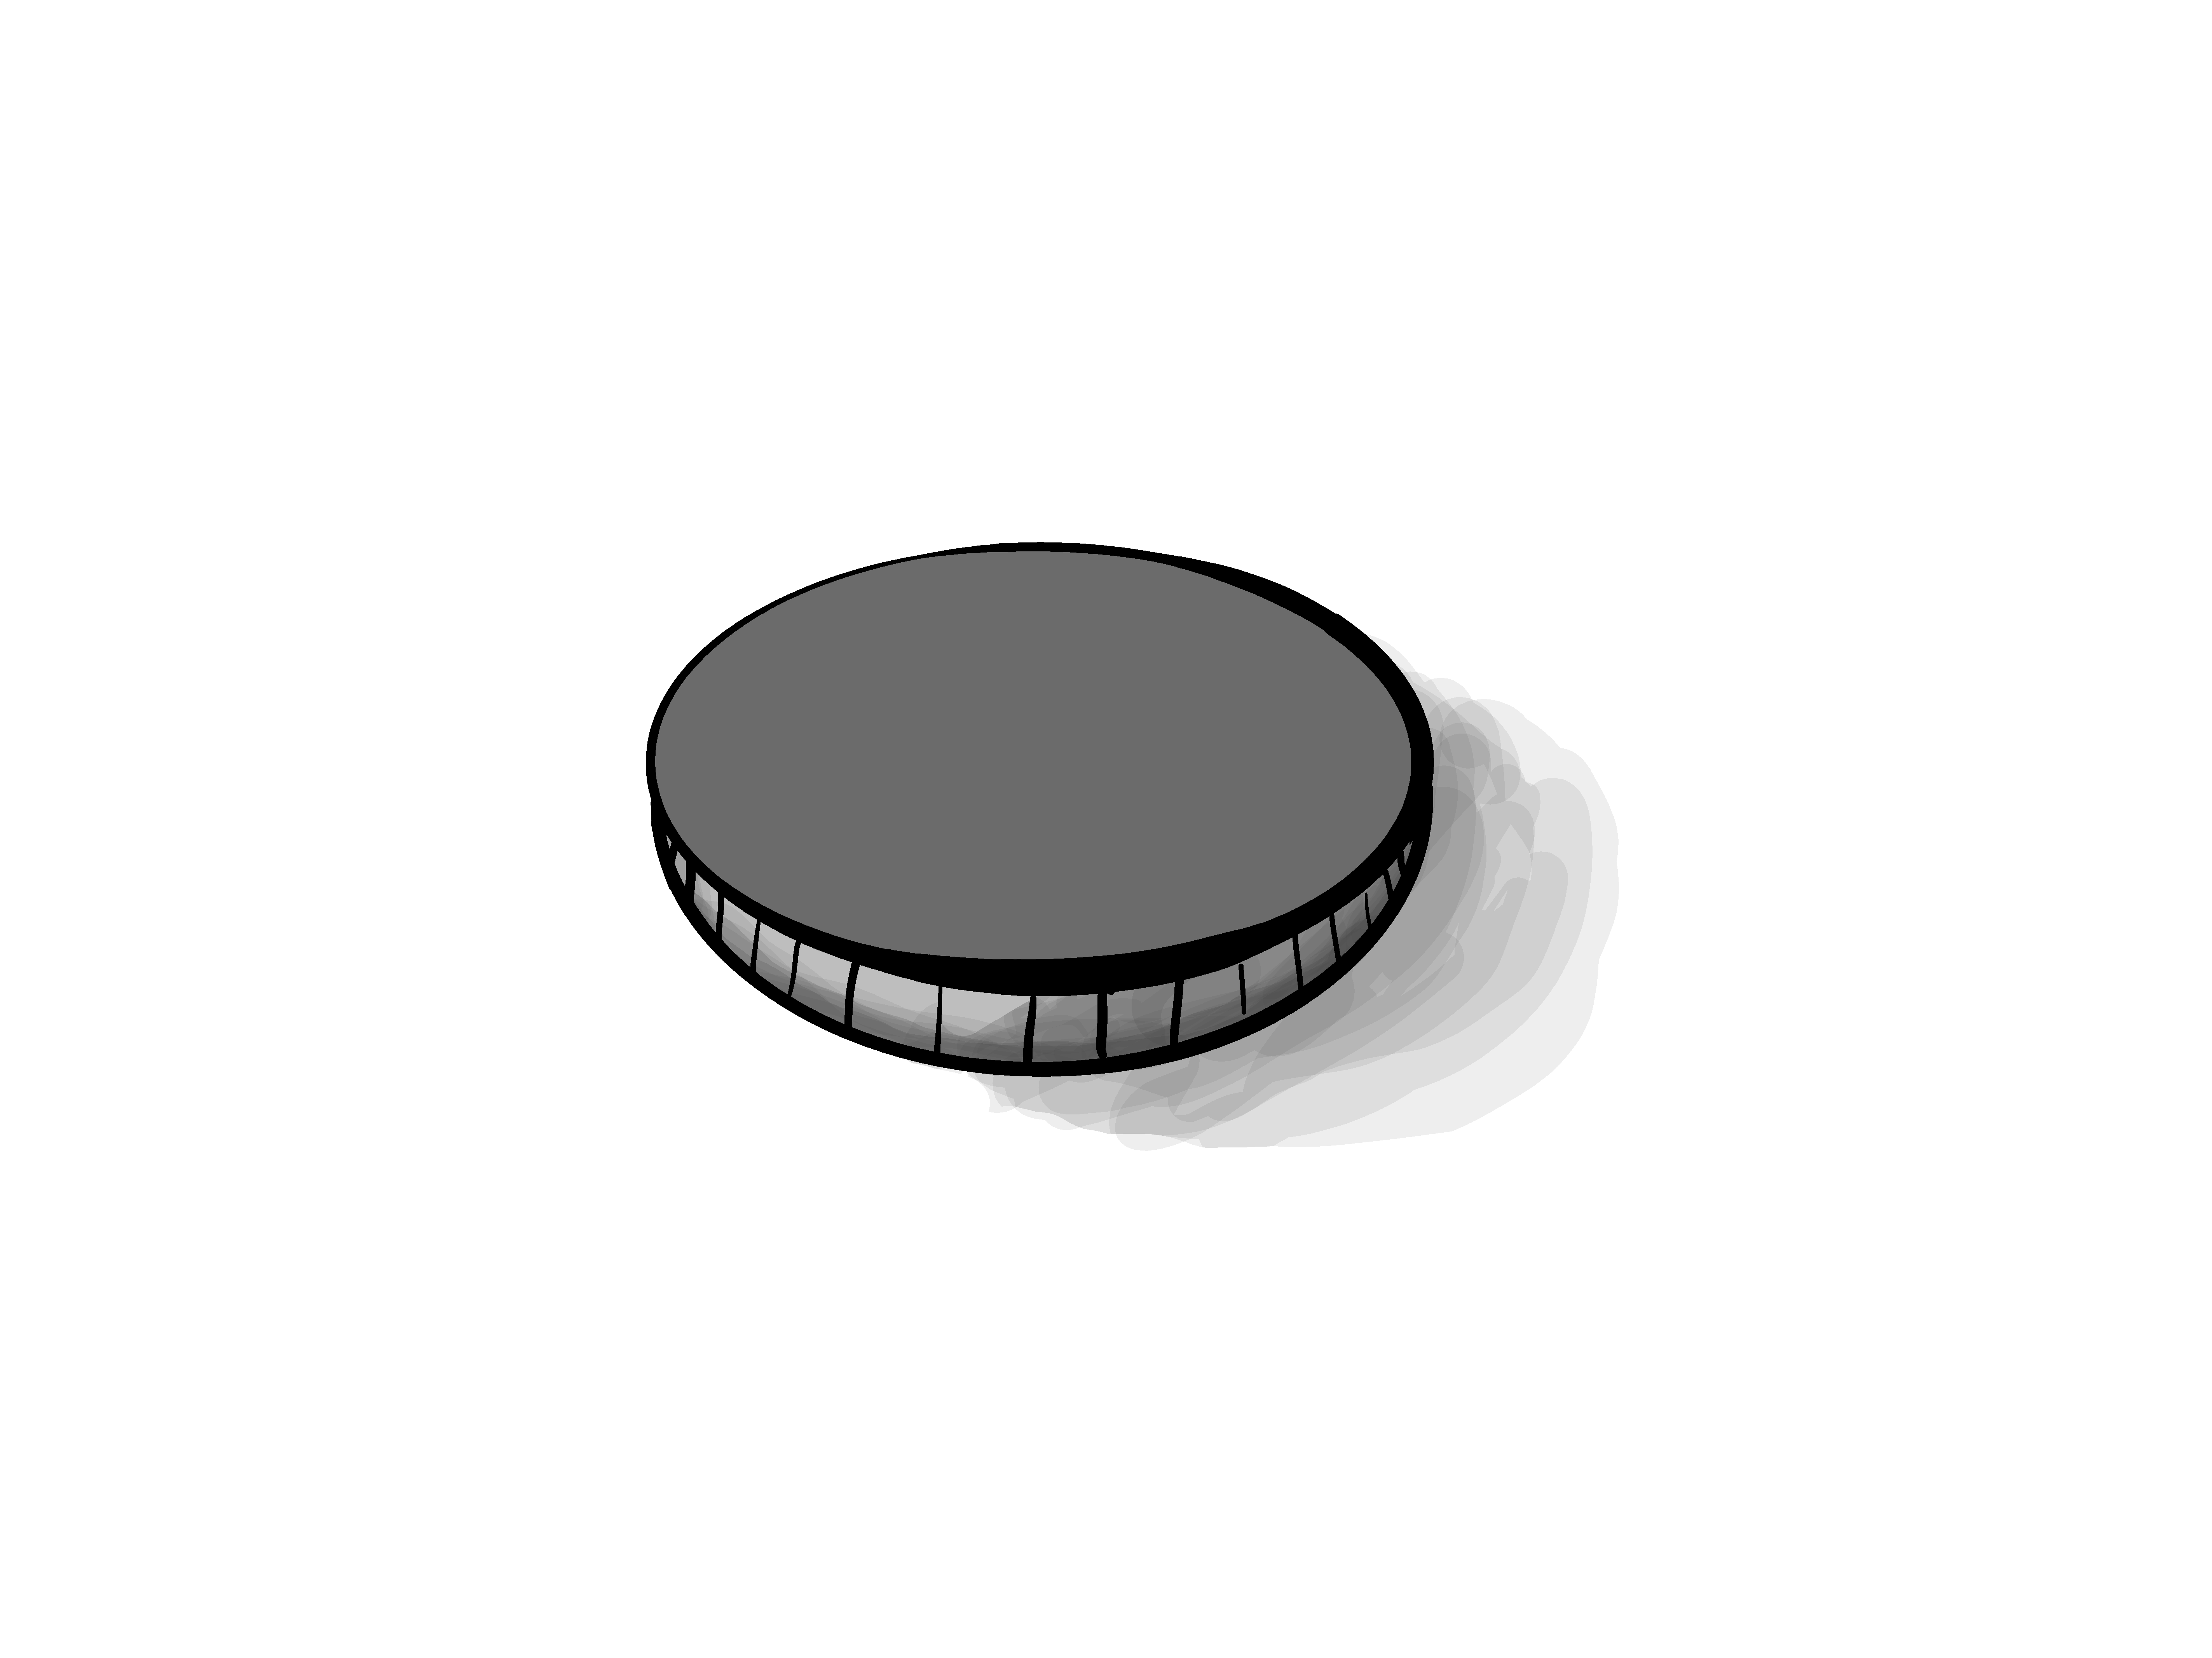
\includegraphics[width=0.3\textwidth]{img/grey-coin}
\end{center}
The coin is evenly weighted so if we were to throw it in the air, half of the time it would land red side up and the other half of the time it would land grey side up.
If we model our coin as a random variable $\bm{C}$, we can write this mathematically as $p_{\bm{C} = \text{red}} = 0.5$ and $p_{\bm{C} = \text{grey}} = 0.5$.

Let's put the coin in a box.
\begin{center}
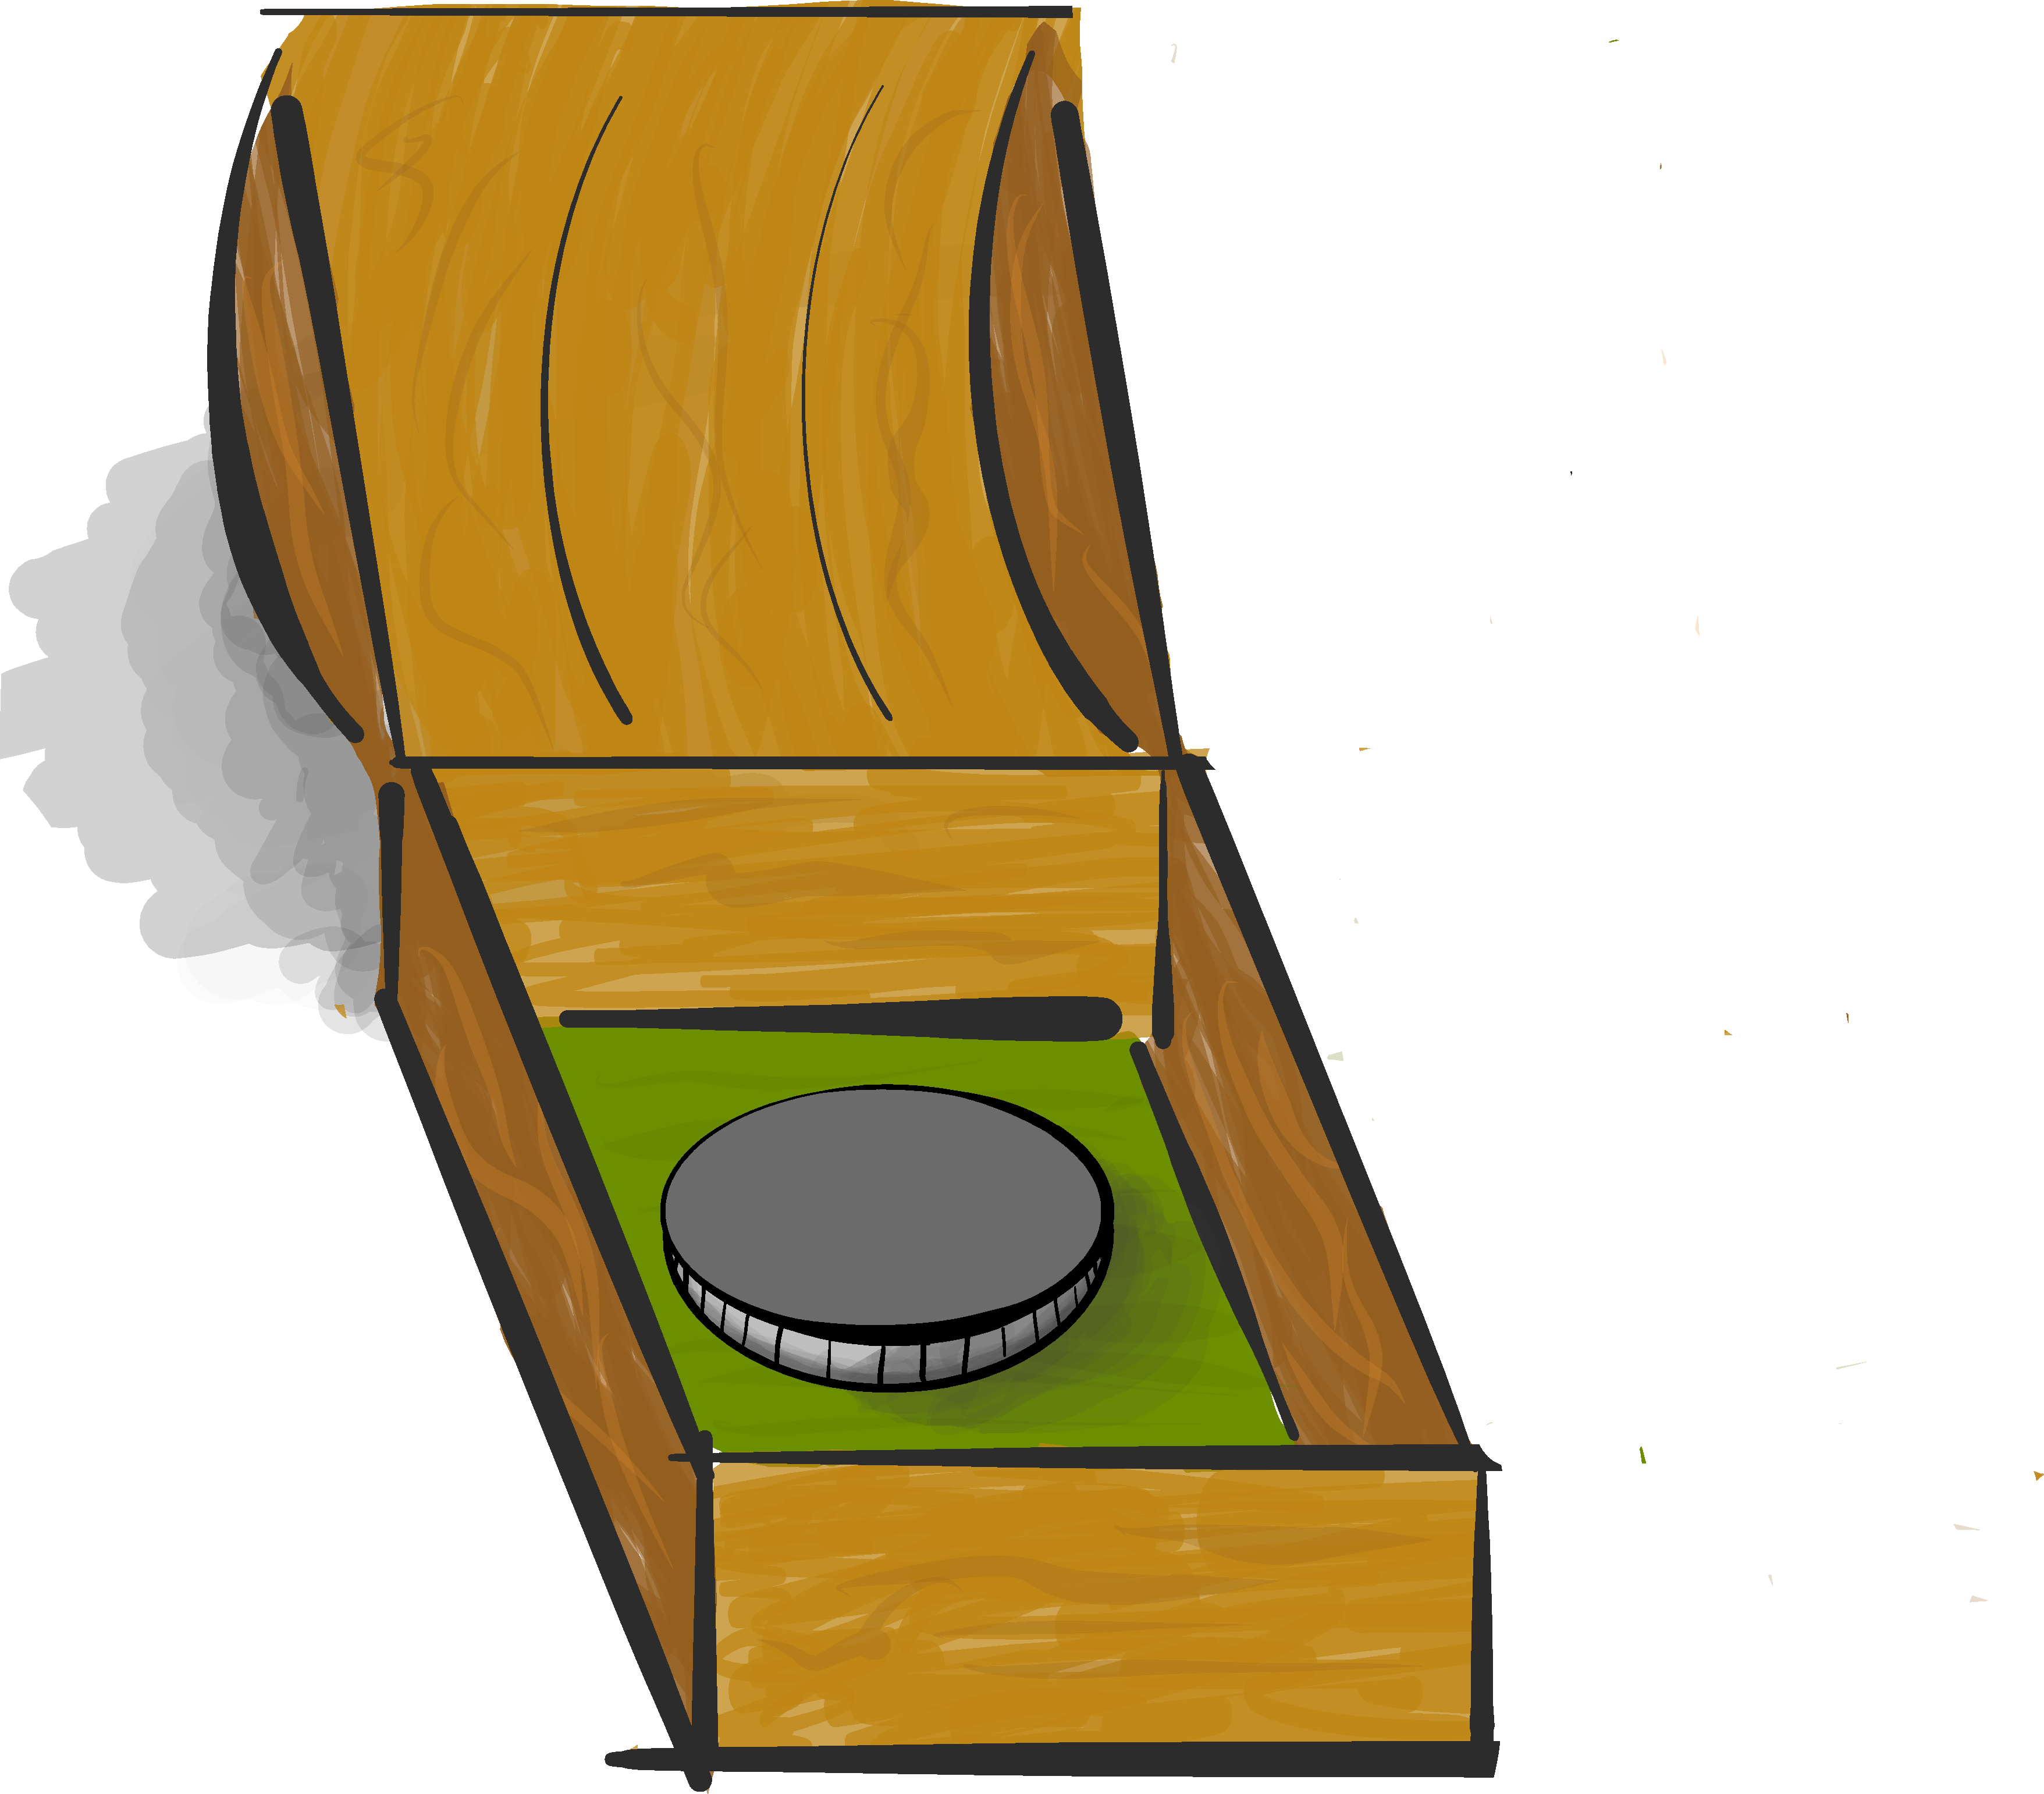
\includegraphics[width=0.3\textwidth]{img/big-box-open-coin}
\end{center}
Right now, the grey side of the coin is facing up.
How much uncertainty do we have in regard to the position of the coin?
None.
We know the grey side of the coin is facing up.
Thus, entropy is zero.
To say this mathematically, we write $S = 0$.

What about the entropy of the molecules that make up the coin?
What about the entropy of the universe?
We don't have to worry about any of that.
Entropy has no intrinsic meaning.
It's just a tool that we use to help us concretely understand a particular situation.
Right now we are just thinking about which way a coin is facing.
So, right now entropy just describes our uncertainty about which way that coin is facing.

Let's close the box and give it a good shake.
\begin{center}
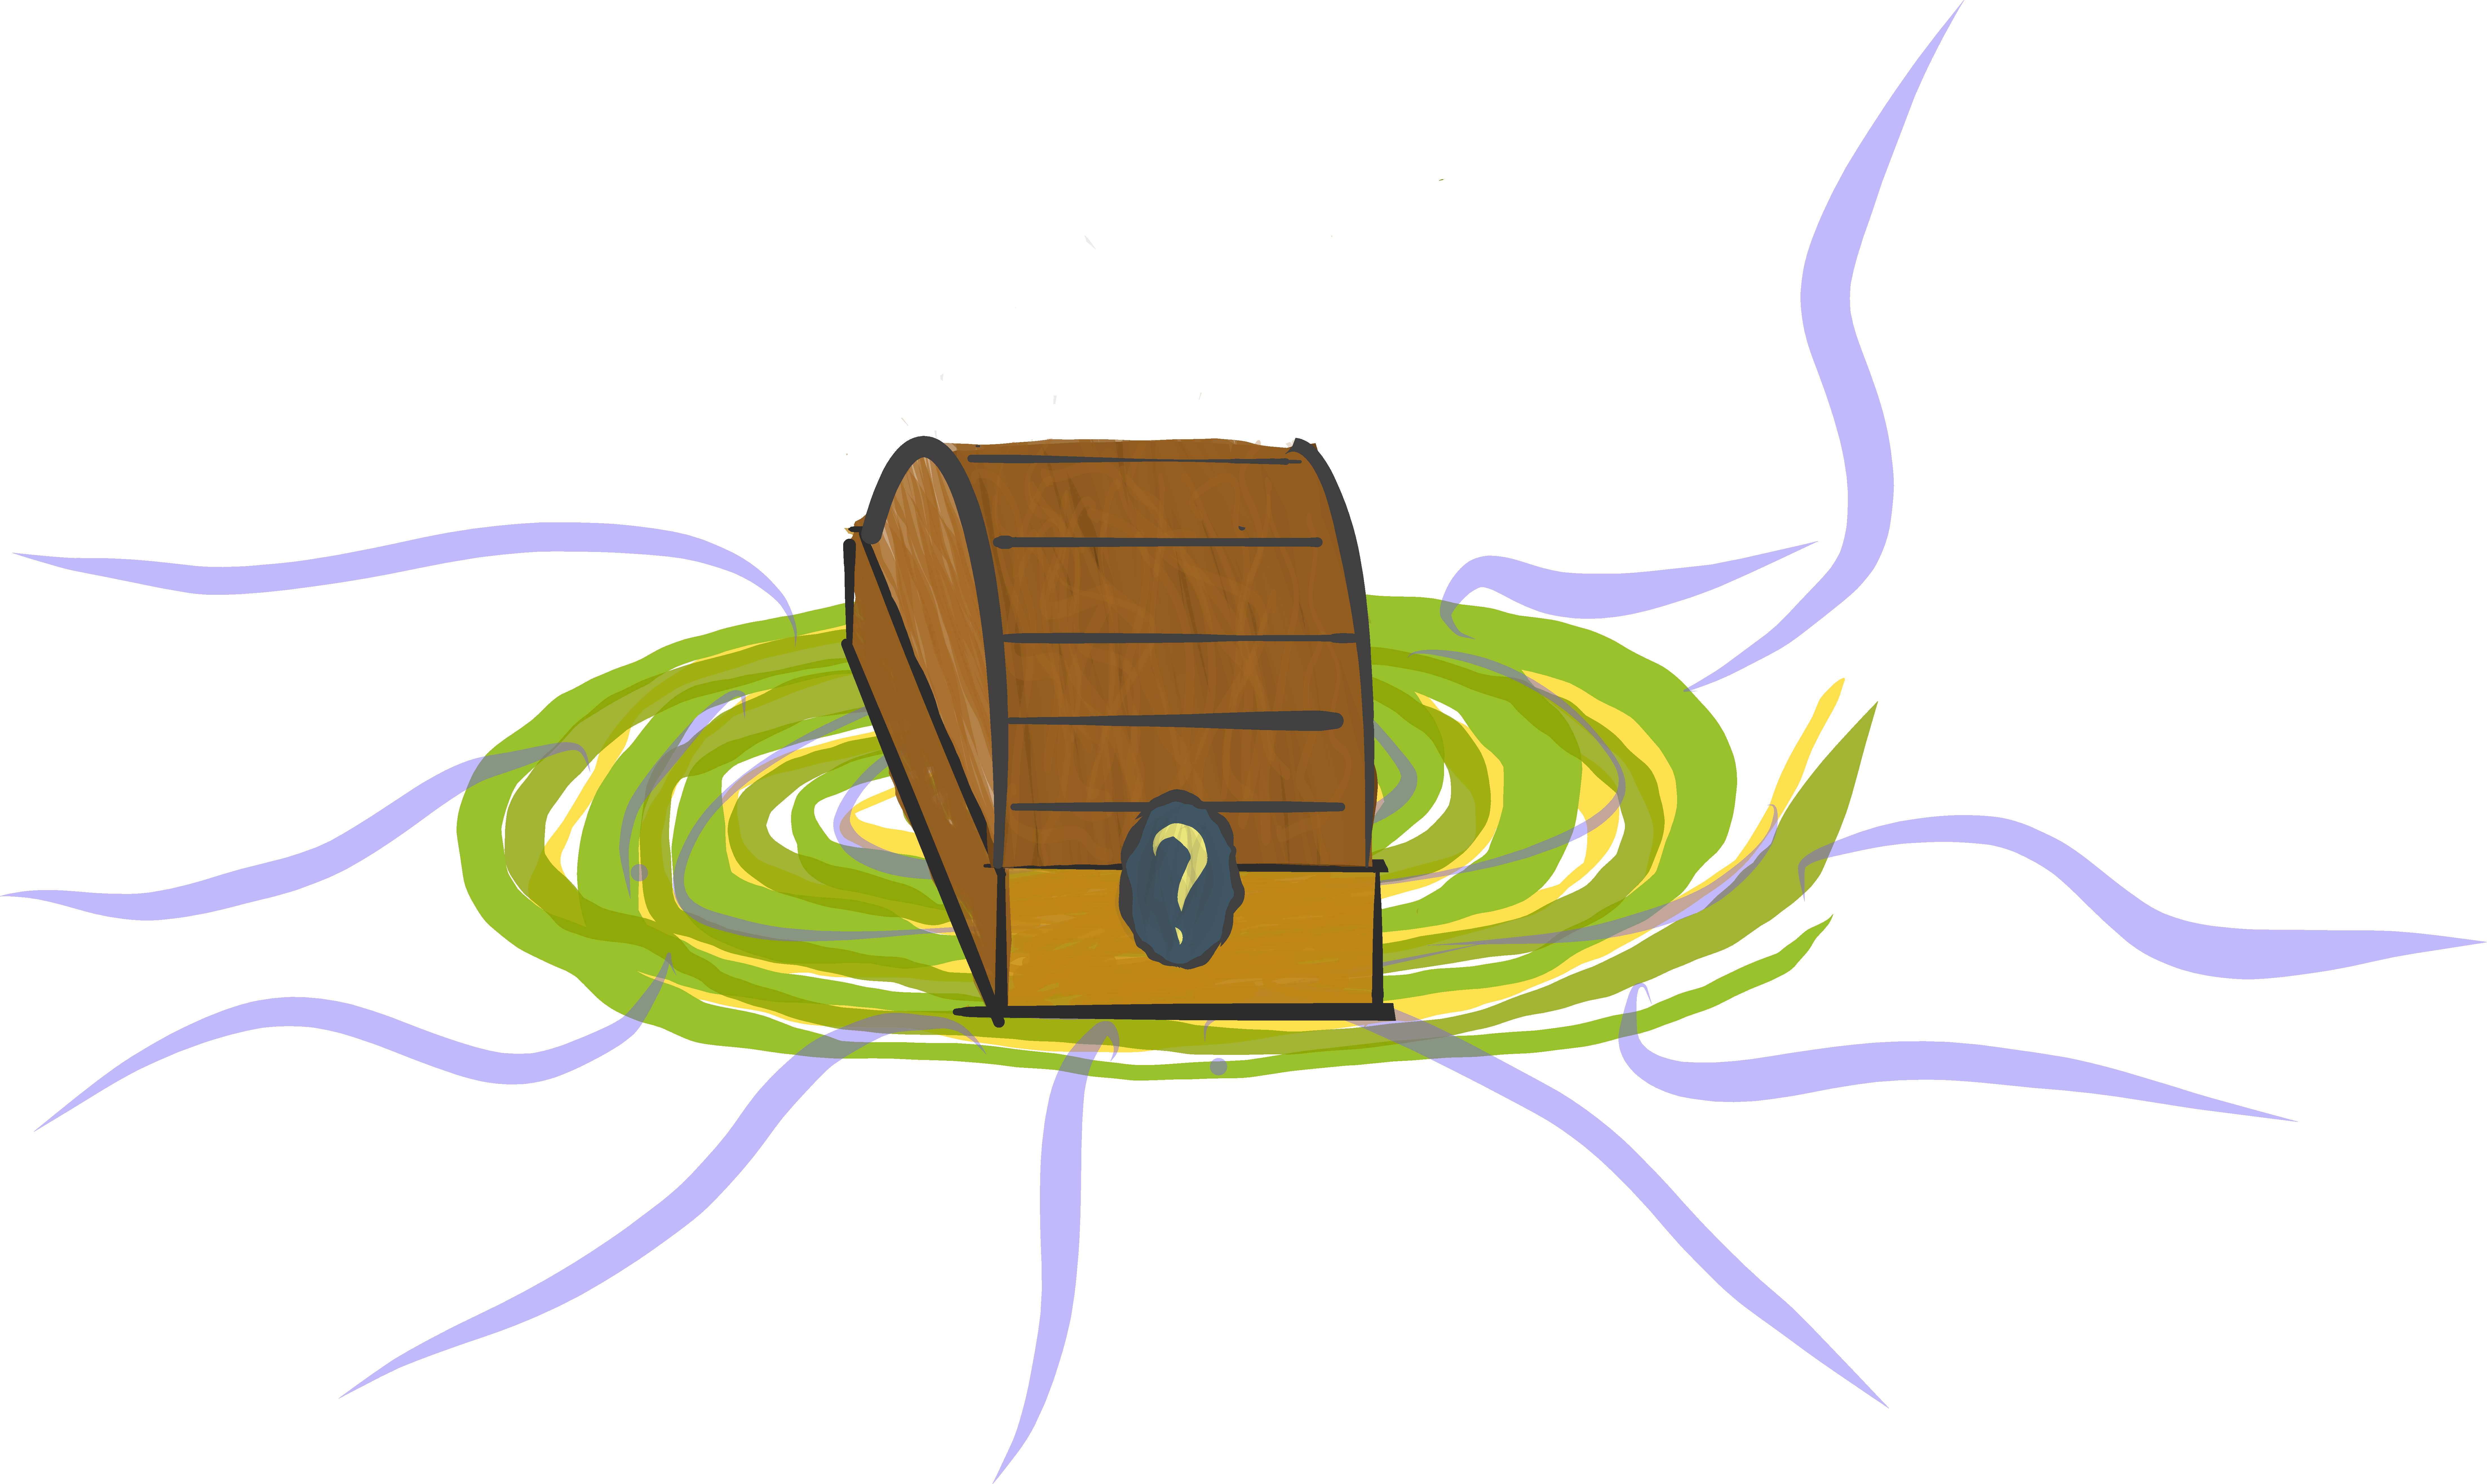
\includegraphics[width=0.7\textwidth]{img/big-box-closed-portal}
\end{center}
We're no longer certain of the coin's position.
So, the entropy is greater than zero, or $S > 0$.
We can use Shannon's equation to make a more specific mathematical statement about the entropy of our coin.

In general, Shannon's equation allows us to use the set of probabilities for possible outcomes from a random variable $\{p_1, p_2, \ldots, p_n\}$ to calculate the entropy of that random variable $\bm{X}$.
The equation looks like this,
\begin{align} \label{eqn:shannon}
S
&= H(\bm{X}) \\
&= \sum_{i=1}^{n} -p_i \log(p_i)
\end{align}
This equation is the main tool we'll use to work through our toy examples.
If you're curious about the intuition behind its mathematical form, check out \cite{Adami2016}.

Recall that for our coin, $\{p_{\text{red}} = 0.5, p_{\text{grey}} = 0.5 \}$.
Plugging and chugging with Equation \ref{eqn:shannon}, we calculate
\begin{align*}
S_{\text{coin}}
&= H(\bm{C}) \\
&= -0.5 \log(0.5) + -0.5 \log(0.5) \\
&= 1.
\end{align*}
We used the base two logarithm to perform this calculation, so the unit that describes our entropy value is the ``bit.''
(For those unfamiliar, bit refers to a binary value, one that may only take one of two possible states: a one or a zero.
The bit is the appropriate unit for the entropy value because the base of our logarithm matches the number of possible states of a bit.)
For consistency's sake, we will use the base two logarithm and the bit unit for all the rest of the calculations we perform.
Thus, we say that the coin closed in the box has one bit of entropy.

Now, let's open the box and observe the state of the coin.
\begin{center}
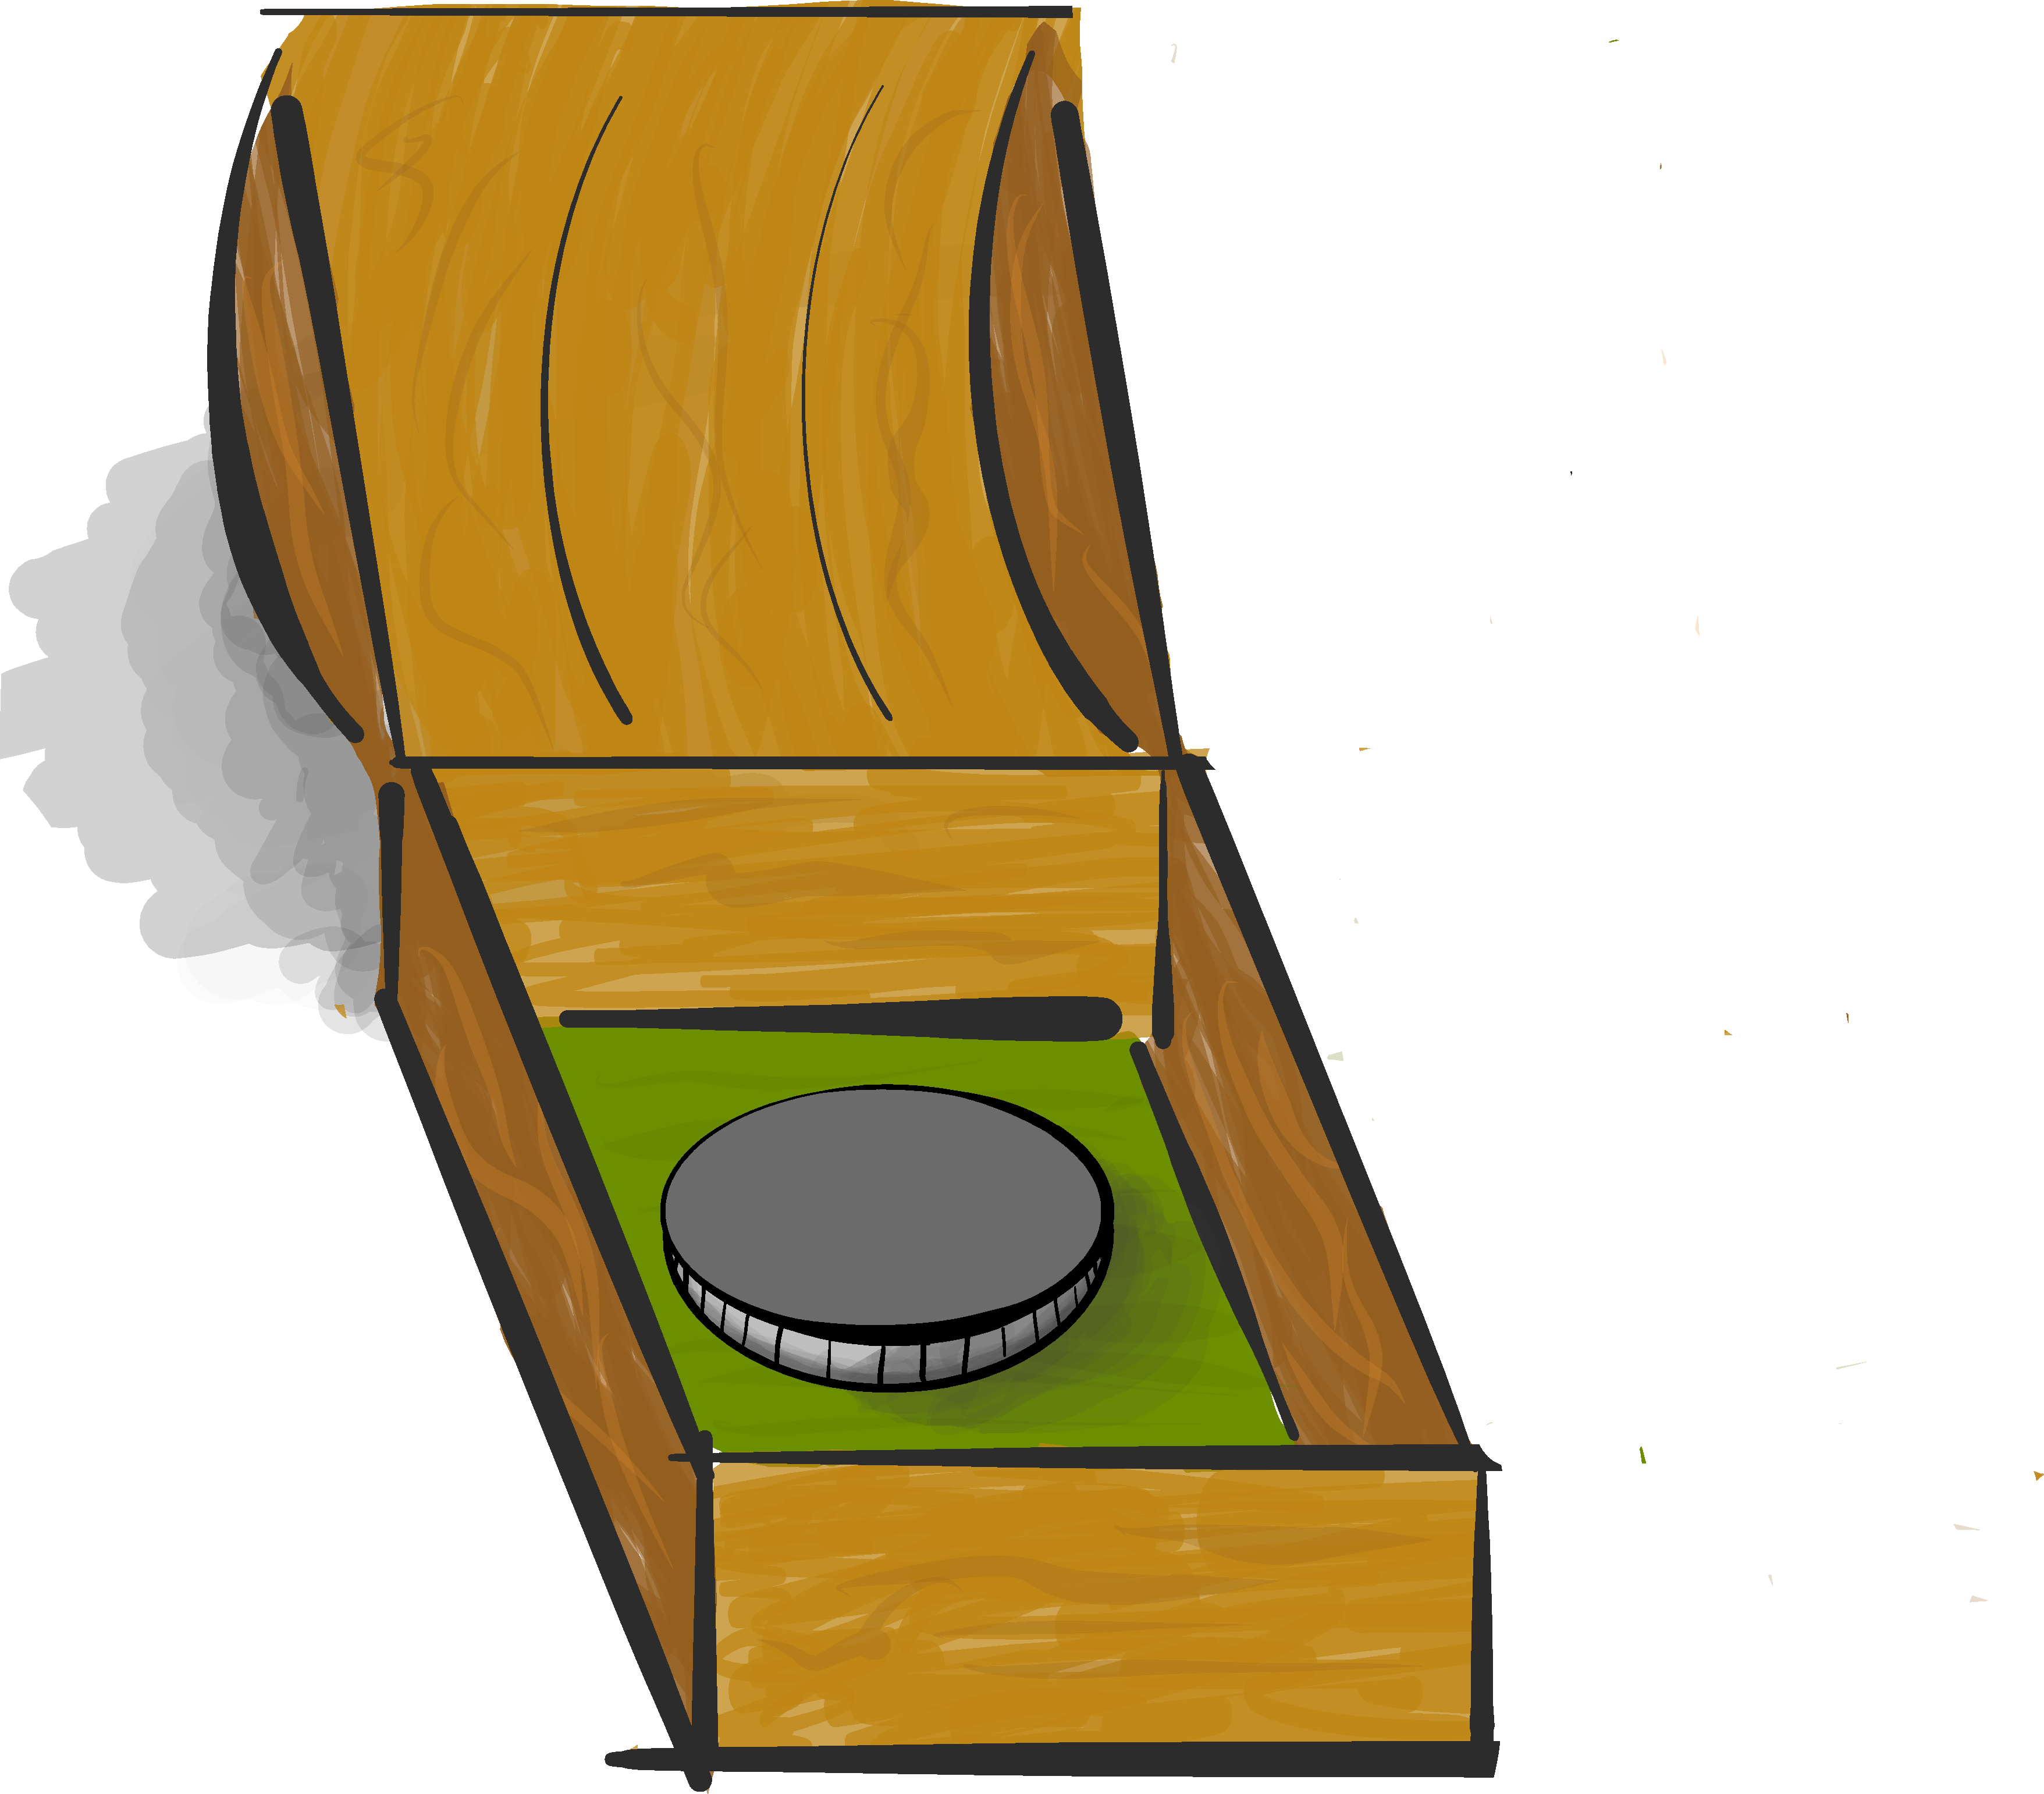
\includegraphics[width=0.3\textwidth]{img/big-box-open-coin}
\end{center}
We are again certain about the state of the coin, so $S = 0$.
This is where \textit{information} comes into play.
\textit{Information} is the difference between two entropies.
We can calculate the information that was gained opening the box by subtracting the ending entropy from the starting entropy,
\begin{align*}
I
&= S_{\text{before}} - S_{\text{after}} \\
&= 1 - 0 \\
&= 1
\end{align*}
We gained one bit of information.
Neat!

We can cement our intuition for what entropy measures by repeating our little thought experiment with a slightly different set up.
Now, instead of a coin we have a die.
The die has ten faces.
Nine of the faces are painted grey.
The last face is painted red.
\begin{center}
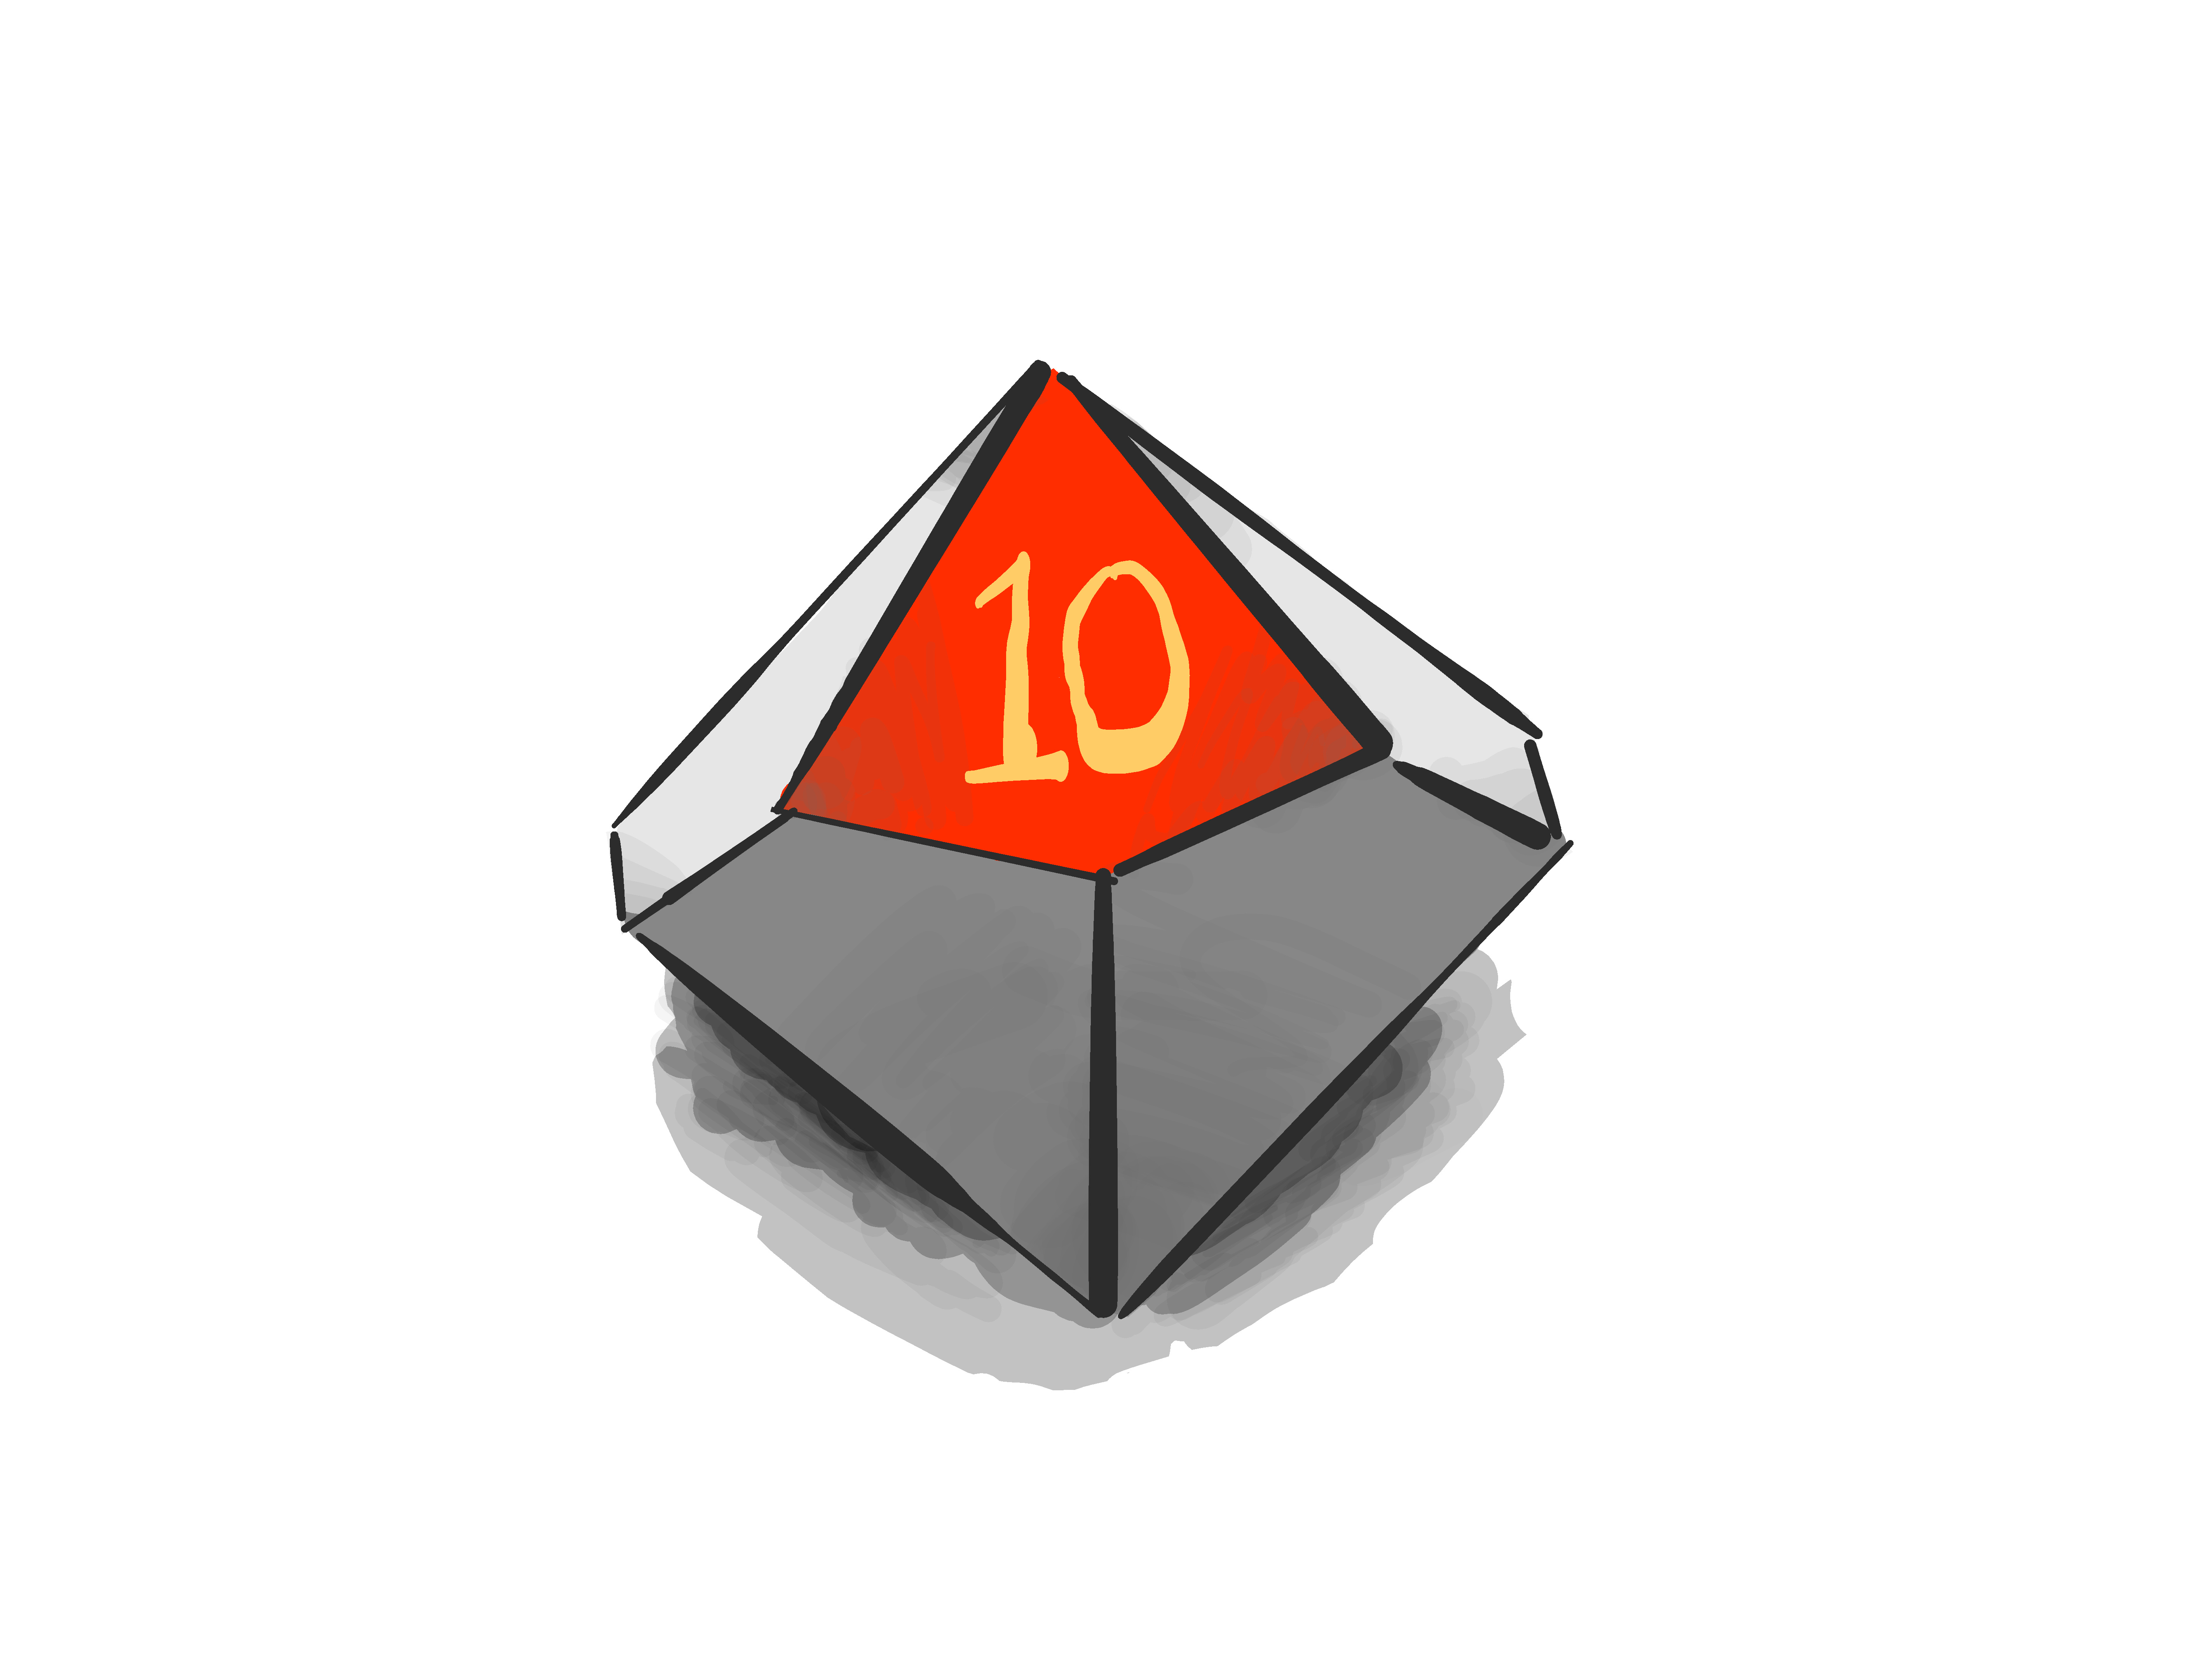
\includegraphics[width=0.3\textwidth]{img/red-die}
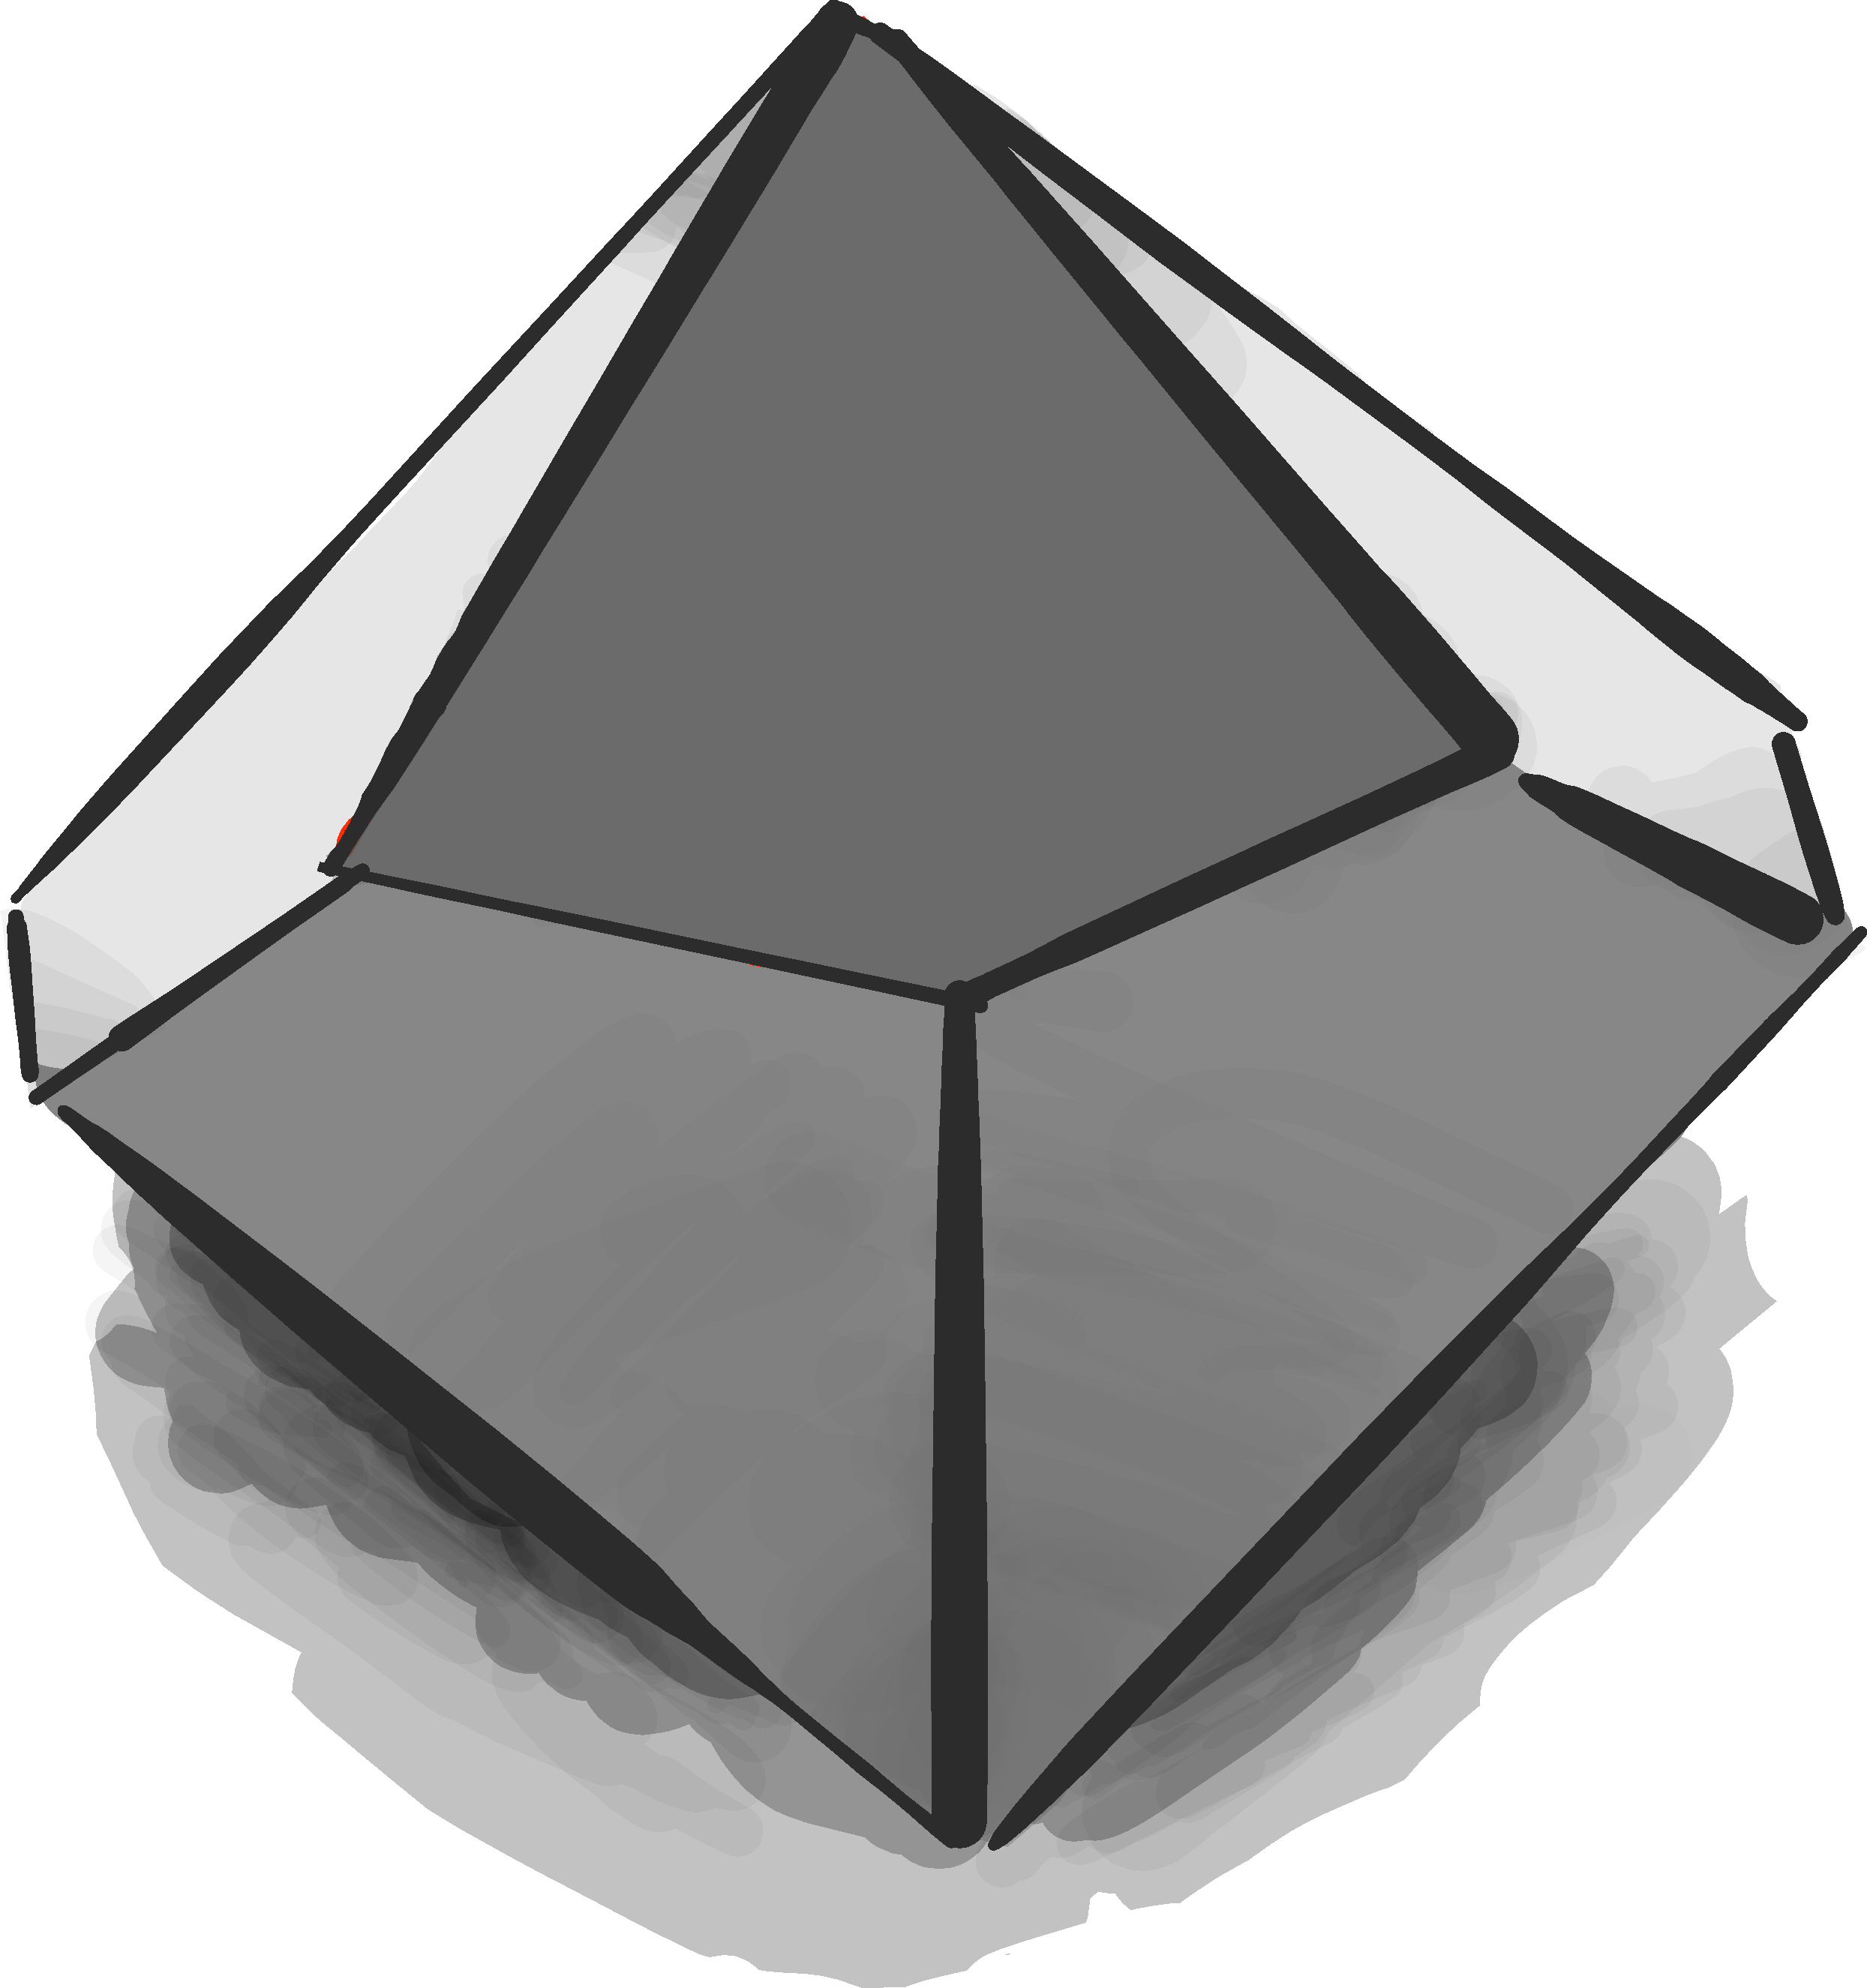
\includegraphics[width=0.3\textwidth]{img/grey-die}
\end{center}
The die is evenly weighted;
if we were to throw it in the air, it would land at equal frequency with any of its ten sides up.
Thus, nine times out of ten it will land with a grey side up and one time out of ten it will land with the red side up.
If we model our die as a random variable $\bm{D}$, we can write this mathematically as $p_{\bm{D} = \text{red}} = 0.1$ and $p_{\bm{D} = \text{grey}} = 0.9$.

Let's put the die in a box, like so.
\begin{center}
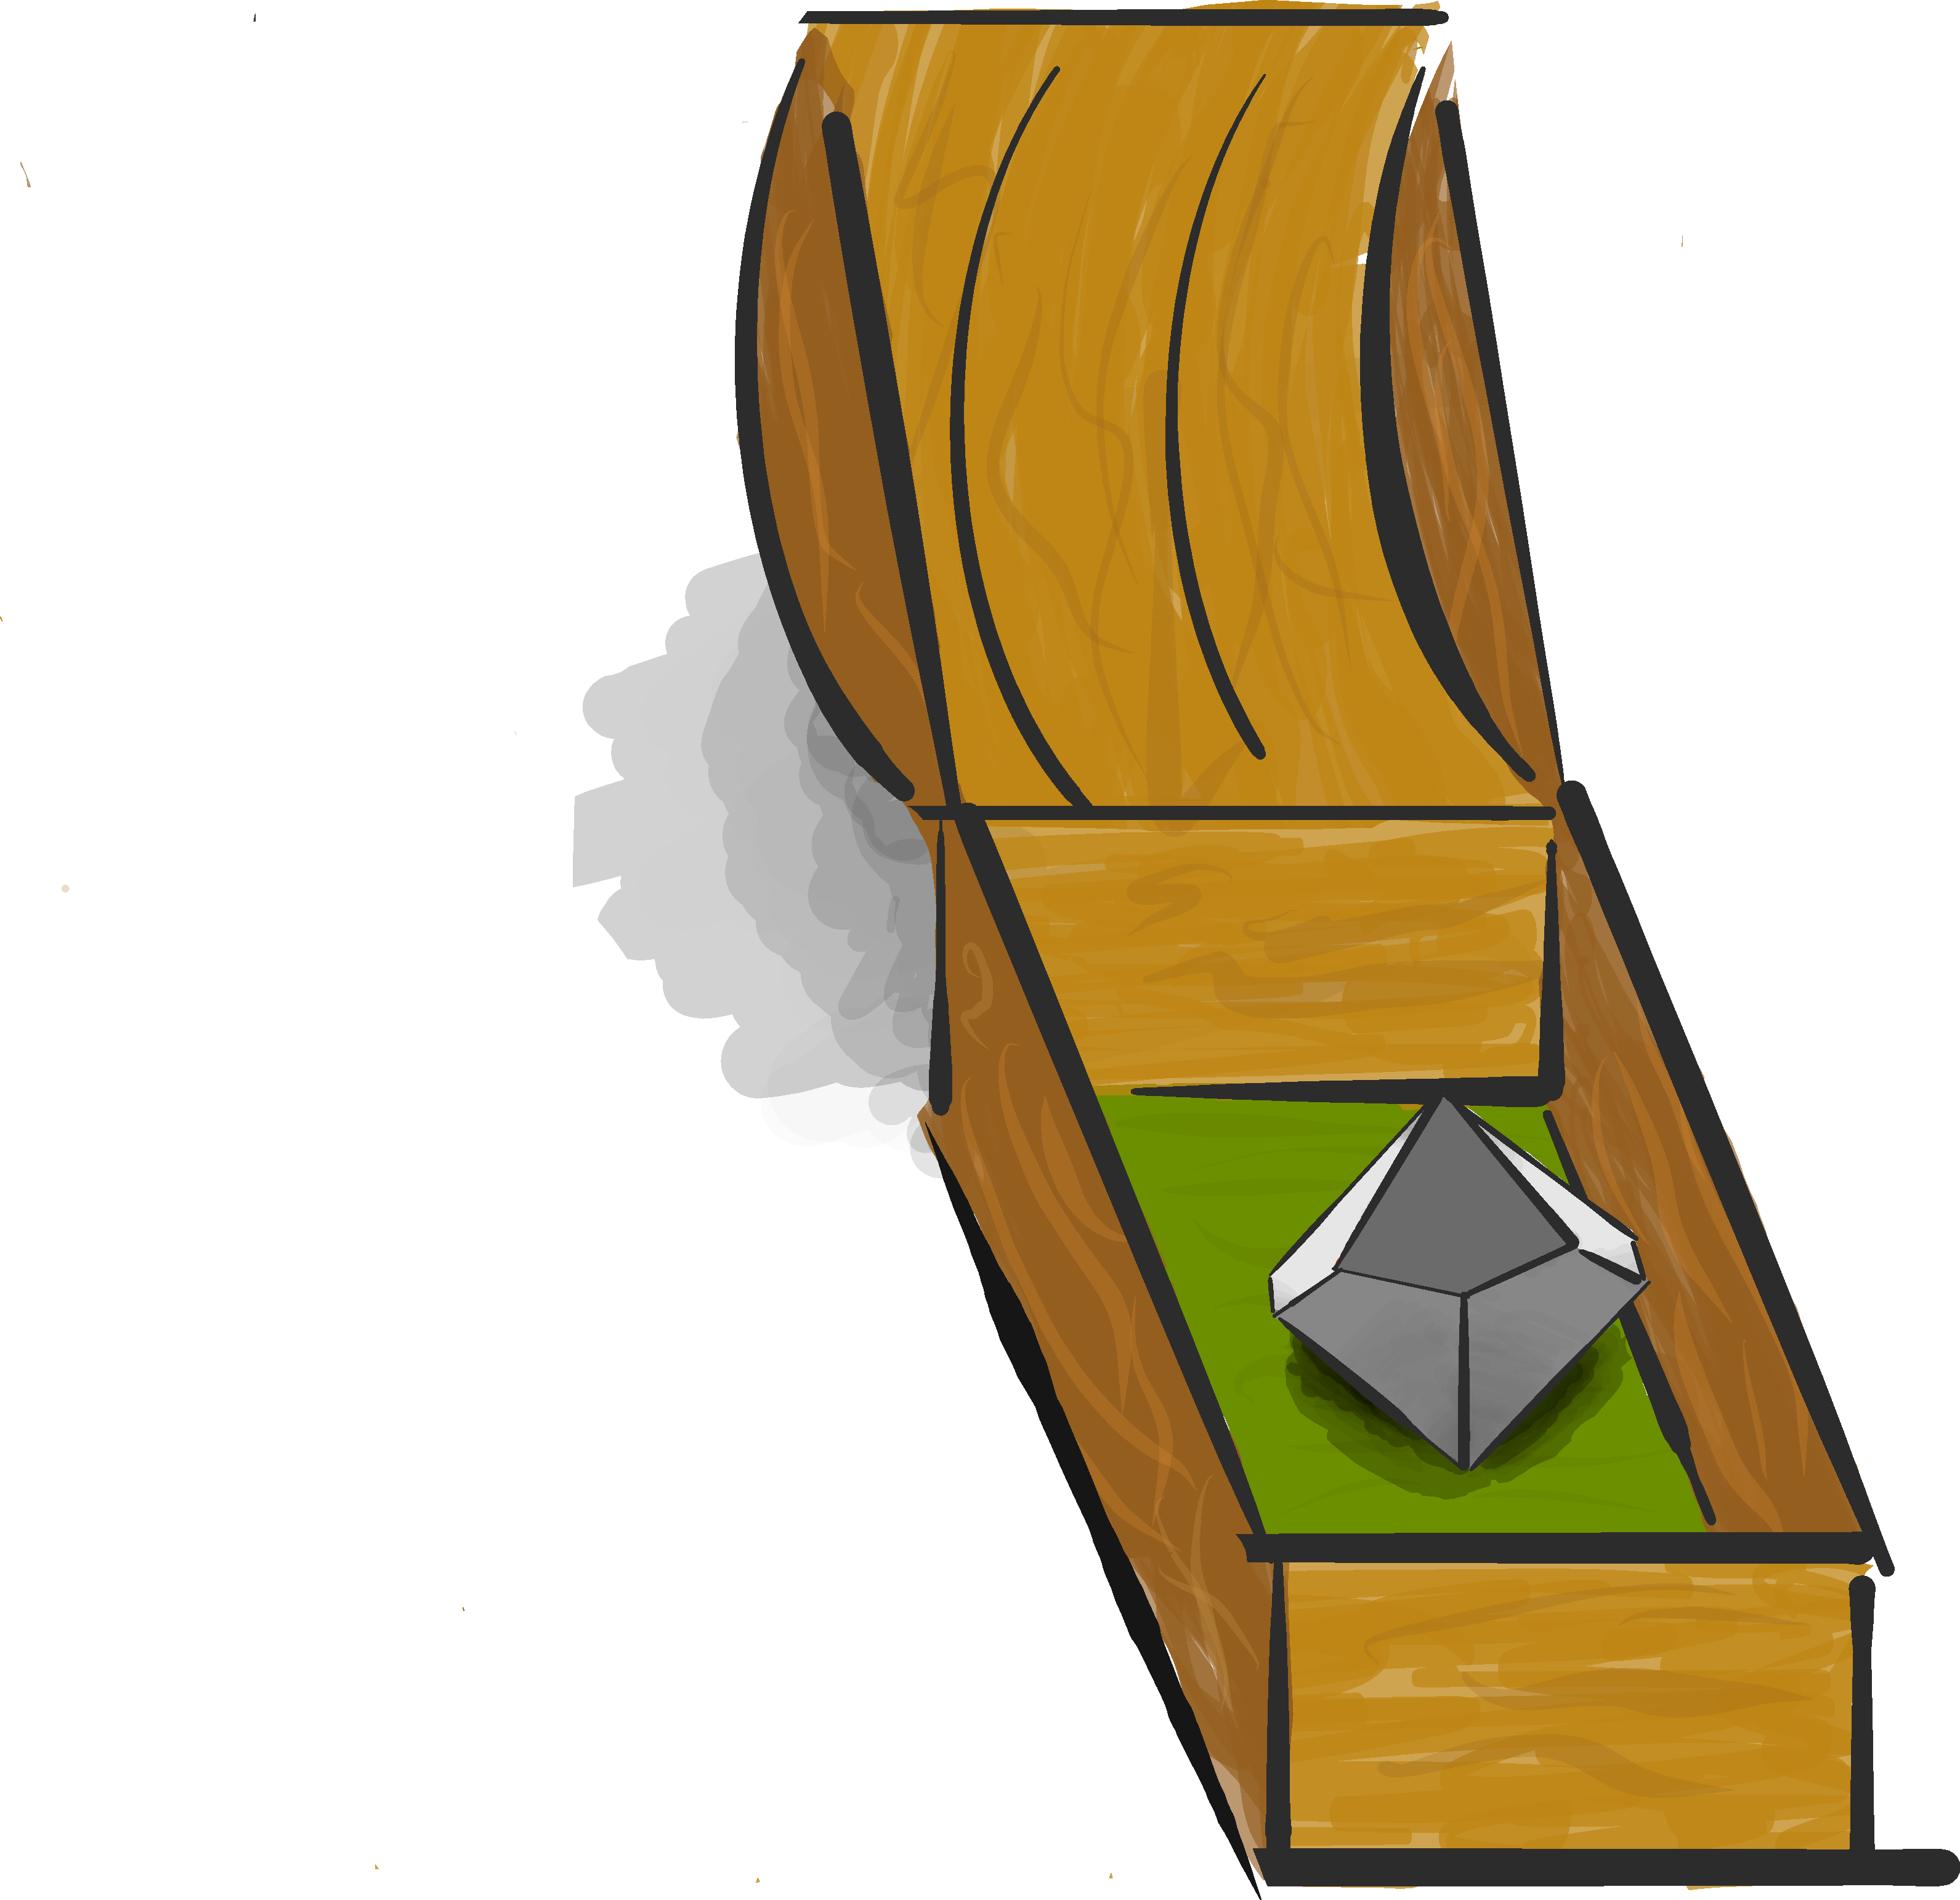
\includegraphics[width=0.3\textwidth]{img/small-box-open-die}
\end{center}
We close the box and give it a shake.
\begin{center}
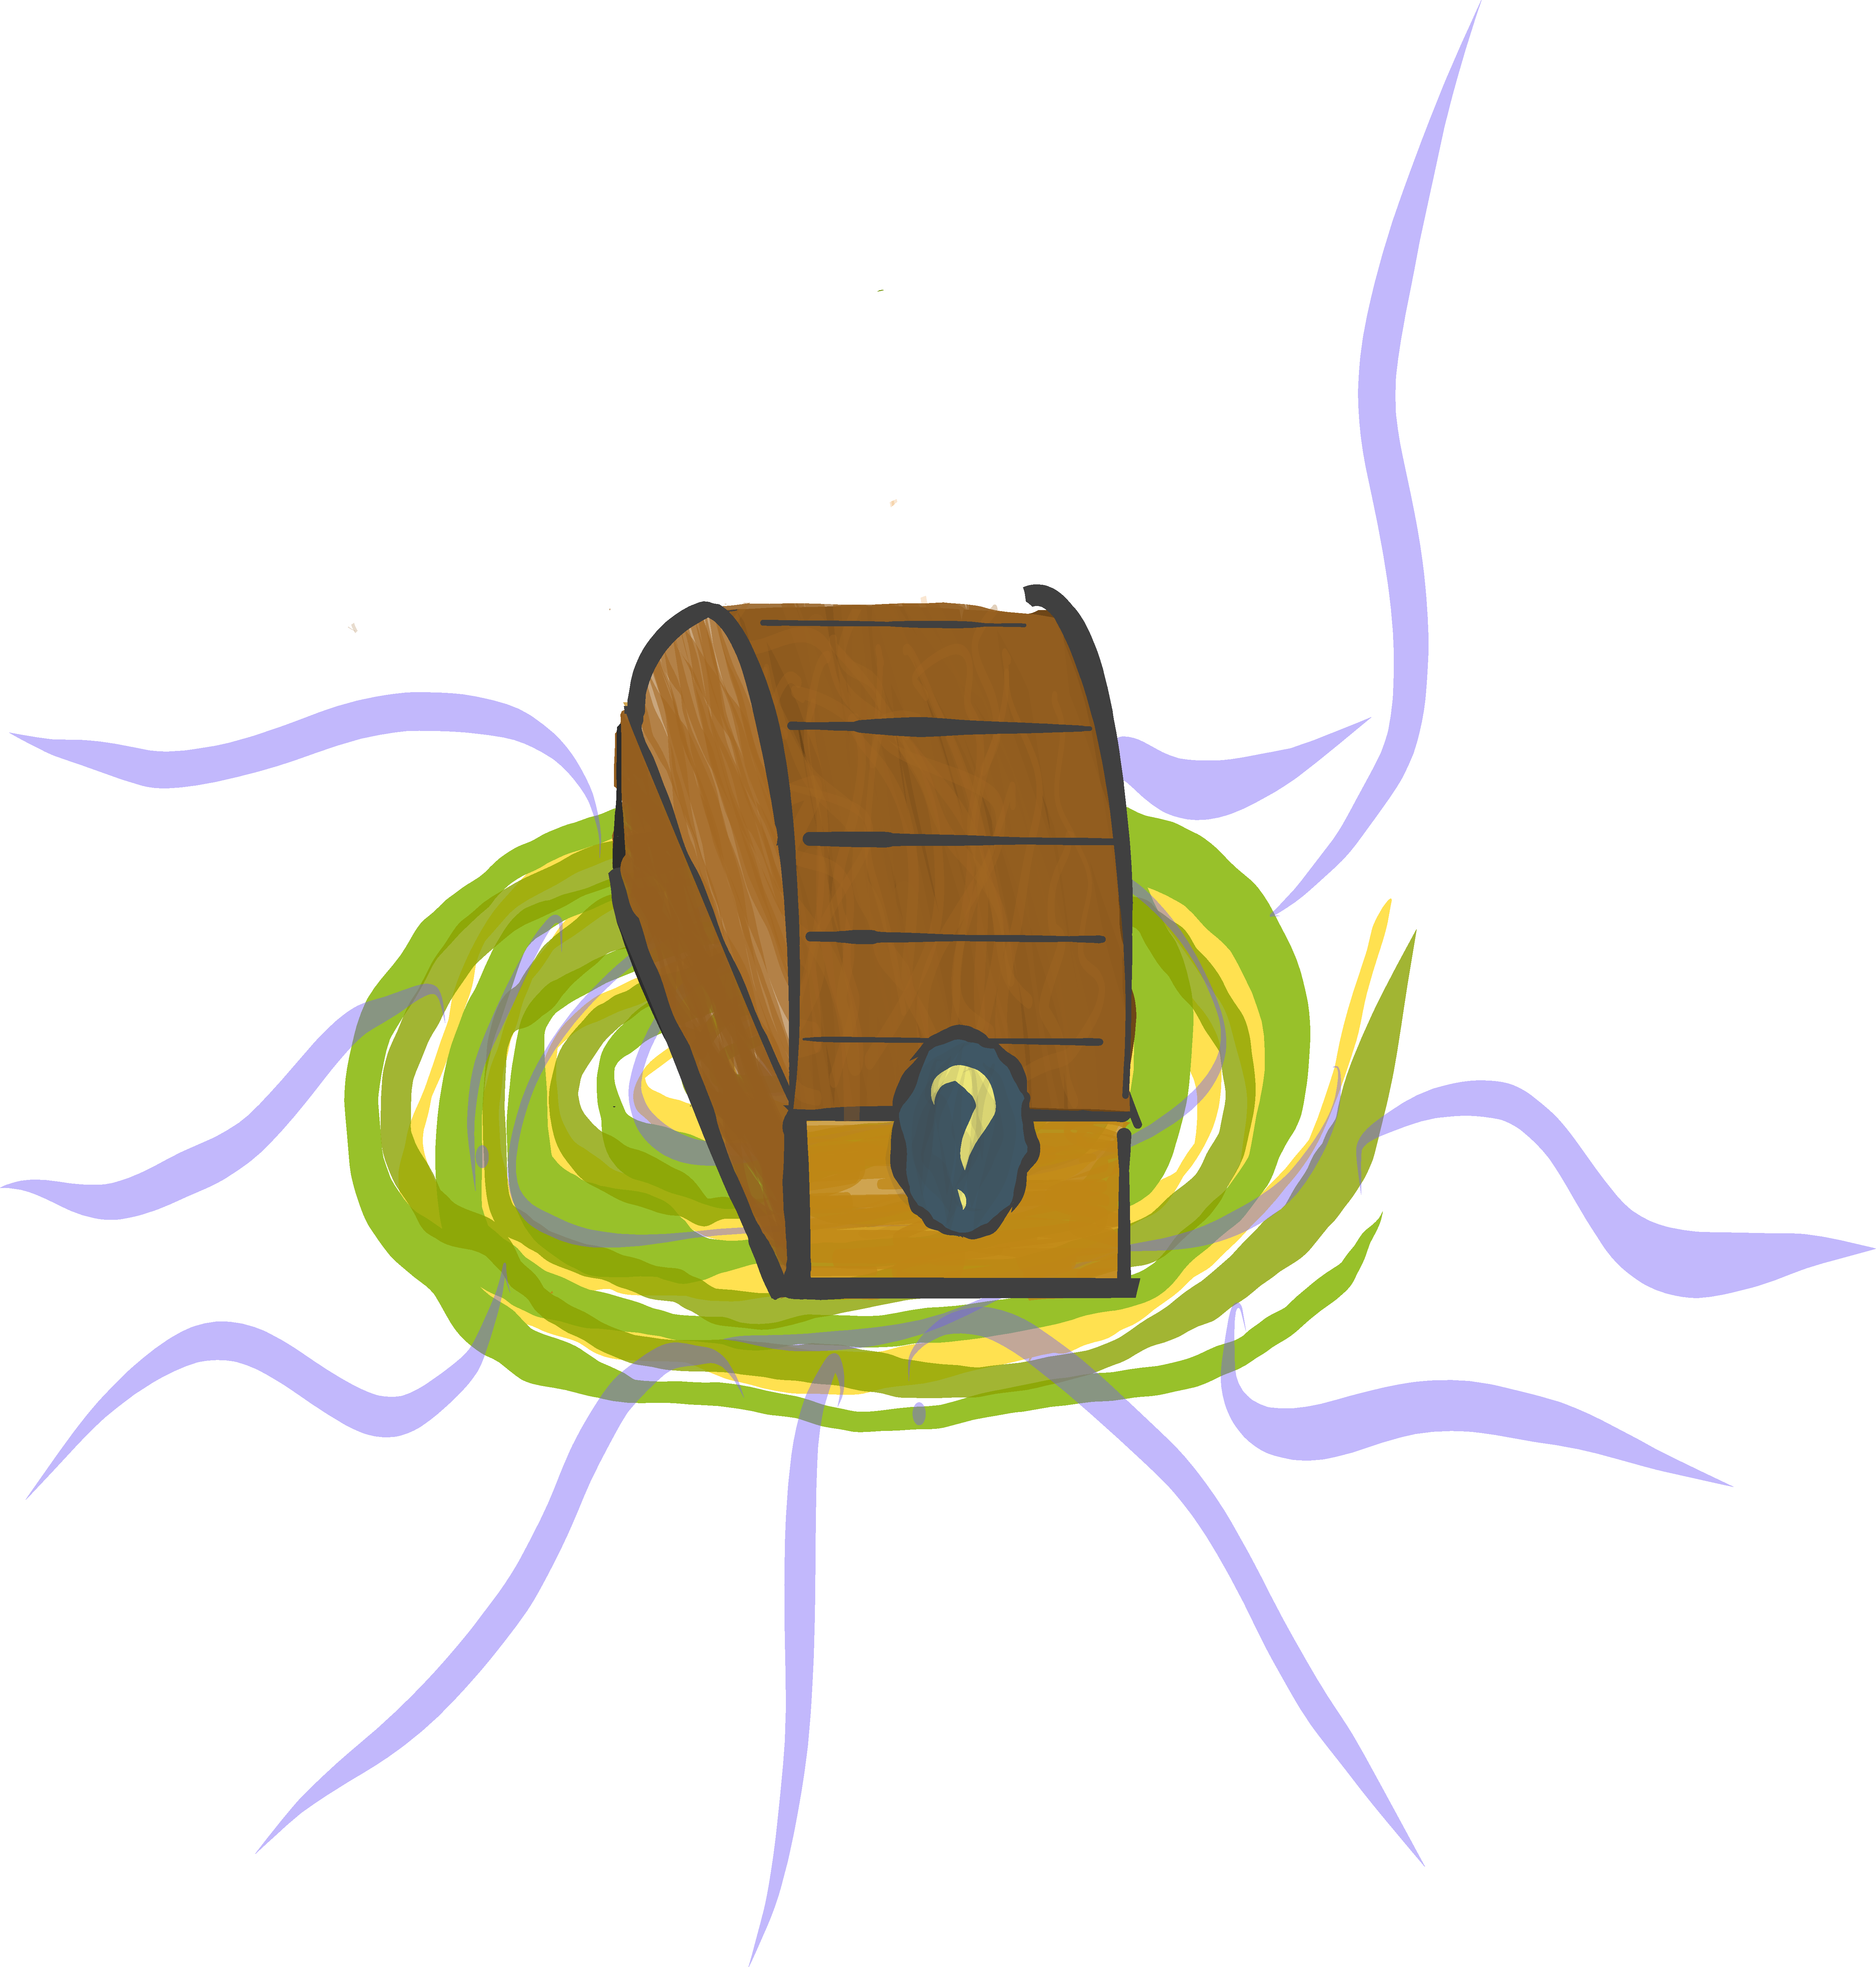
\includegraphics[width=0.5\textwidth]{img/small-box-closed-portal}
\end{center}
We're no longer certain which color is facing up.
As before with the coin, we're faced with uncertainty.
This raises a key question: are we more uncertain about the color facing up of the die than about the color facing up of the coin?

Let's think through it.
Observing both the coin and the die, we recognize two outcomes: red side up or grey side up.
The difference is that for the coin, these outcomes have equal probability.
For the die, it is more likely that we will observe the grey outcome.
Thus, we can make a better guess as to what outcome we will observe on the grey die than we can for the coin.
If we always guess grey on the die, we will be correct much more often than if we always guessed grey on the coin.
So, we would expect that there is more uncertainty associated with the coin than with the die.

We can use Shannon's equation (\ref{eqn:shannon}) to formally determine whether the flipped coin or rolled die has more entropy.
We will calculate the entropy of the die in the box and then compare it with the entropy of the coin in the box.
Plugging and chugging with Equation \ref{eqn:shannon}, we calculate
\begin{align*}
S_{\text{die}}
&= H(\bm{D}) \\
&= -0.1 \log(0.1) + -0.9 \log(0.9) \\
&\approx 0.469.
\end{align*}
The die in the box has approximately 0.469 bits of entropy.
It follows that when we open the box with the die in it (and entropy returns to zero), we gain 0.469 bits of information.


\section{Independent Random Variables}

But, wait!
There's more fun to be had with the coin and the die.
Let's take our two boxes and screw them together.
\begin{center}
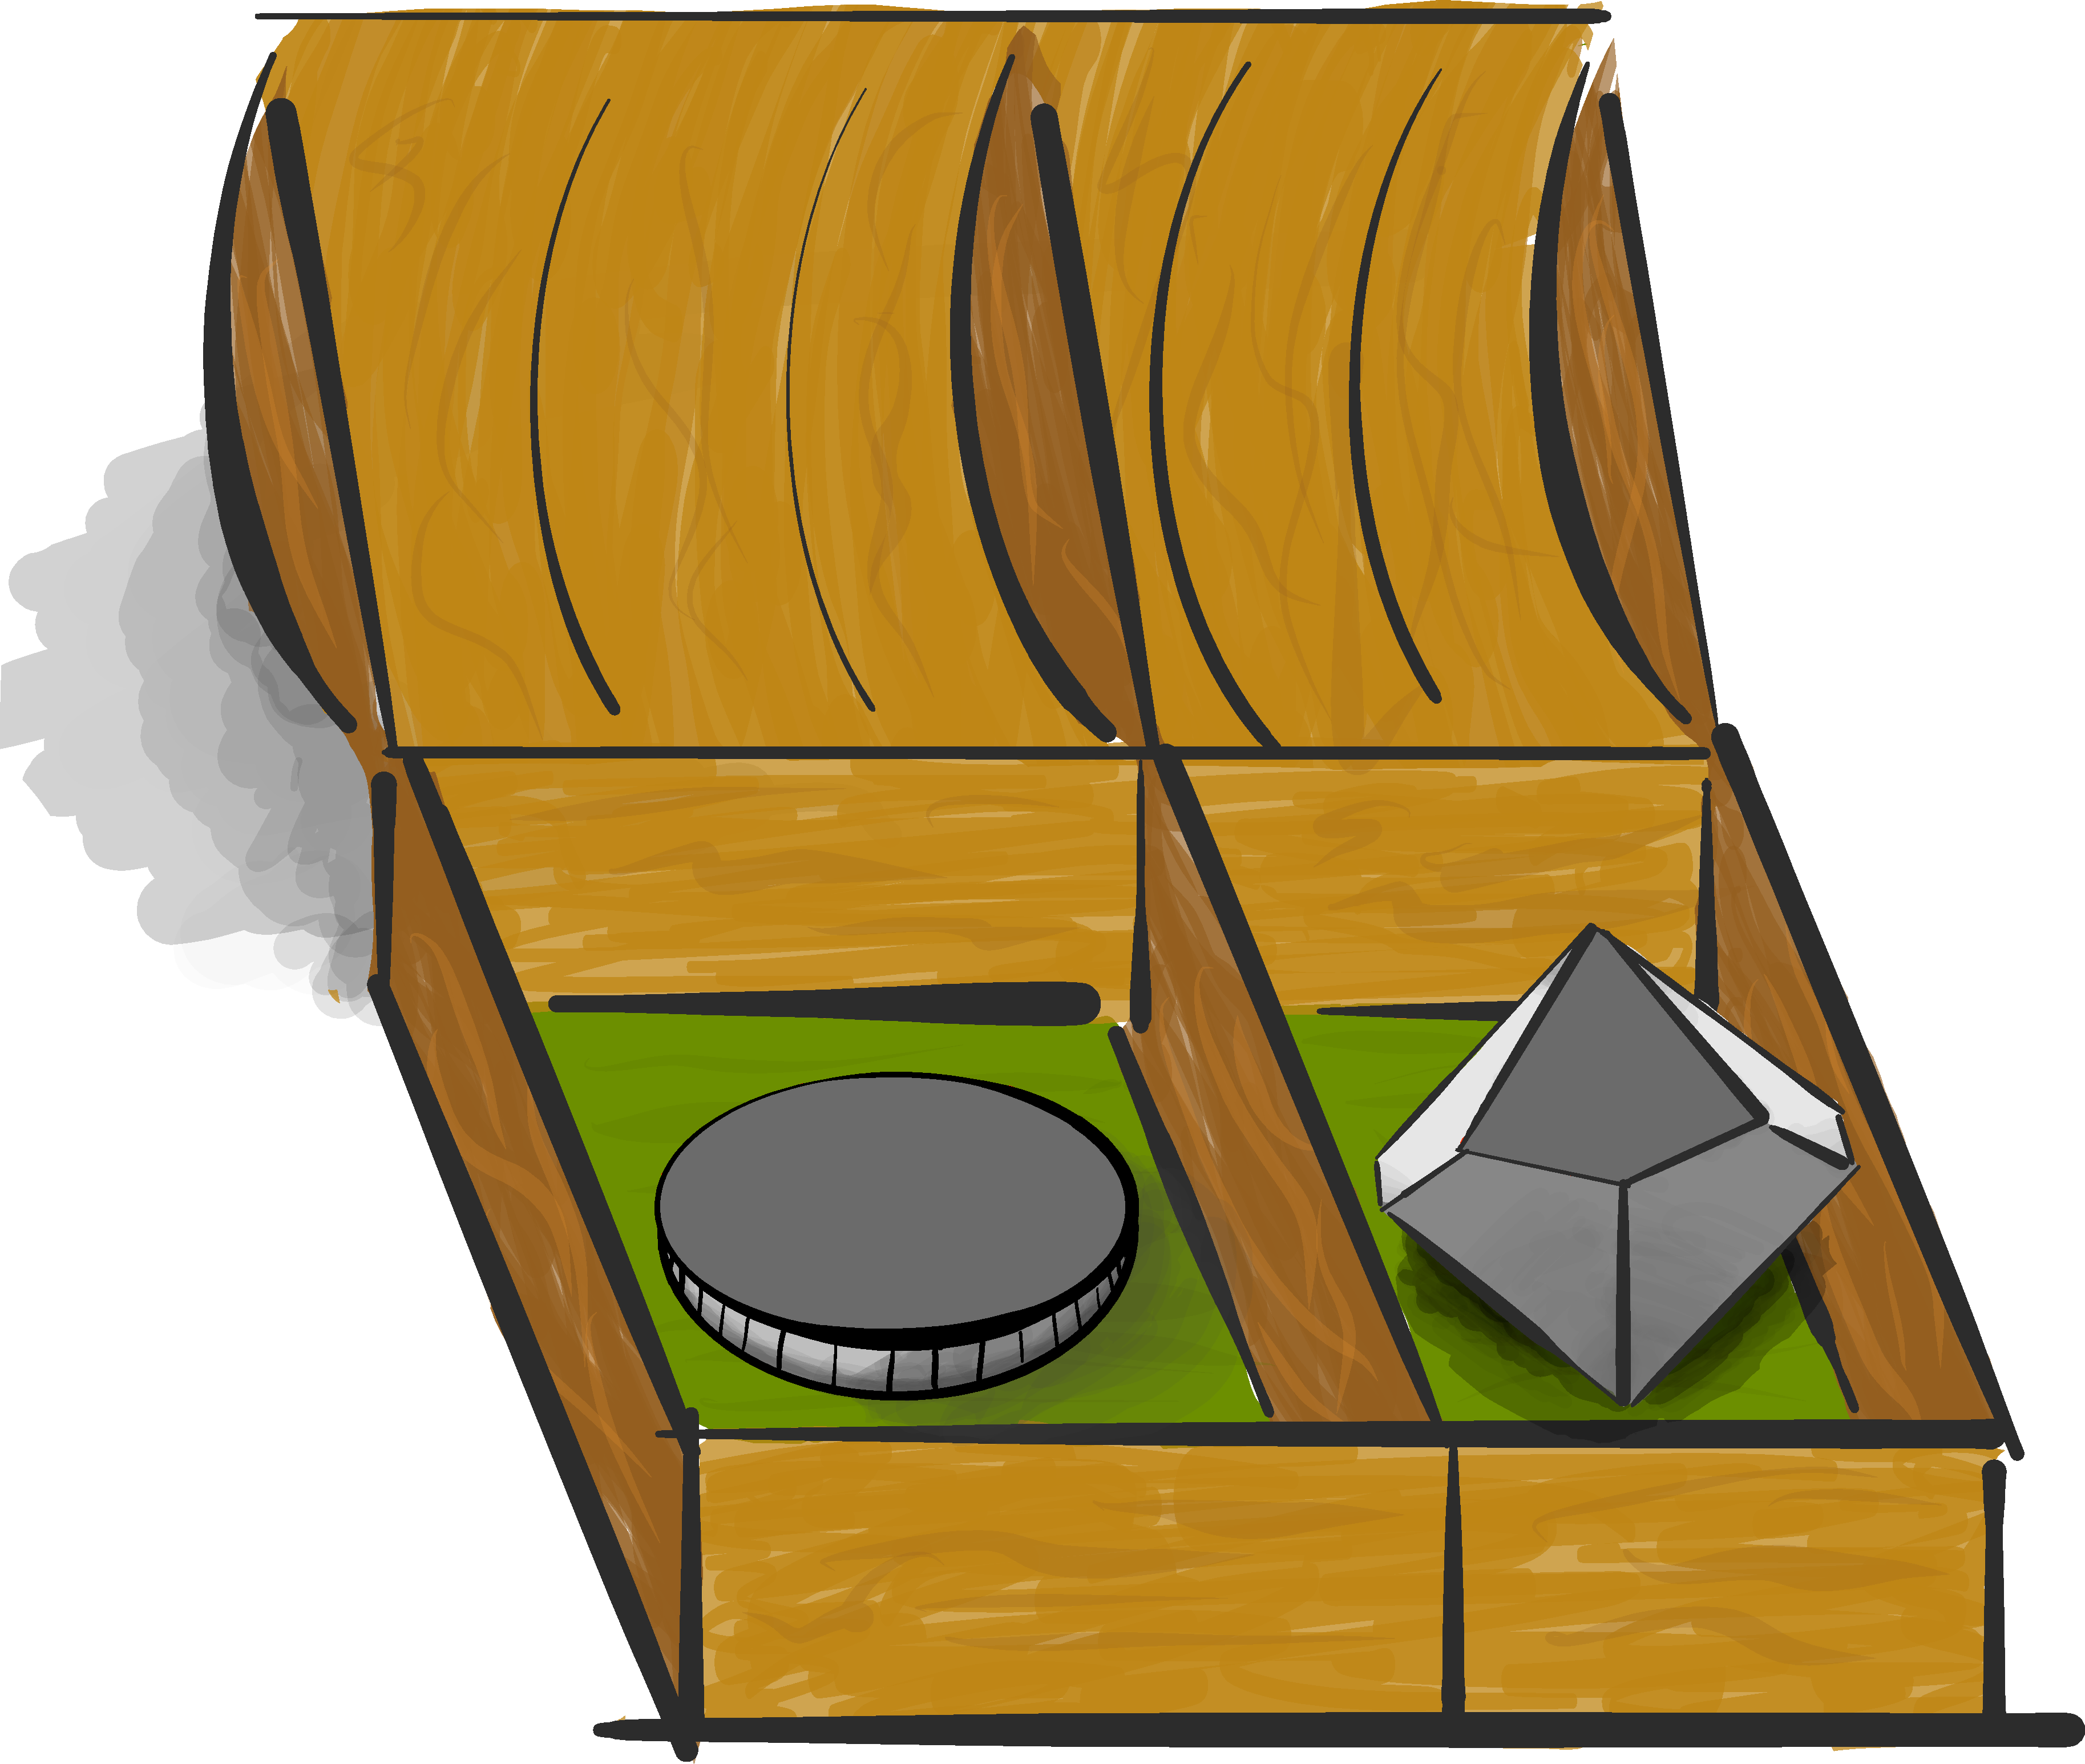
\includegraphics[width=0.4\textwidth]{img/box-both-open-coin-die}
\end{center}
As before, let's close both lids and give the big box a shake.
\begin{center}
\includegraphics[width=\textwidth]{img/both-box-closed-portal}
\end{center}
We will model the big box as a single random variable $\bm{A}$.
Now, there are four possible states that our big box could be in.
Both the coin and the die could be red side up or grey side up.
The possible states of the big box are summarized below.
\begin{center}
 \begin{tabular}{c c || c | c }
 \multicolumn{2}{c}{\multirow{2}{*}{$\bm{A}$}} & \multicolumn{2}{c}{$\bm{C}$} \\
\multicolumn{2}{c}{} & red & grey \\ [0.5ex]
 \hline\hline
\multirow{14}{*}{$\bm{D}$} & red
& \makecell{
  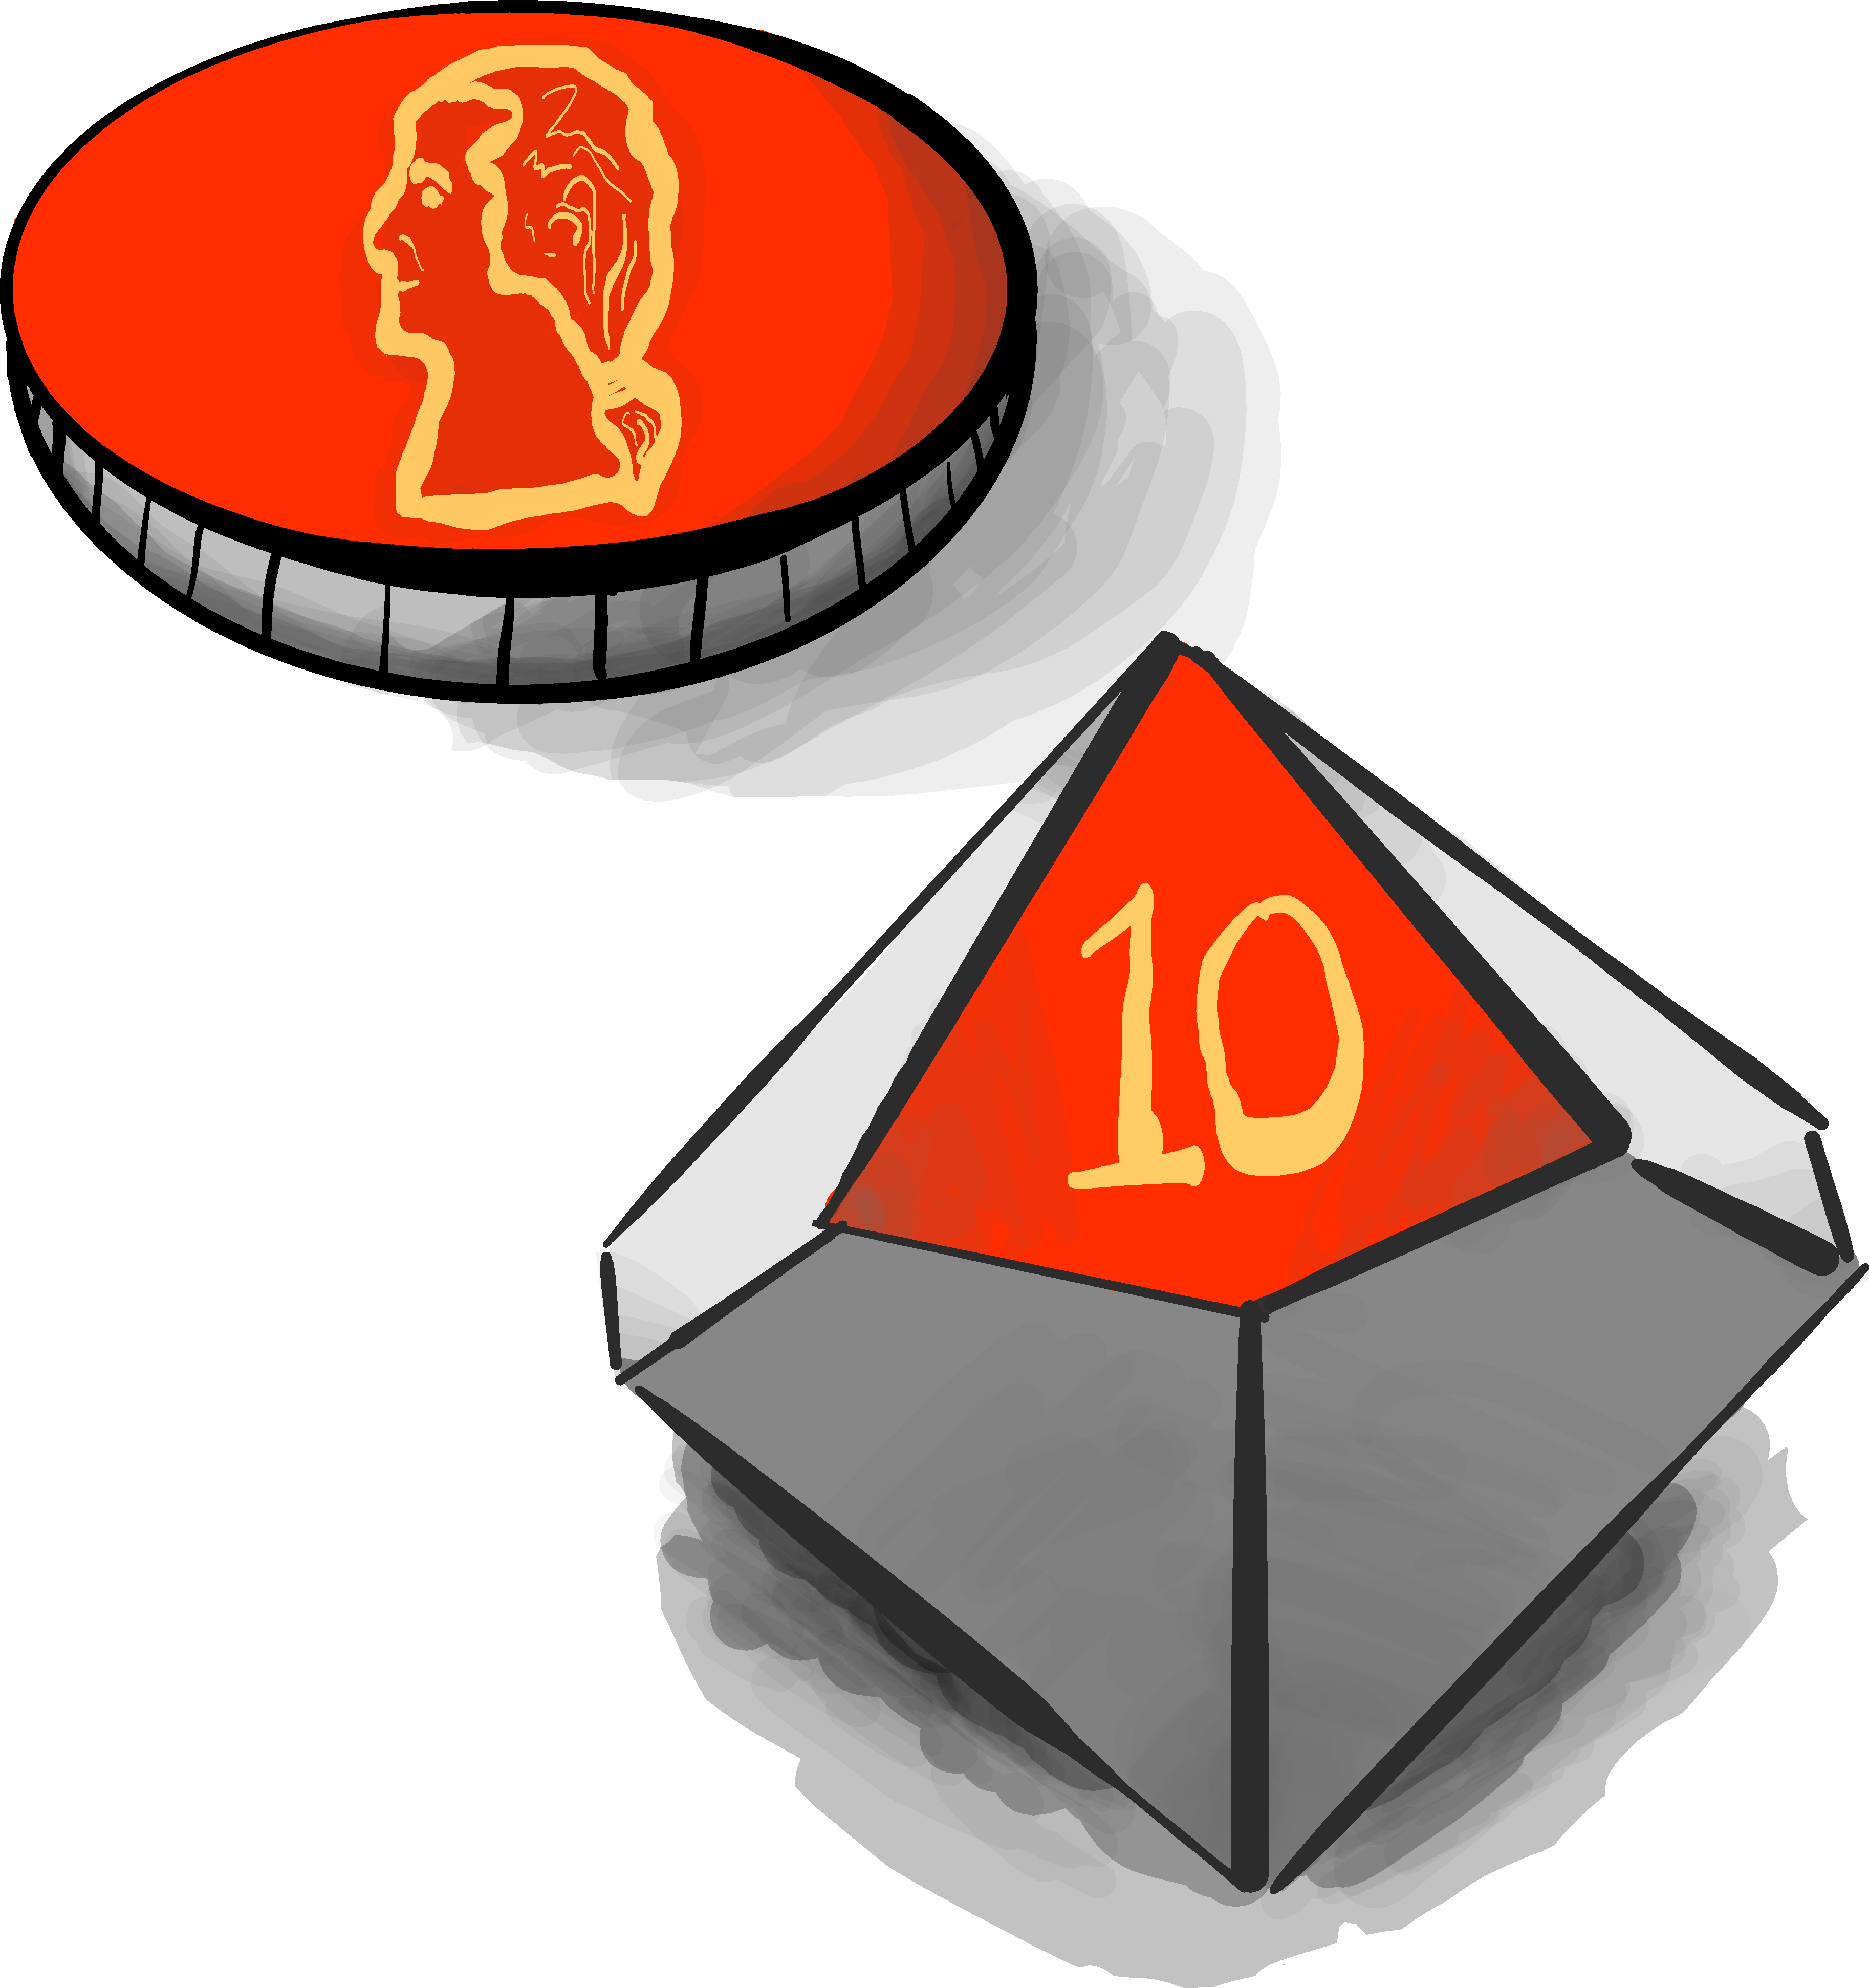
\includegraphics[trim= 0 0 0 -20ex, clip, width=0.3\textwidth]{img/red-coin-red-die} \\
  $\bm{A} = \text{``red coin, red die''}$
  }
 & \makecell{
  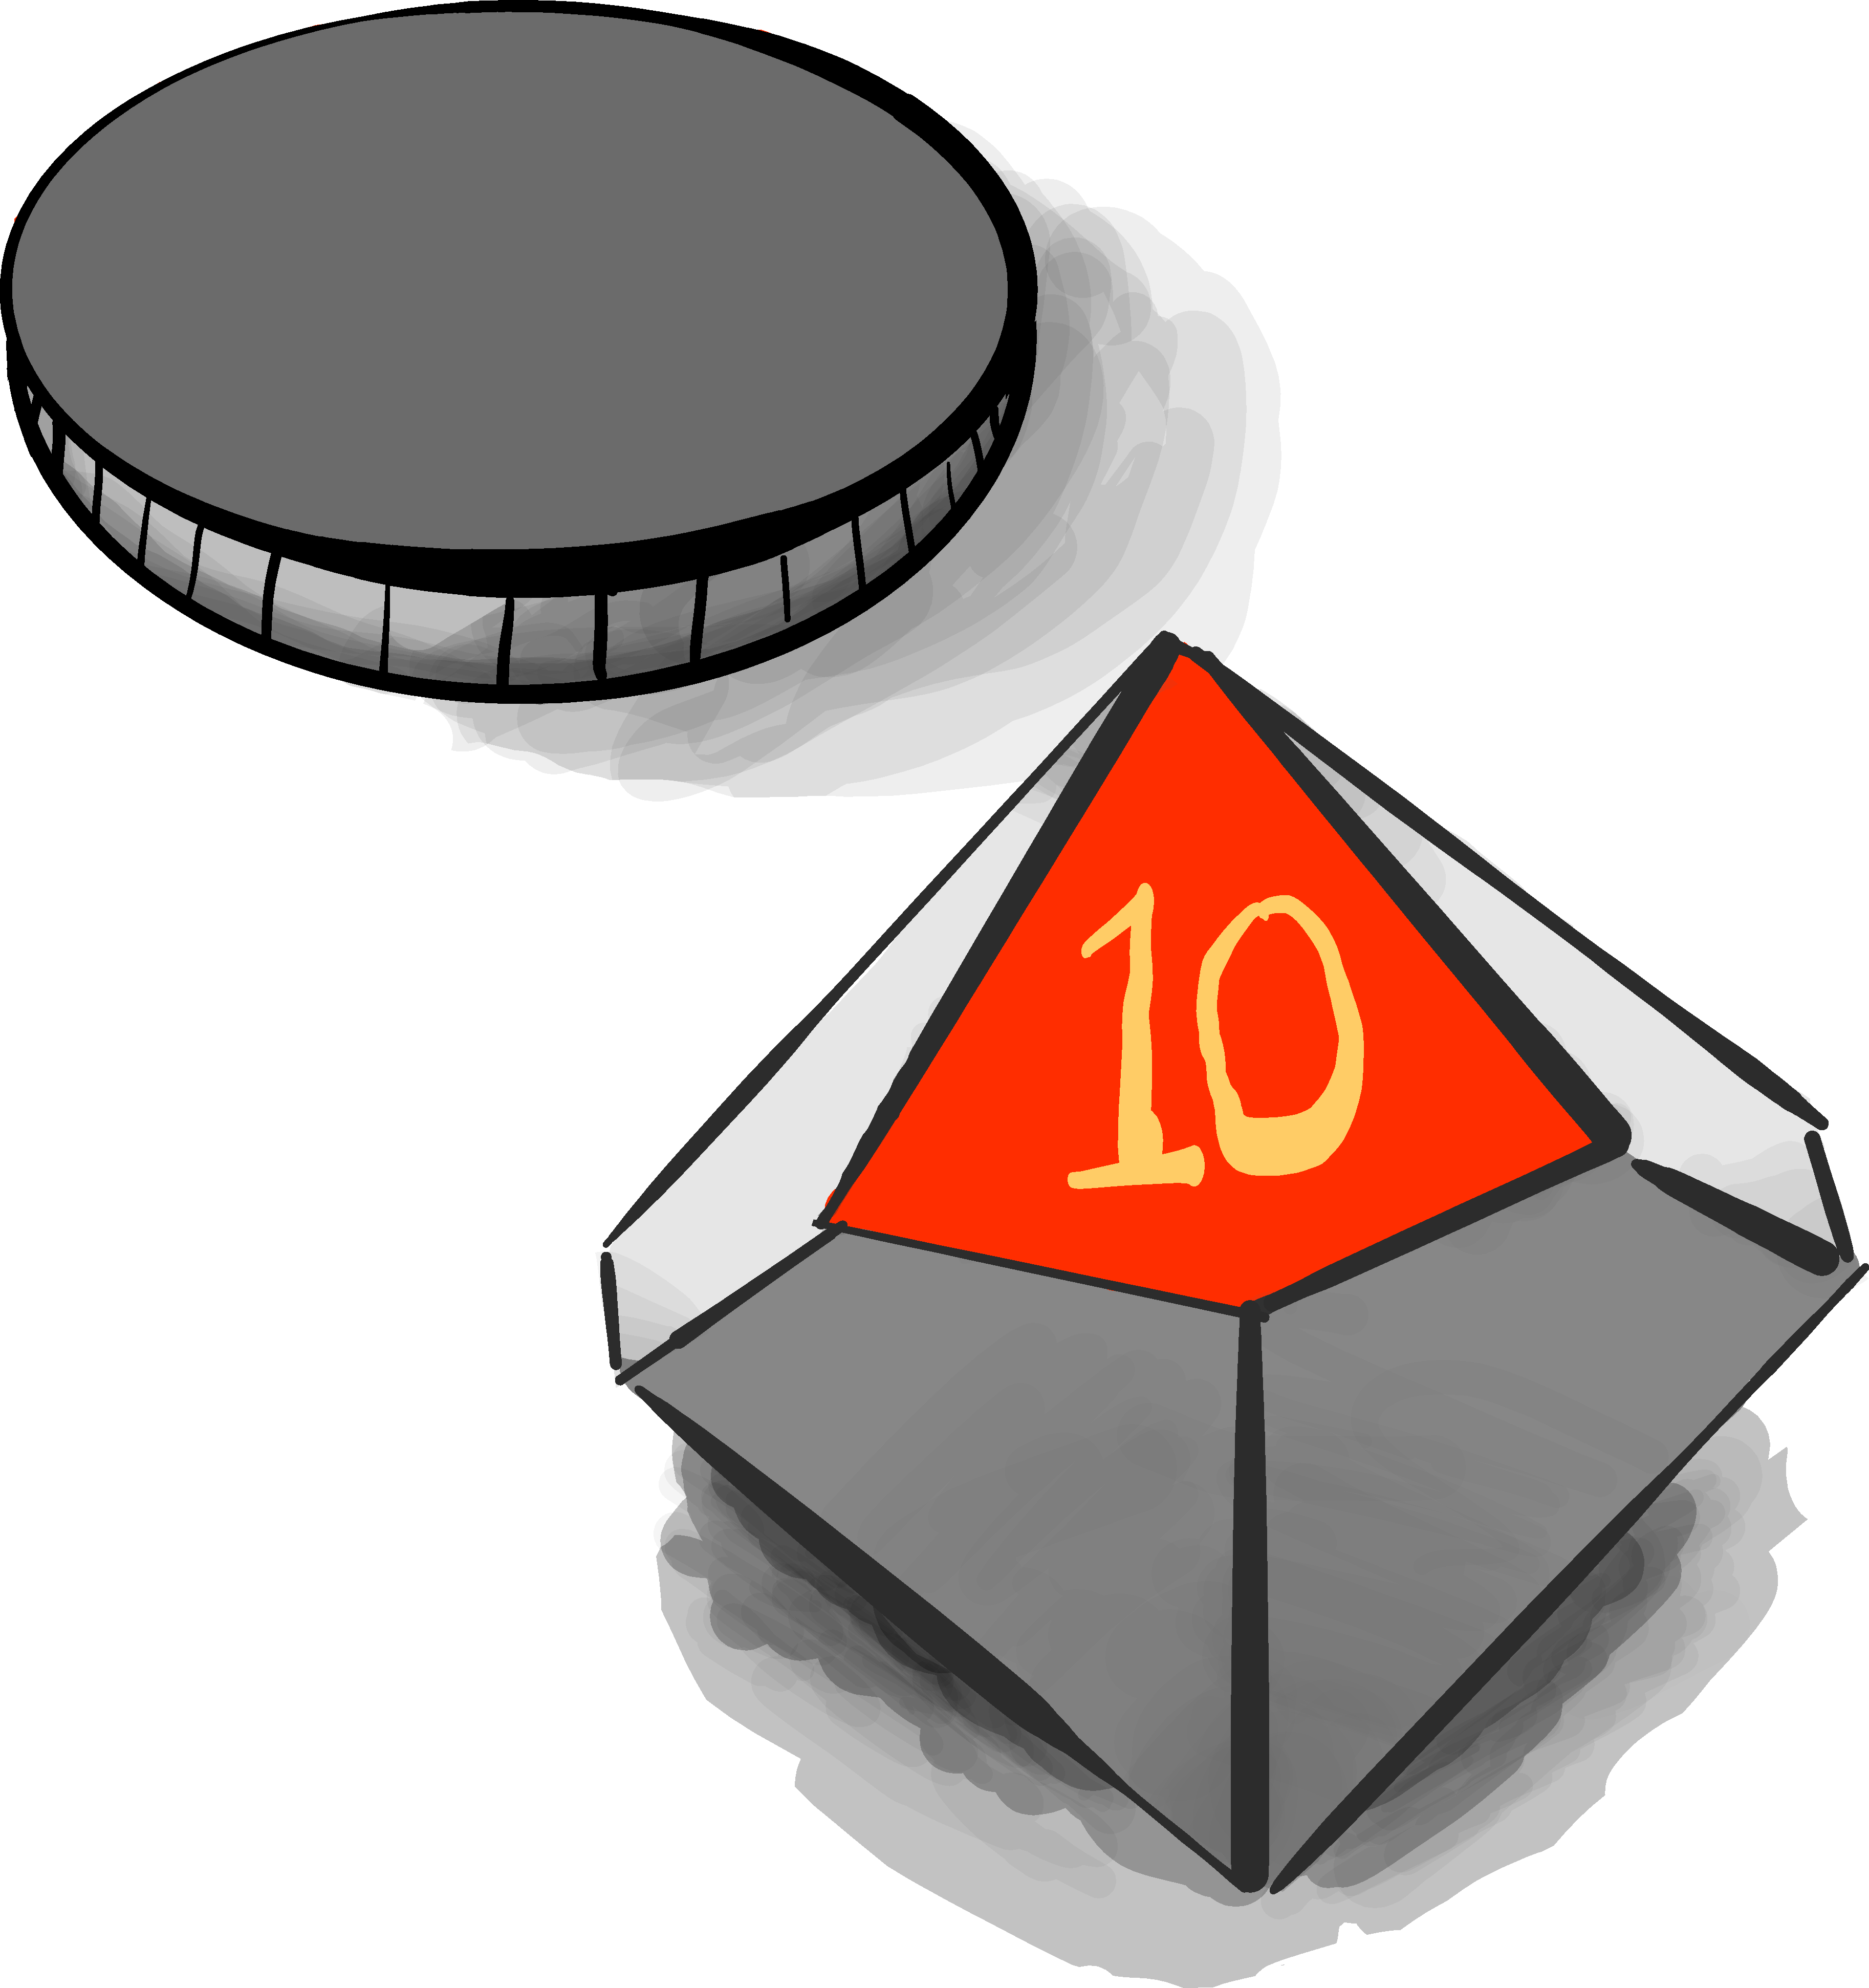
\includegraphics[trim= 0 0 0 -20ex, clip, width=0.3\textwidth]{img/grey-coin-red-die} \\
  $\bm{A} = \text{``grey coin, red die''}$
  }
  \\
 \cline{2-4}
 & grey
 & \makecell{
 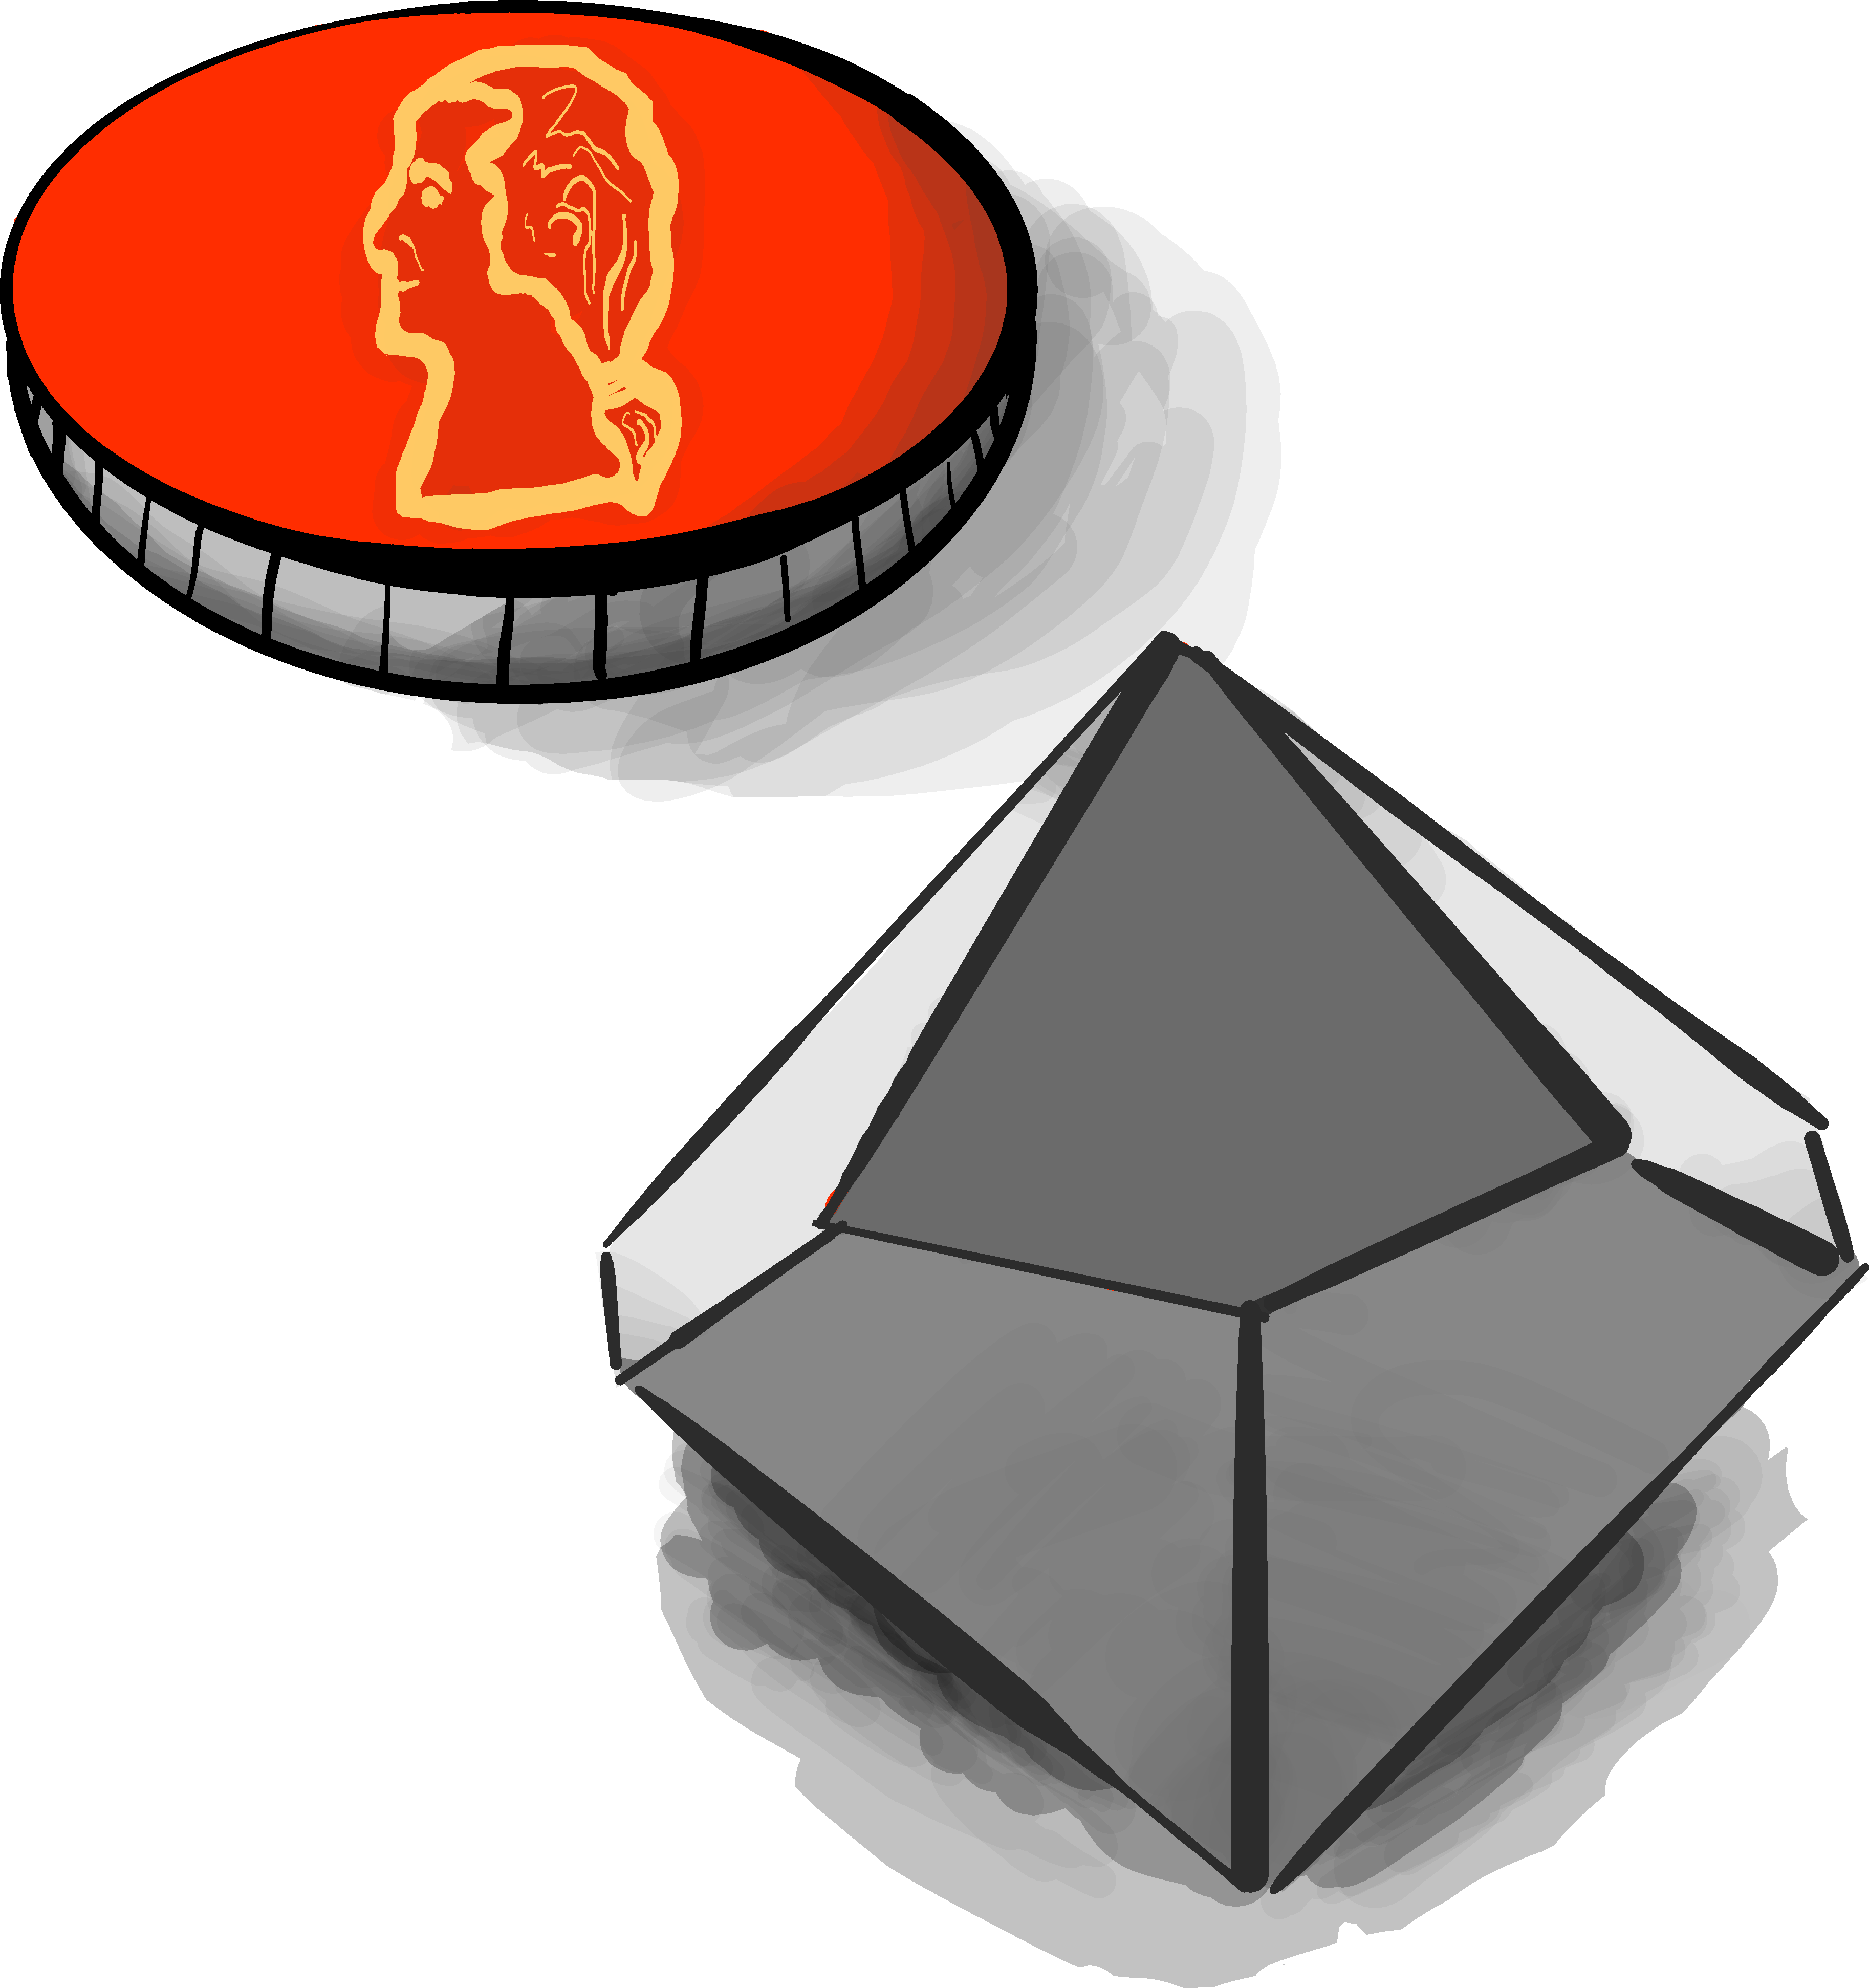
\includegraphics[trim= 0 0 0 -20ex, clip, width=0.3\textwidth]{img/red-coin-grey-die} \\
  $\bm{A} = \text{``red coin, grey die''}$}
 & \makecell{
 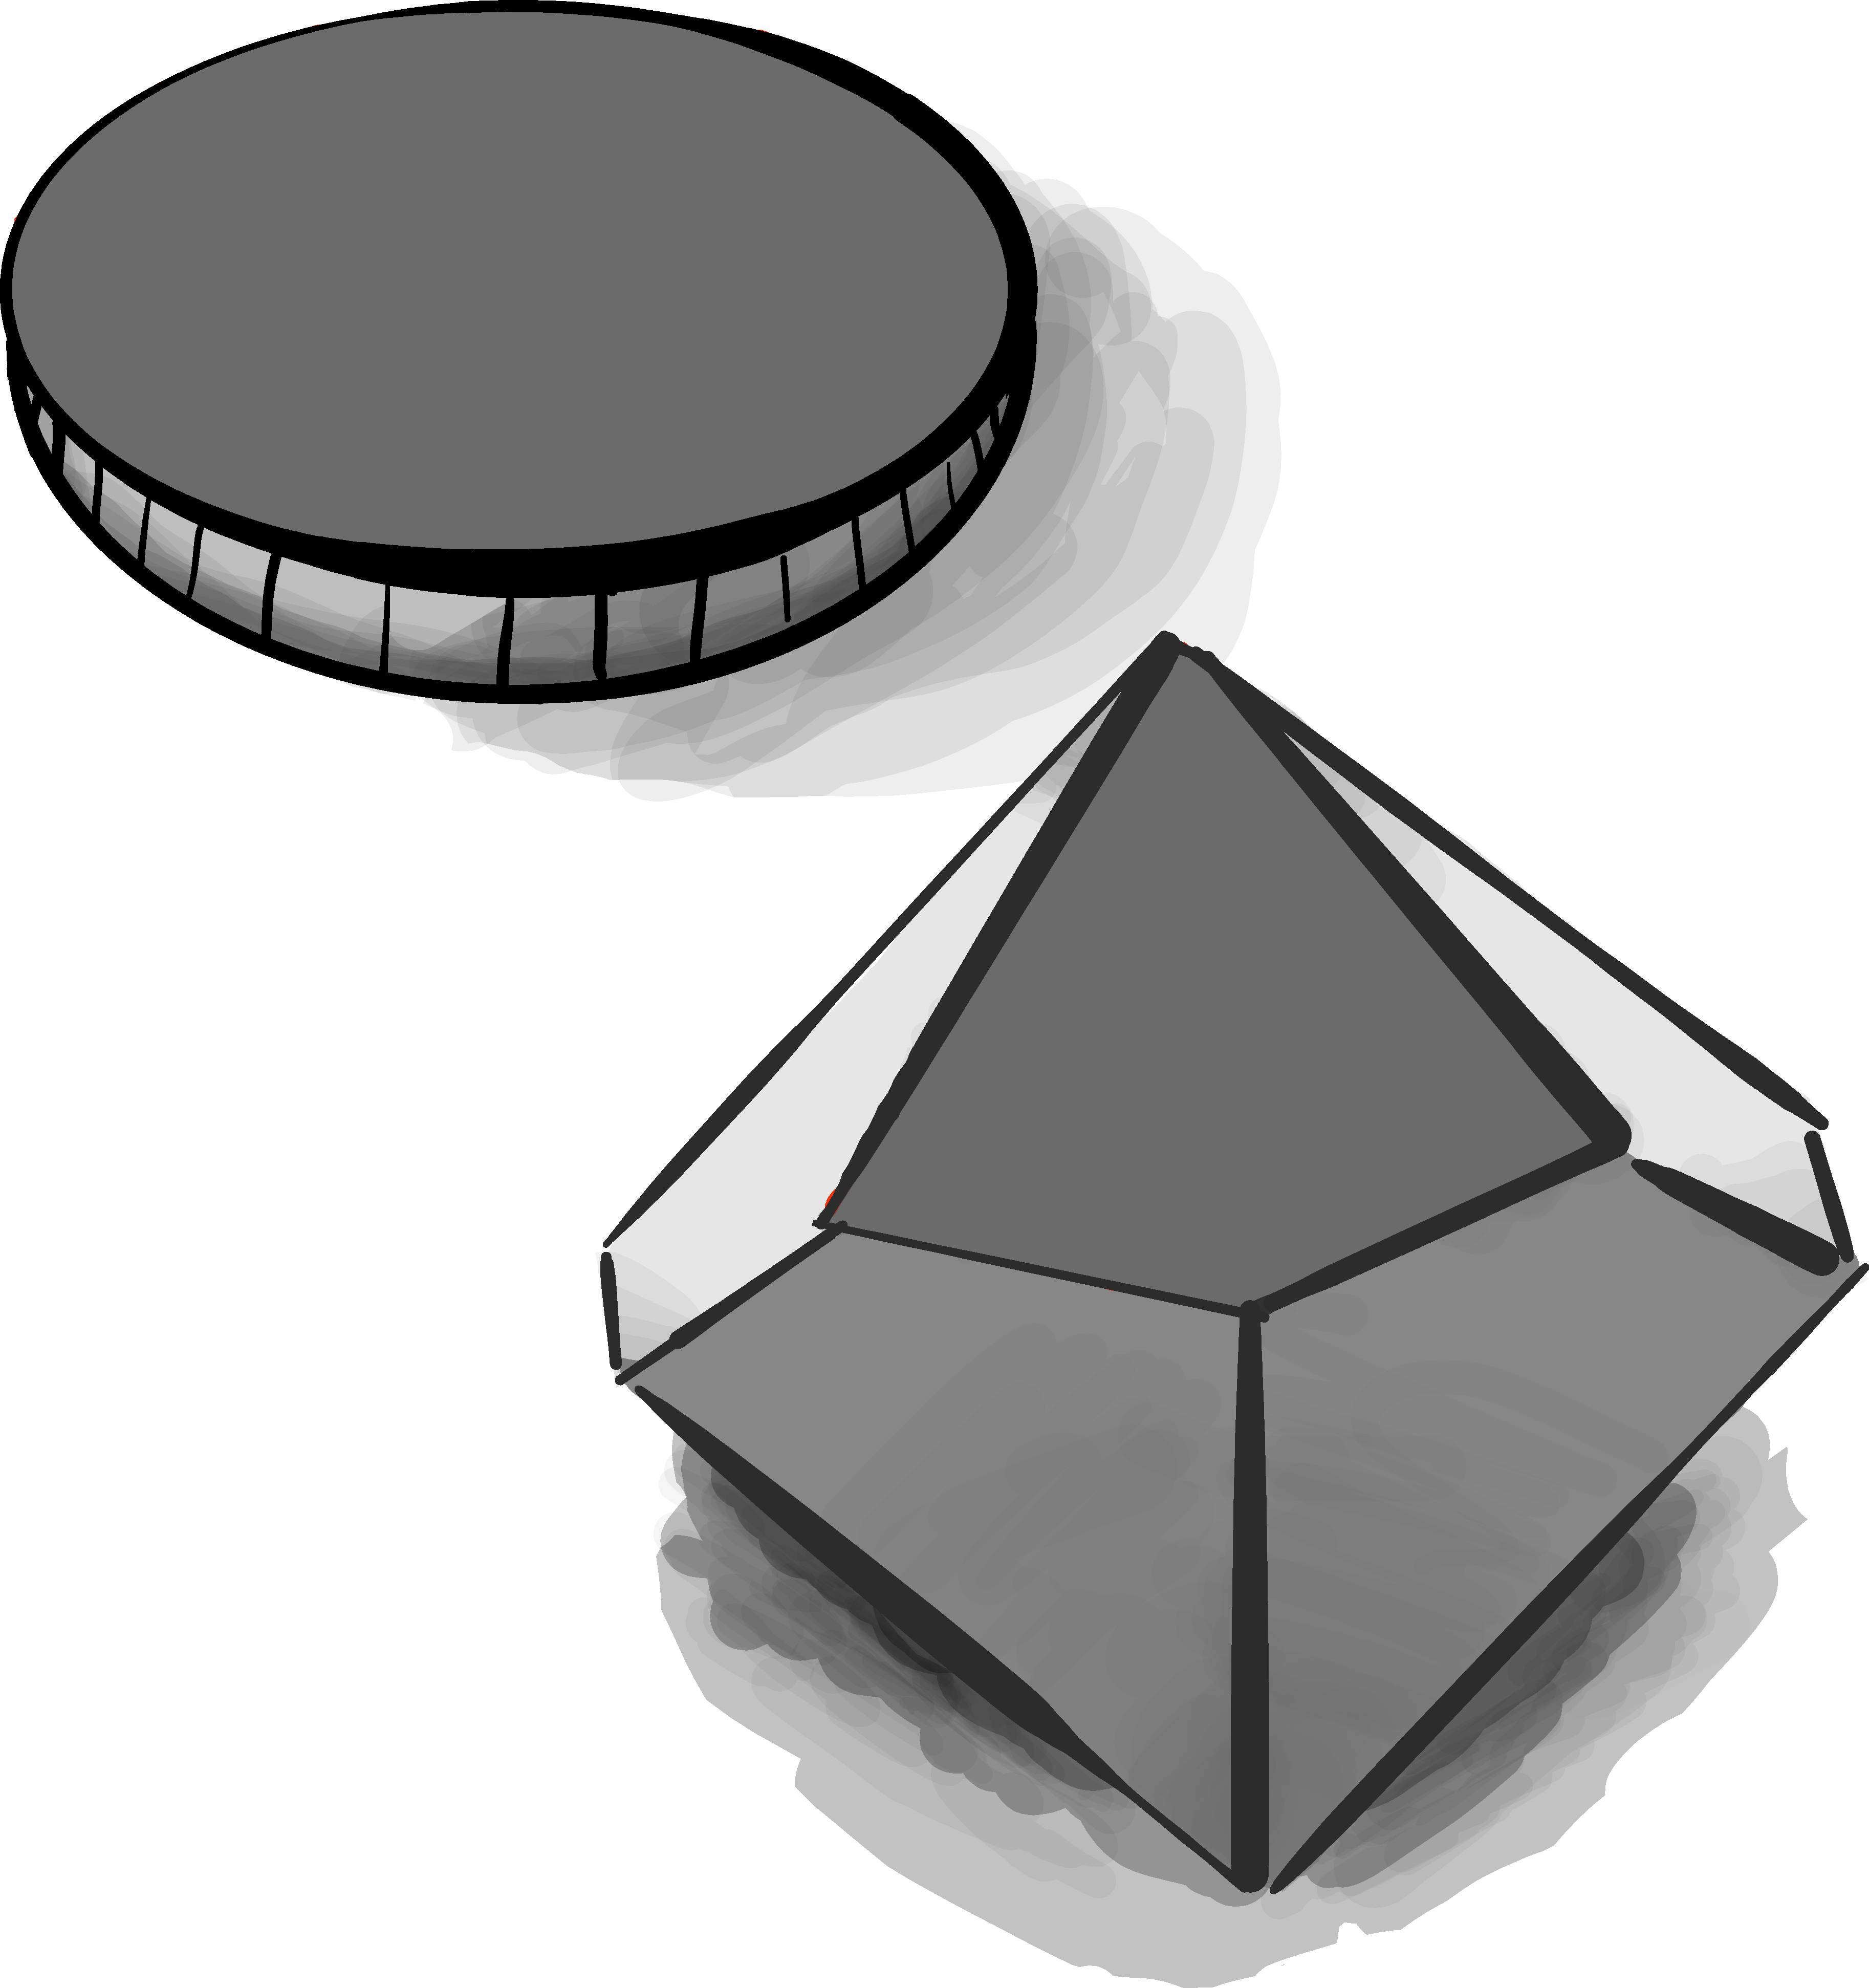
\includegraphics[trim= 0 0 0 -20ex, clip, width=0.3\textwidth]{img/grey-coin-grey-die} \\ $\bm{A} = \text{``grey coin, grey die''}$}
\end{tabular}
\end{center}

Because the die and the coin are independent, it is straightforward to calculate the probability of each of the four possible states of the big box.
For example, to compute the probability that the die and the coin are both grey side up we calculate,
\begin{align*}
p_{\bm{A} = \text{``grey coin, grey die''}}
&= p_{\bm{C} = \text{grey}} \times p_{\bm{D} = \text{grey}} \\
&= 0.5 \times 0.9 \\
&= 0.45.
\end{align*}
The probabilities of all four possible states of the big box are summarized below.
\begin{center}
 \begin{tabular}{c c || c | c || c}
 \multicolumn{2}{c}{\multirow{2}{*}{$\bm{A}$}} & \multicolumn{2}{c}{$\bm{C}$} & {}\\
\multicolumn{2}{c}{} & red & grey & sum \\ [0.5ex]
 \hline\hline
\multirow{2}{*}{$\bm{D}$} & red & 0.05 & 0.05 & 0.1 \\
 \cline{2-5}
 & grey & 0.45 & 0.45 & 0.9 \\
 \hline\hline
  {} & sum & 0.5 & 0.5 & 1 \\ [1ex]
\end{tabular}
\end{center}

Now that we know the probabilities for all the possible outcomes of $\bm{A}$, we can calculate the entropy associated with the the closed box.
\begin{align*}
S_{\text{big box}}
&=
H(\bm{A}) \\
&=
- 0.05 \times \log_2(0.05)
+ - 0.05 \times \log_2(0.05)
- 0.45 \times \log_2(0.45)
+ - 0.45 \times \log_2(0.45) \\
&\approx 1.469
\end{align*}

Let's take a moment to notice,
\begin{align*}
S_{\text{big box}}
&=
S_{\text{die}} + S_{\text{coin}}.
\end{align*}

Intuitively, it makes sense that the entropy associated with the big box is the same as the sum of the entropy associated with the die box and the entropy associated with the coin box.
This relation holds true because the coin and the die are independent.
Intuitively speaking, the coin and the die are independent because knowing the state of the coin doesn't the probability of outcomes from the die and vice versa.
\begin{center}
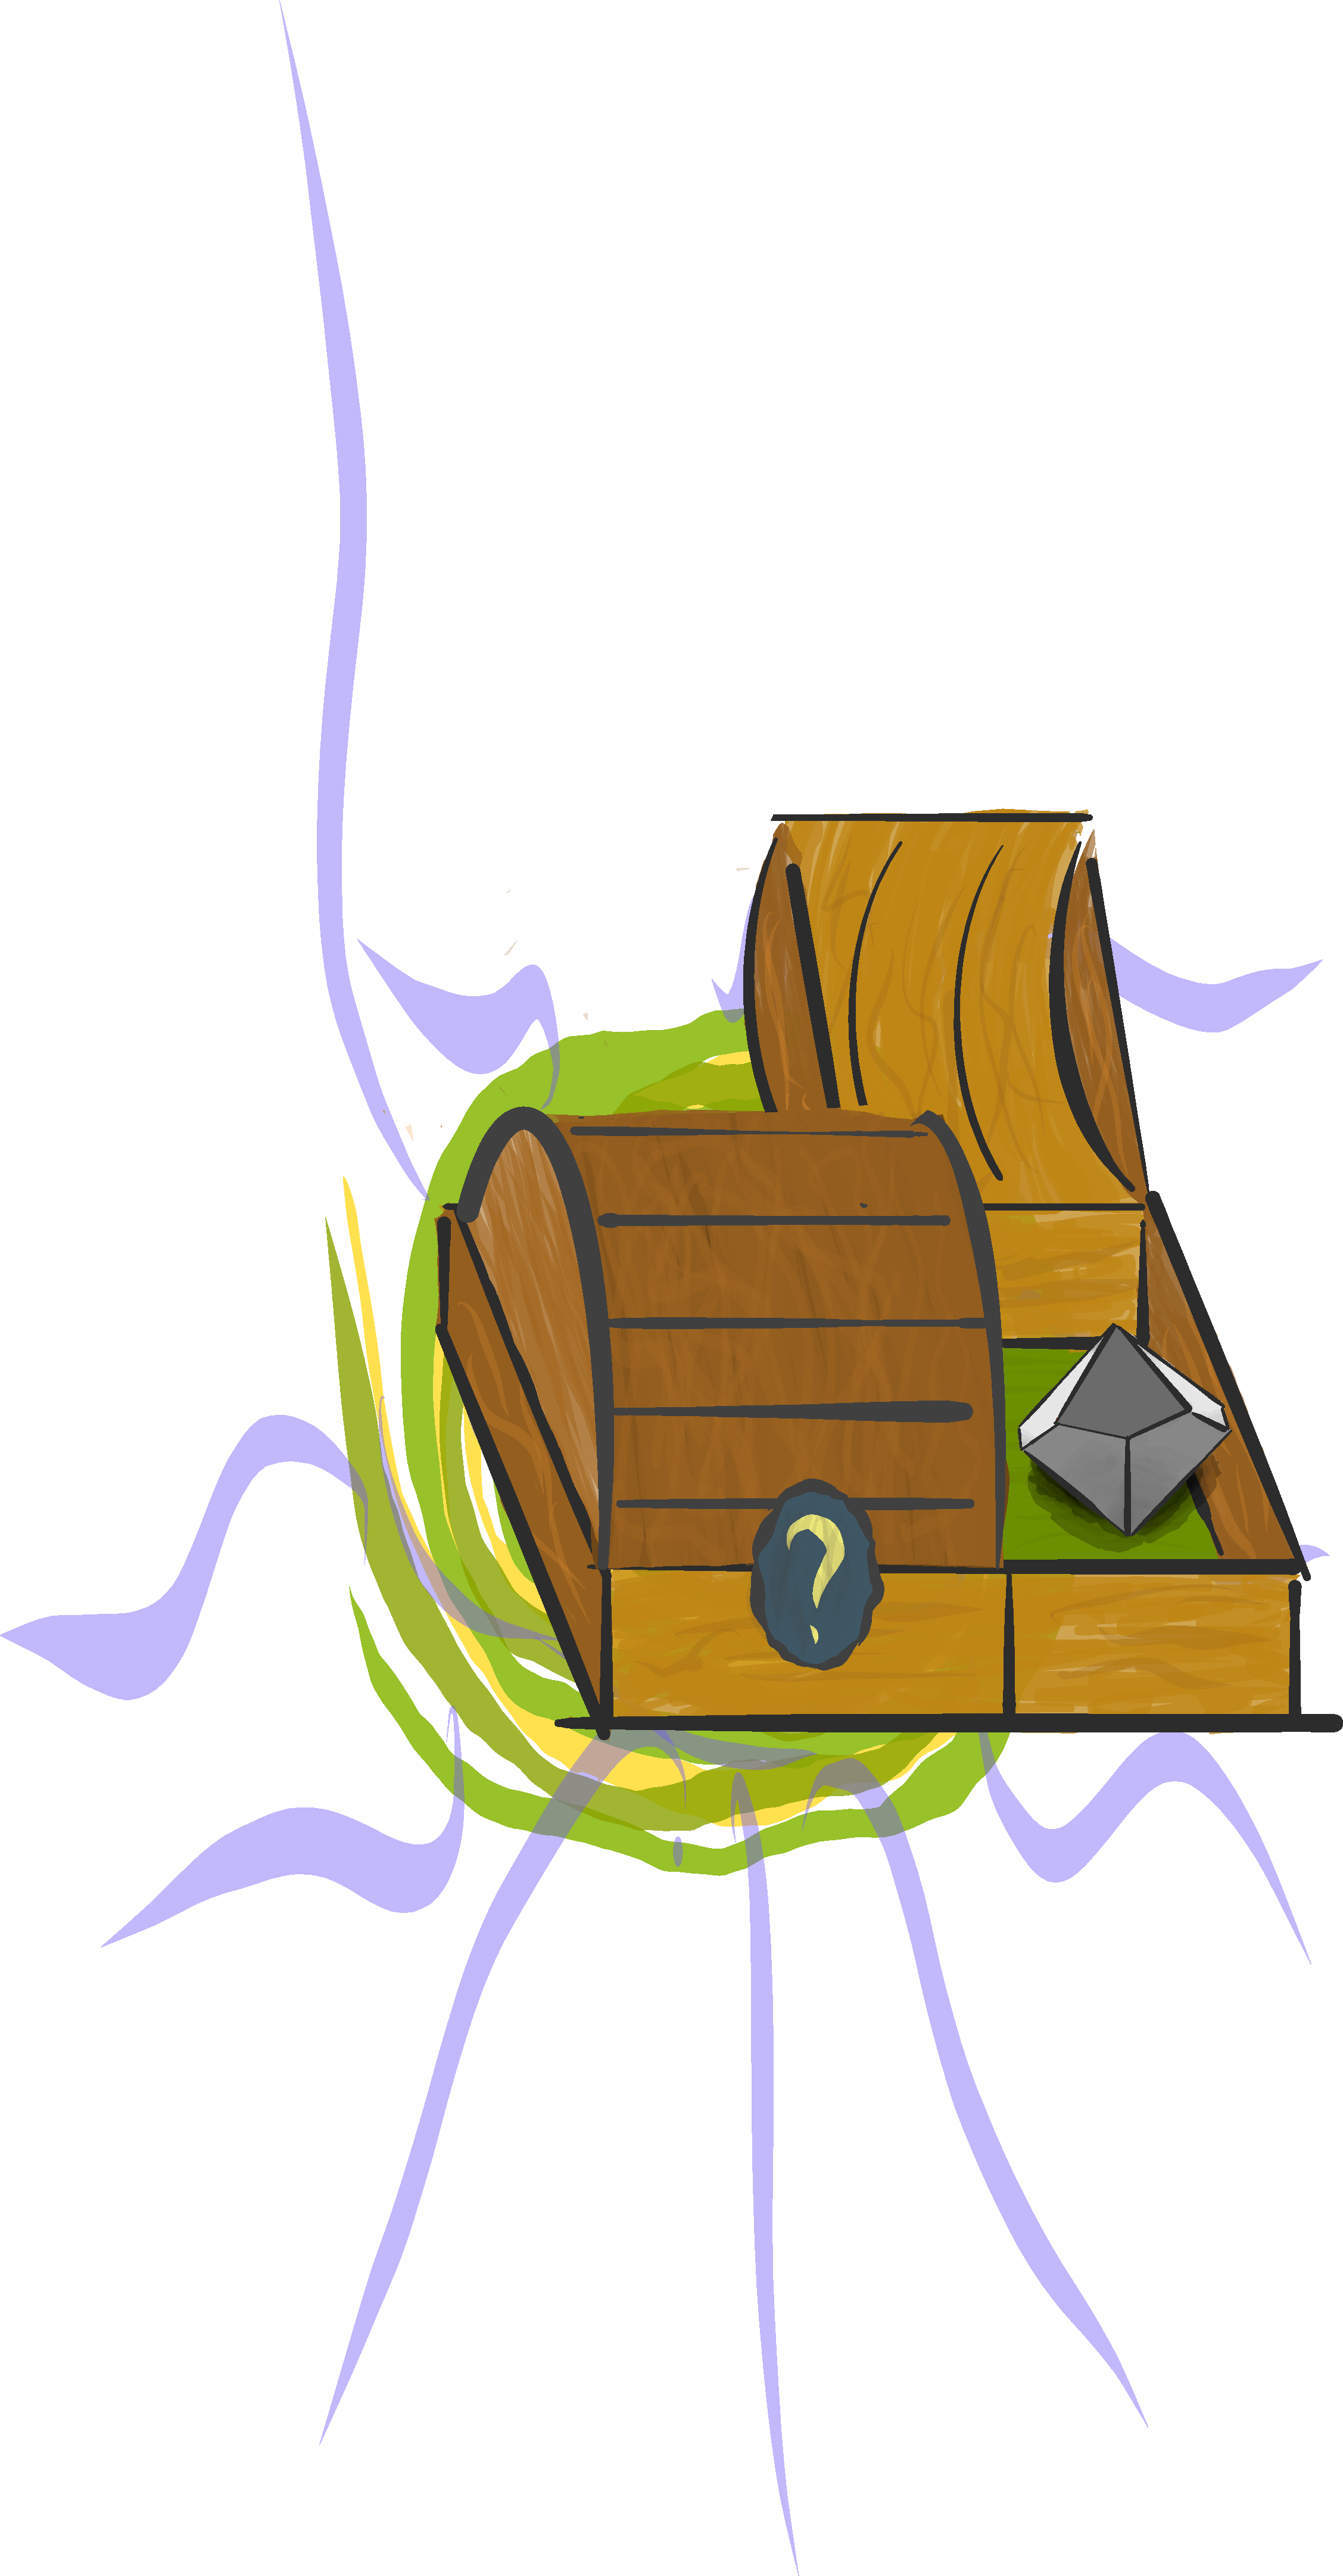
\includegraphics[width=0.3\textwidth]{img/left-box-closed-portal-die}
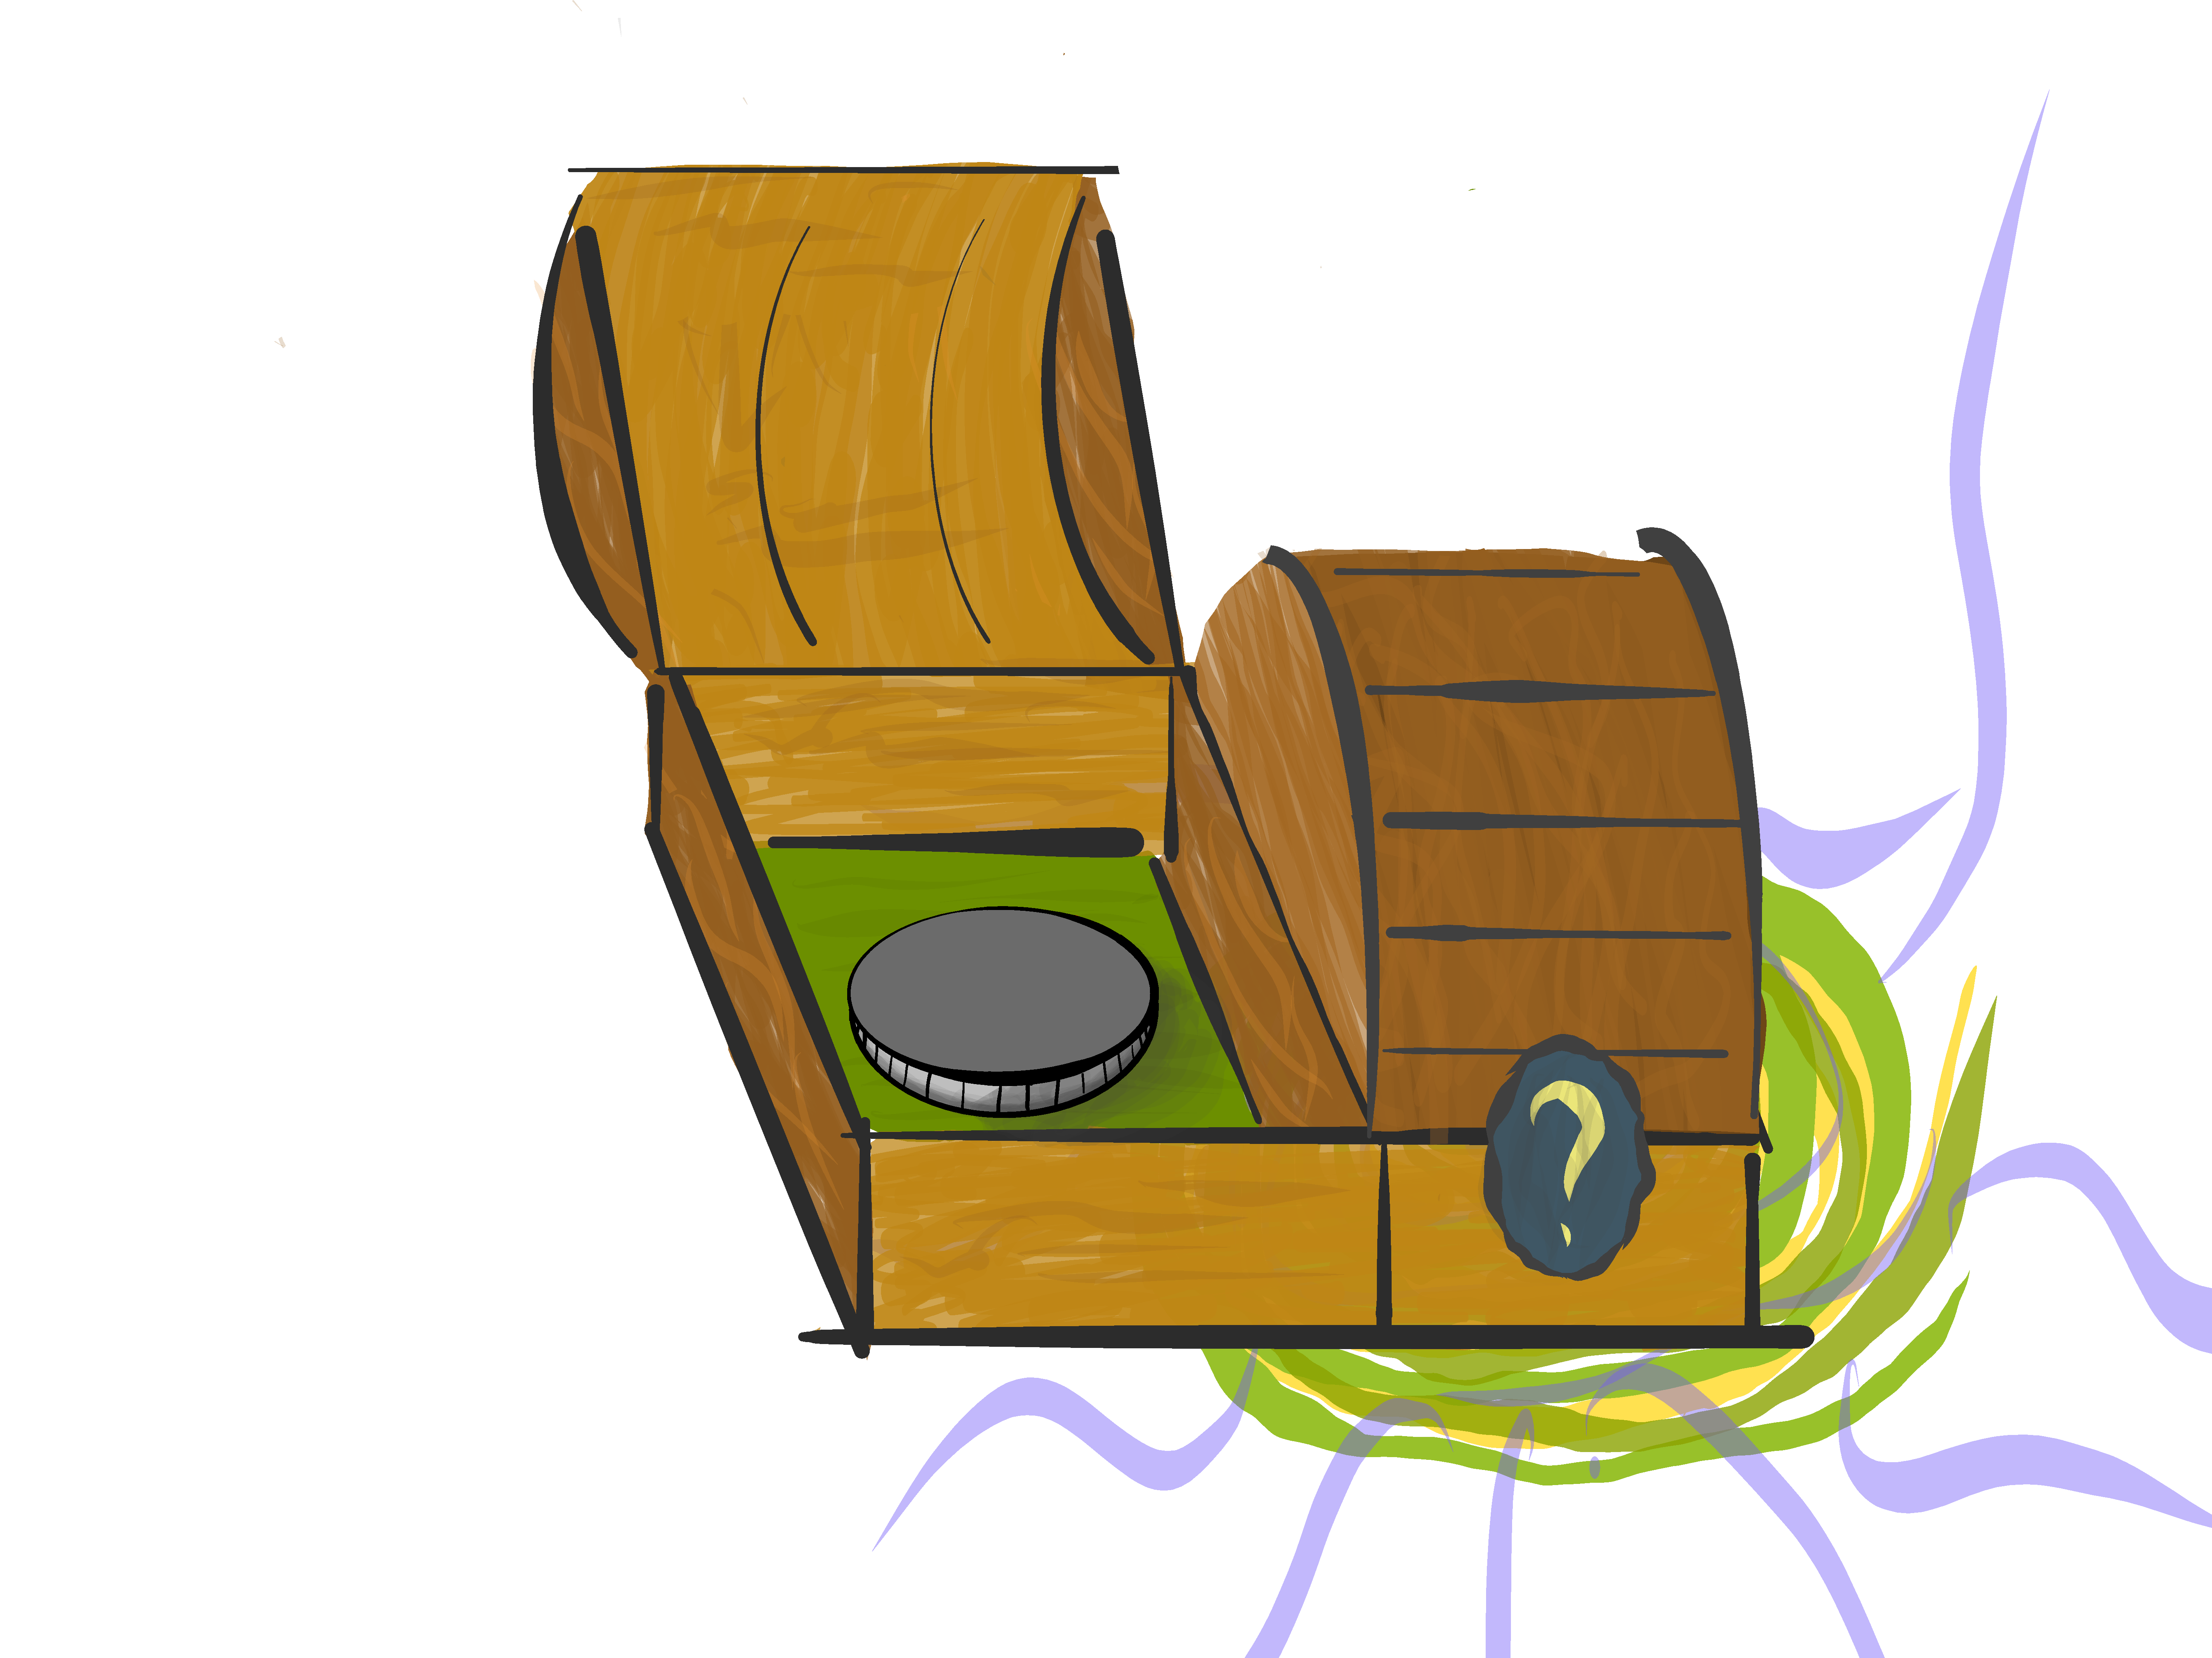
\includegraphics[trim= 0 -200ex 0 0, clip,width=0.4\textwidth]{img/right-box-closed-portal-coin}
\end{center}
The coin still has the same probability of taking on the red state or grey state given we know the state of the die.
The die still has the same probability of taking on the red state or grey state given we know the state of the coin.
Mathematically,
\begin{align*}
P(\bm{C}) &= P(\bm{C} | \bm{D}) \\
P(\bm{D}) &= P(\bm{D} | \bm{C}) .
\end{align*}
For those unfamiliar, the vertical bar is read as ``given.''

In the next section, we'll look at entropy and information in a situation where independence \textit{doesn't} hold.
This is where things get a little more interesting.


\section{Dependent Random Variables}

Let's put our die and coin away to step outside.
To look at dependent random variables, we will consider a hypothetical weather scenario.
We will consider two aspects of the weather: precipitation and light.
In our hypothetical scenario, precipitation conditions may either be dry or wet.
We will model the situation with a random variable $\bm{P}$ that can take on the value ``dry'' or ``wet.''
The probability that conditions are dry is 0.9 and the probability that conditions are wet is 0.1.
\begin{center}
  \begin{tabular}{c c}
  \makecell{
    
\includegraphics[width=0.5\textwidth]{img/dry} \\
    $p_{\bm{P} = \text{dry}} = 0.9$
    }
  &
  \makecell{
    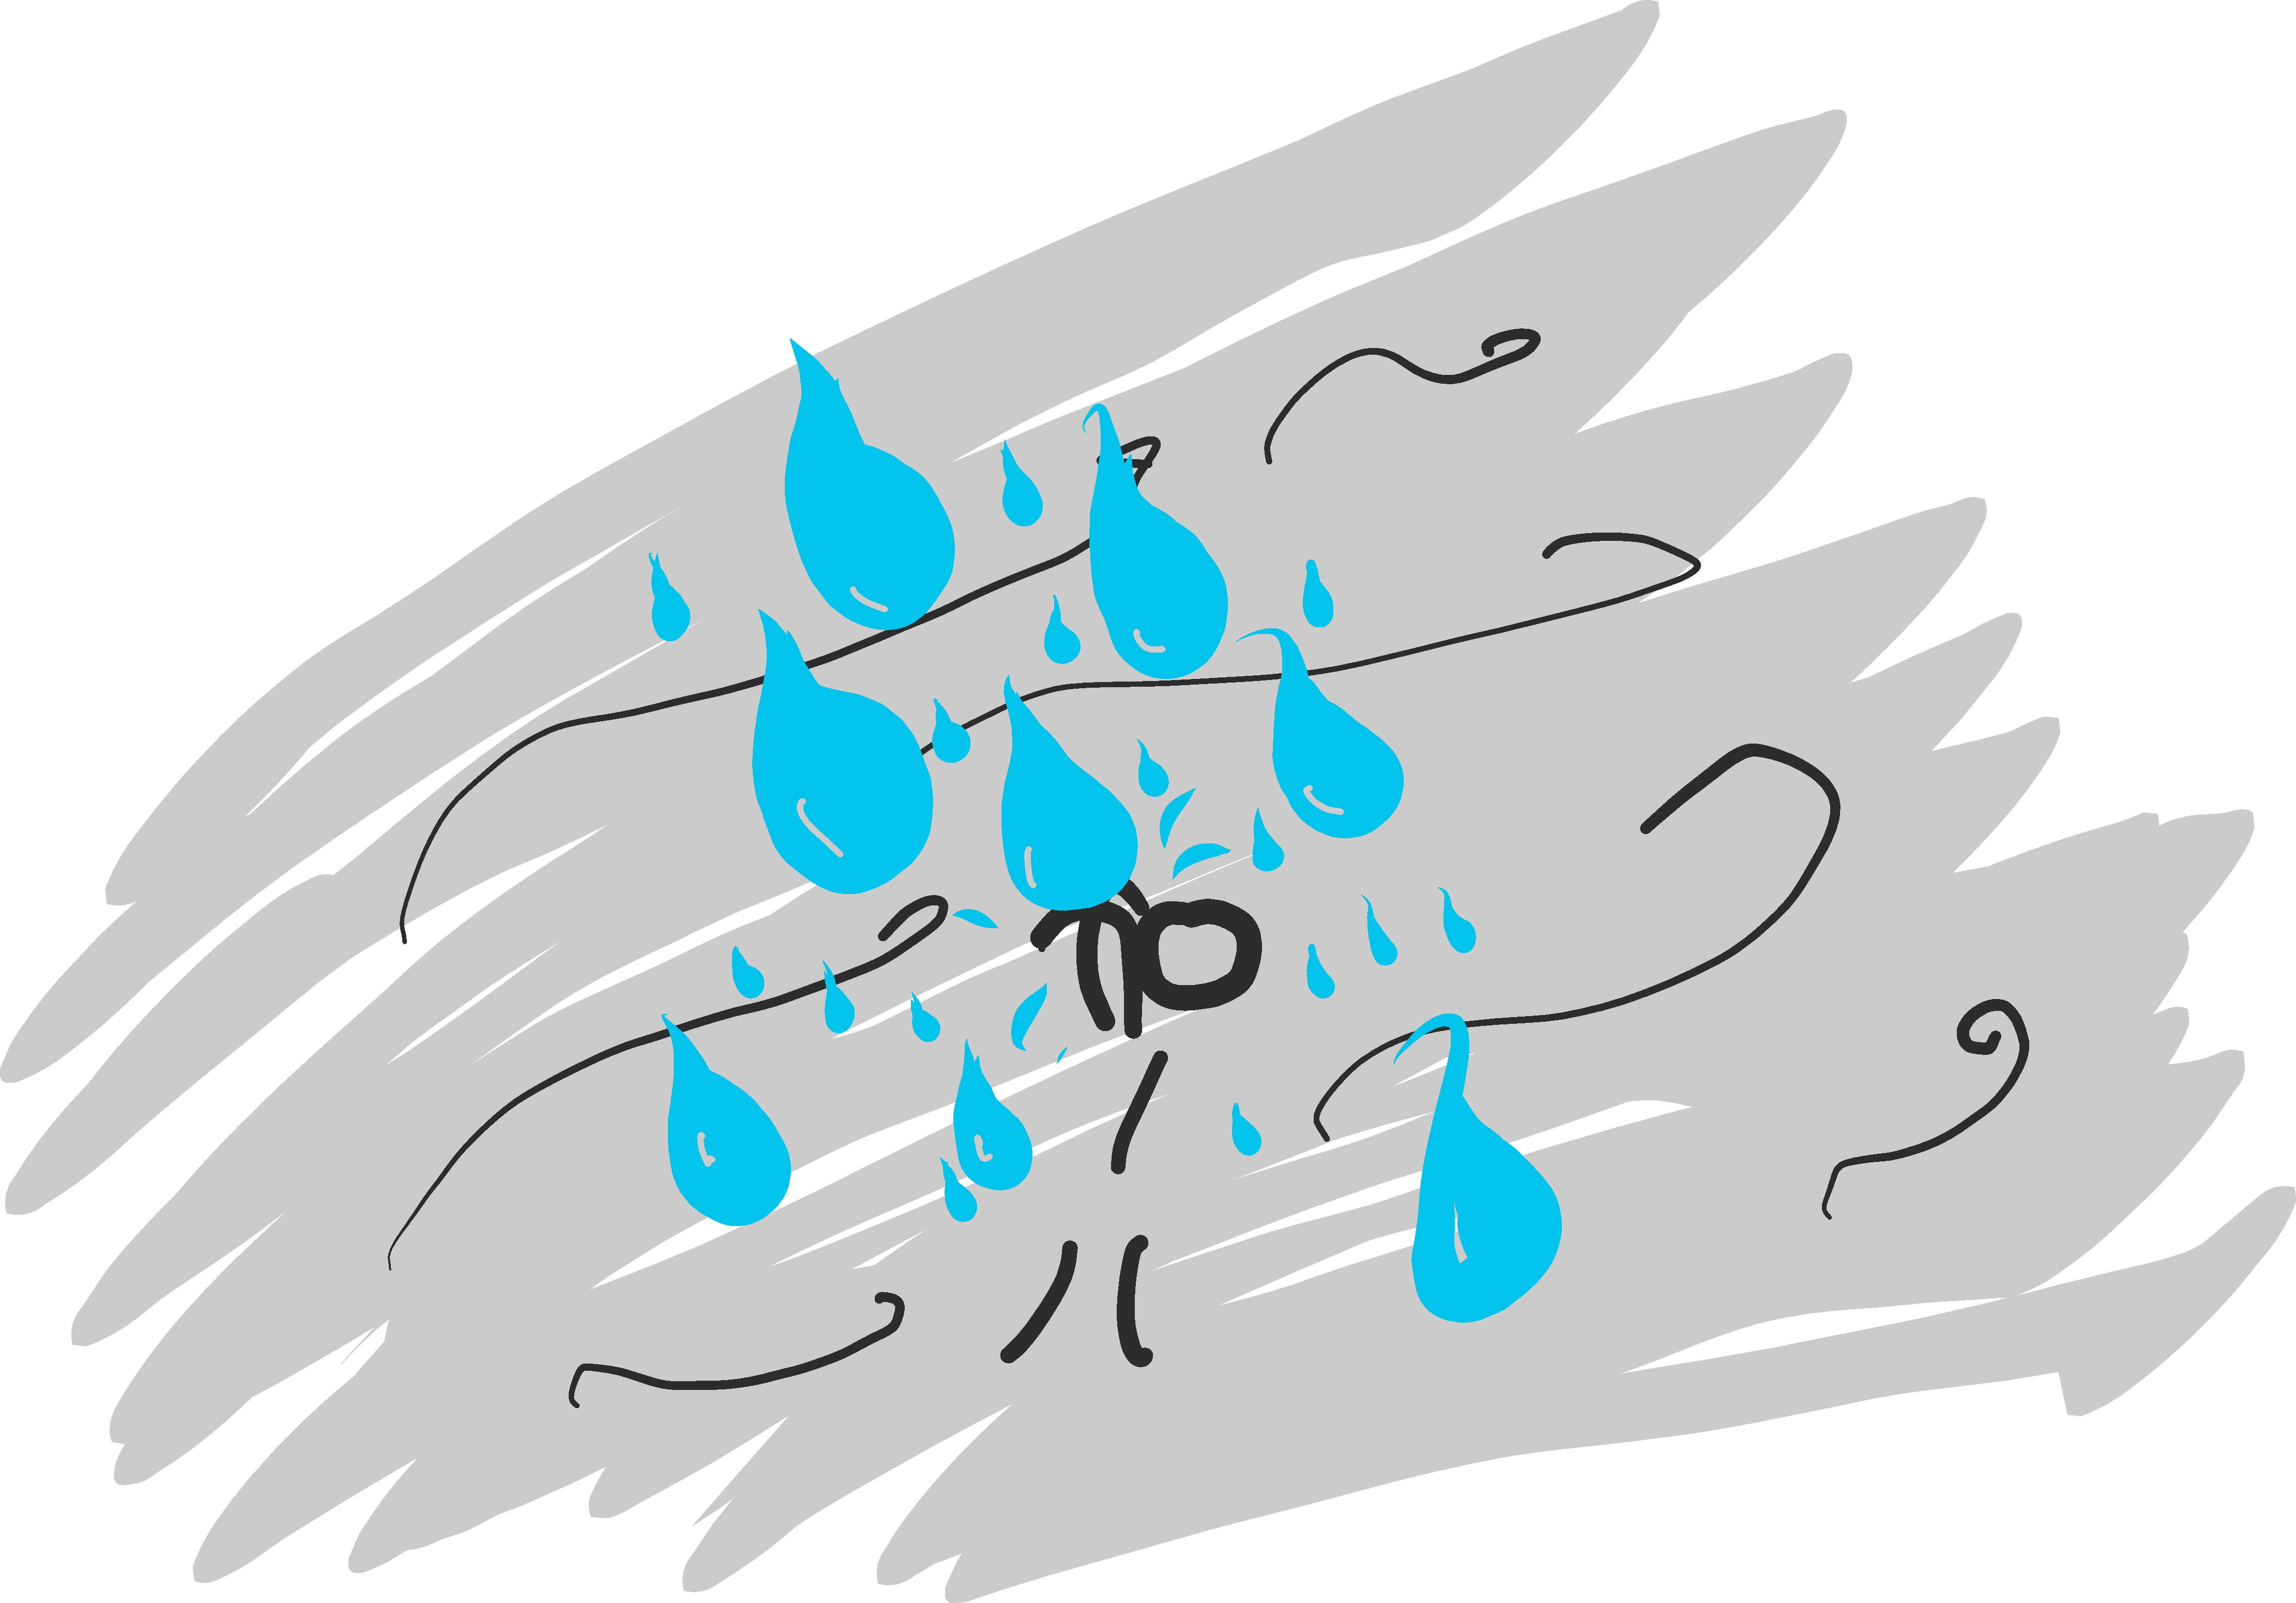
\includegraphics[width=0.3\textwidth]{img/rain} \\
    $p_{\bm{P} = \text{wet}} = 0.1$
    }
  \end{tabular}
\end{center}
Similarly, we model light conditions with a random variable $\bm{L}$ that can take on the value ``sunny'' or ``overcast.''
Sunny means that clouds are not currently occluding the sun (but may be present elsewhere in the sky).
Overcast means that the sun is currently occluded by cloud cover.
The probability that conditions are sunny is 0.5 and the probability that conditions are wet is 0.5.
\begin{center}
  \begin{tabular}{c c}
  \makecell{
    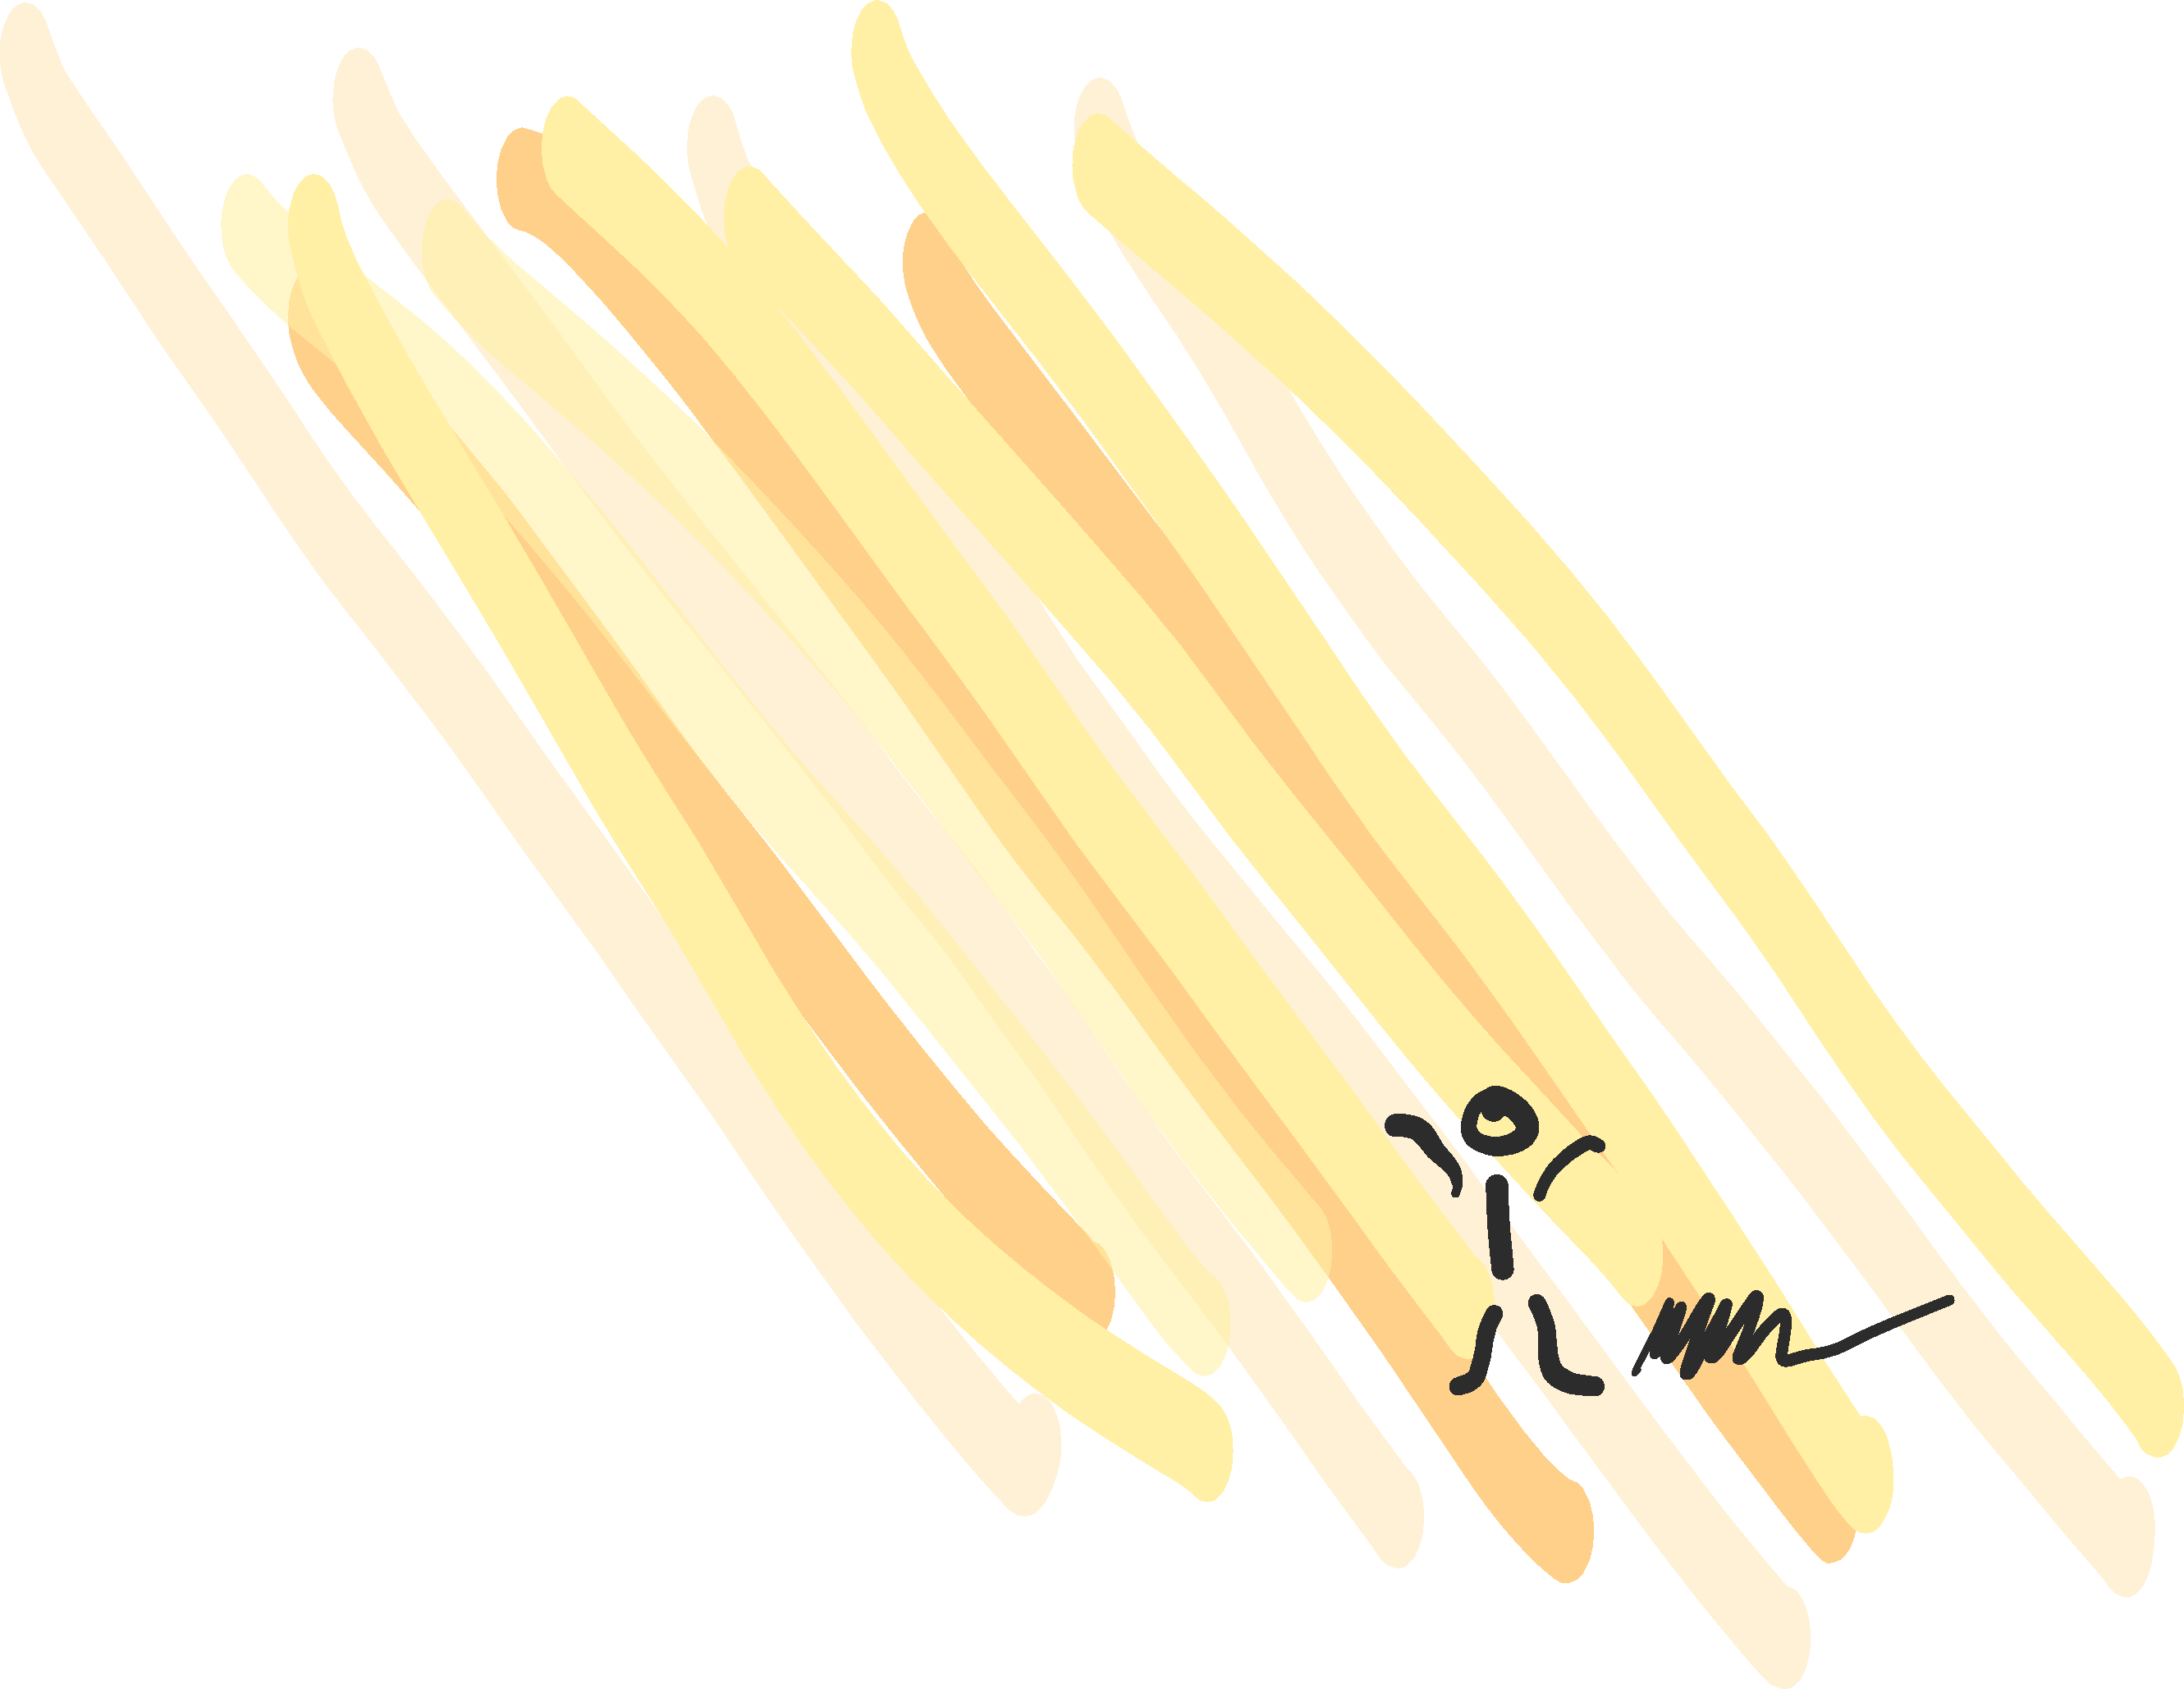
\includegraphics[width=0.3\textwidth]{img/sun} \\
    $p_{\bm{P} = \text{dry}} = 0.5$
    }
  &
  \makecell{
    
\includegraphics[width=0.3\textwidth]{img/cloud} \\
    $p_{\bm{P} = \text{wet}} = 0.5$
    }
  \end{tabular}
\end{center}

This setup looks familiar.
In the coin and die scenario, we had a pair of random variables that could each take on two values.
One random variable takes on each of its values with probability $\frac{1}{2}$.
the other random variable takes on one of its values with probability $\frac{9}{10}$ and the other with probability $\frac{1}{10}$.

The key difference is that precipitation and light are not independent.
Intuitively, we expect the wet and overcast conditions to be correlated and the dry and sunny conditions to be correlated.
For example, if it's raining we would be very surprised if it was sunny!

Let's look at how precipitation and light interact in our hypothetical scenario.
We will model the weather --- the combination of precipitation and light --- as a single random variable $\bm{W}$.
The weather can be in four possible states,
\begin{center}
 \begin{tabular}{c c || c | c }
 \multicolumn{2}{c}{\multirow{2}{*}{$\bm{W}$}} & \multicolumn{2}{c}{$\bm{P}$} \\
\multicolumn{2}{c}{} & rainy & dry \\ [0.5ex]
 \hline\hline
\multirow{10}{*}{$\bm{L}$} & sunny
& \makecell{
  
\includegraphics[trim= 0 0 0 0, clip, width=0.3\textwidth]{img/sun-rain} \\
  $\bm{W} = \text{``rainy, sunny''}$
  }
 & \makecell{
  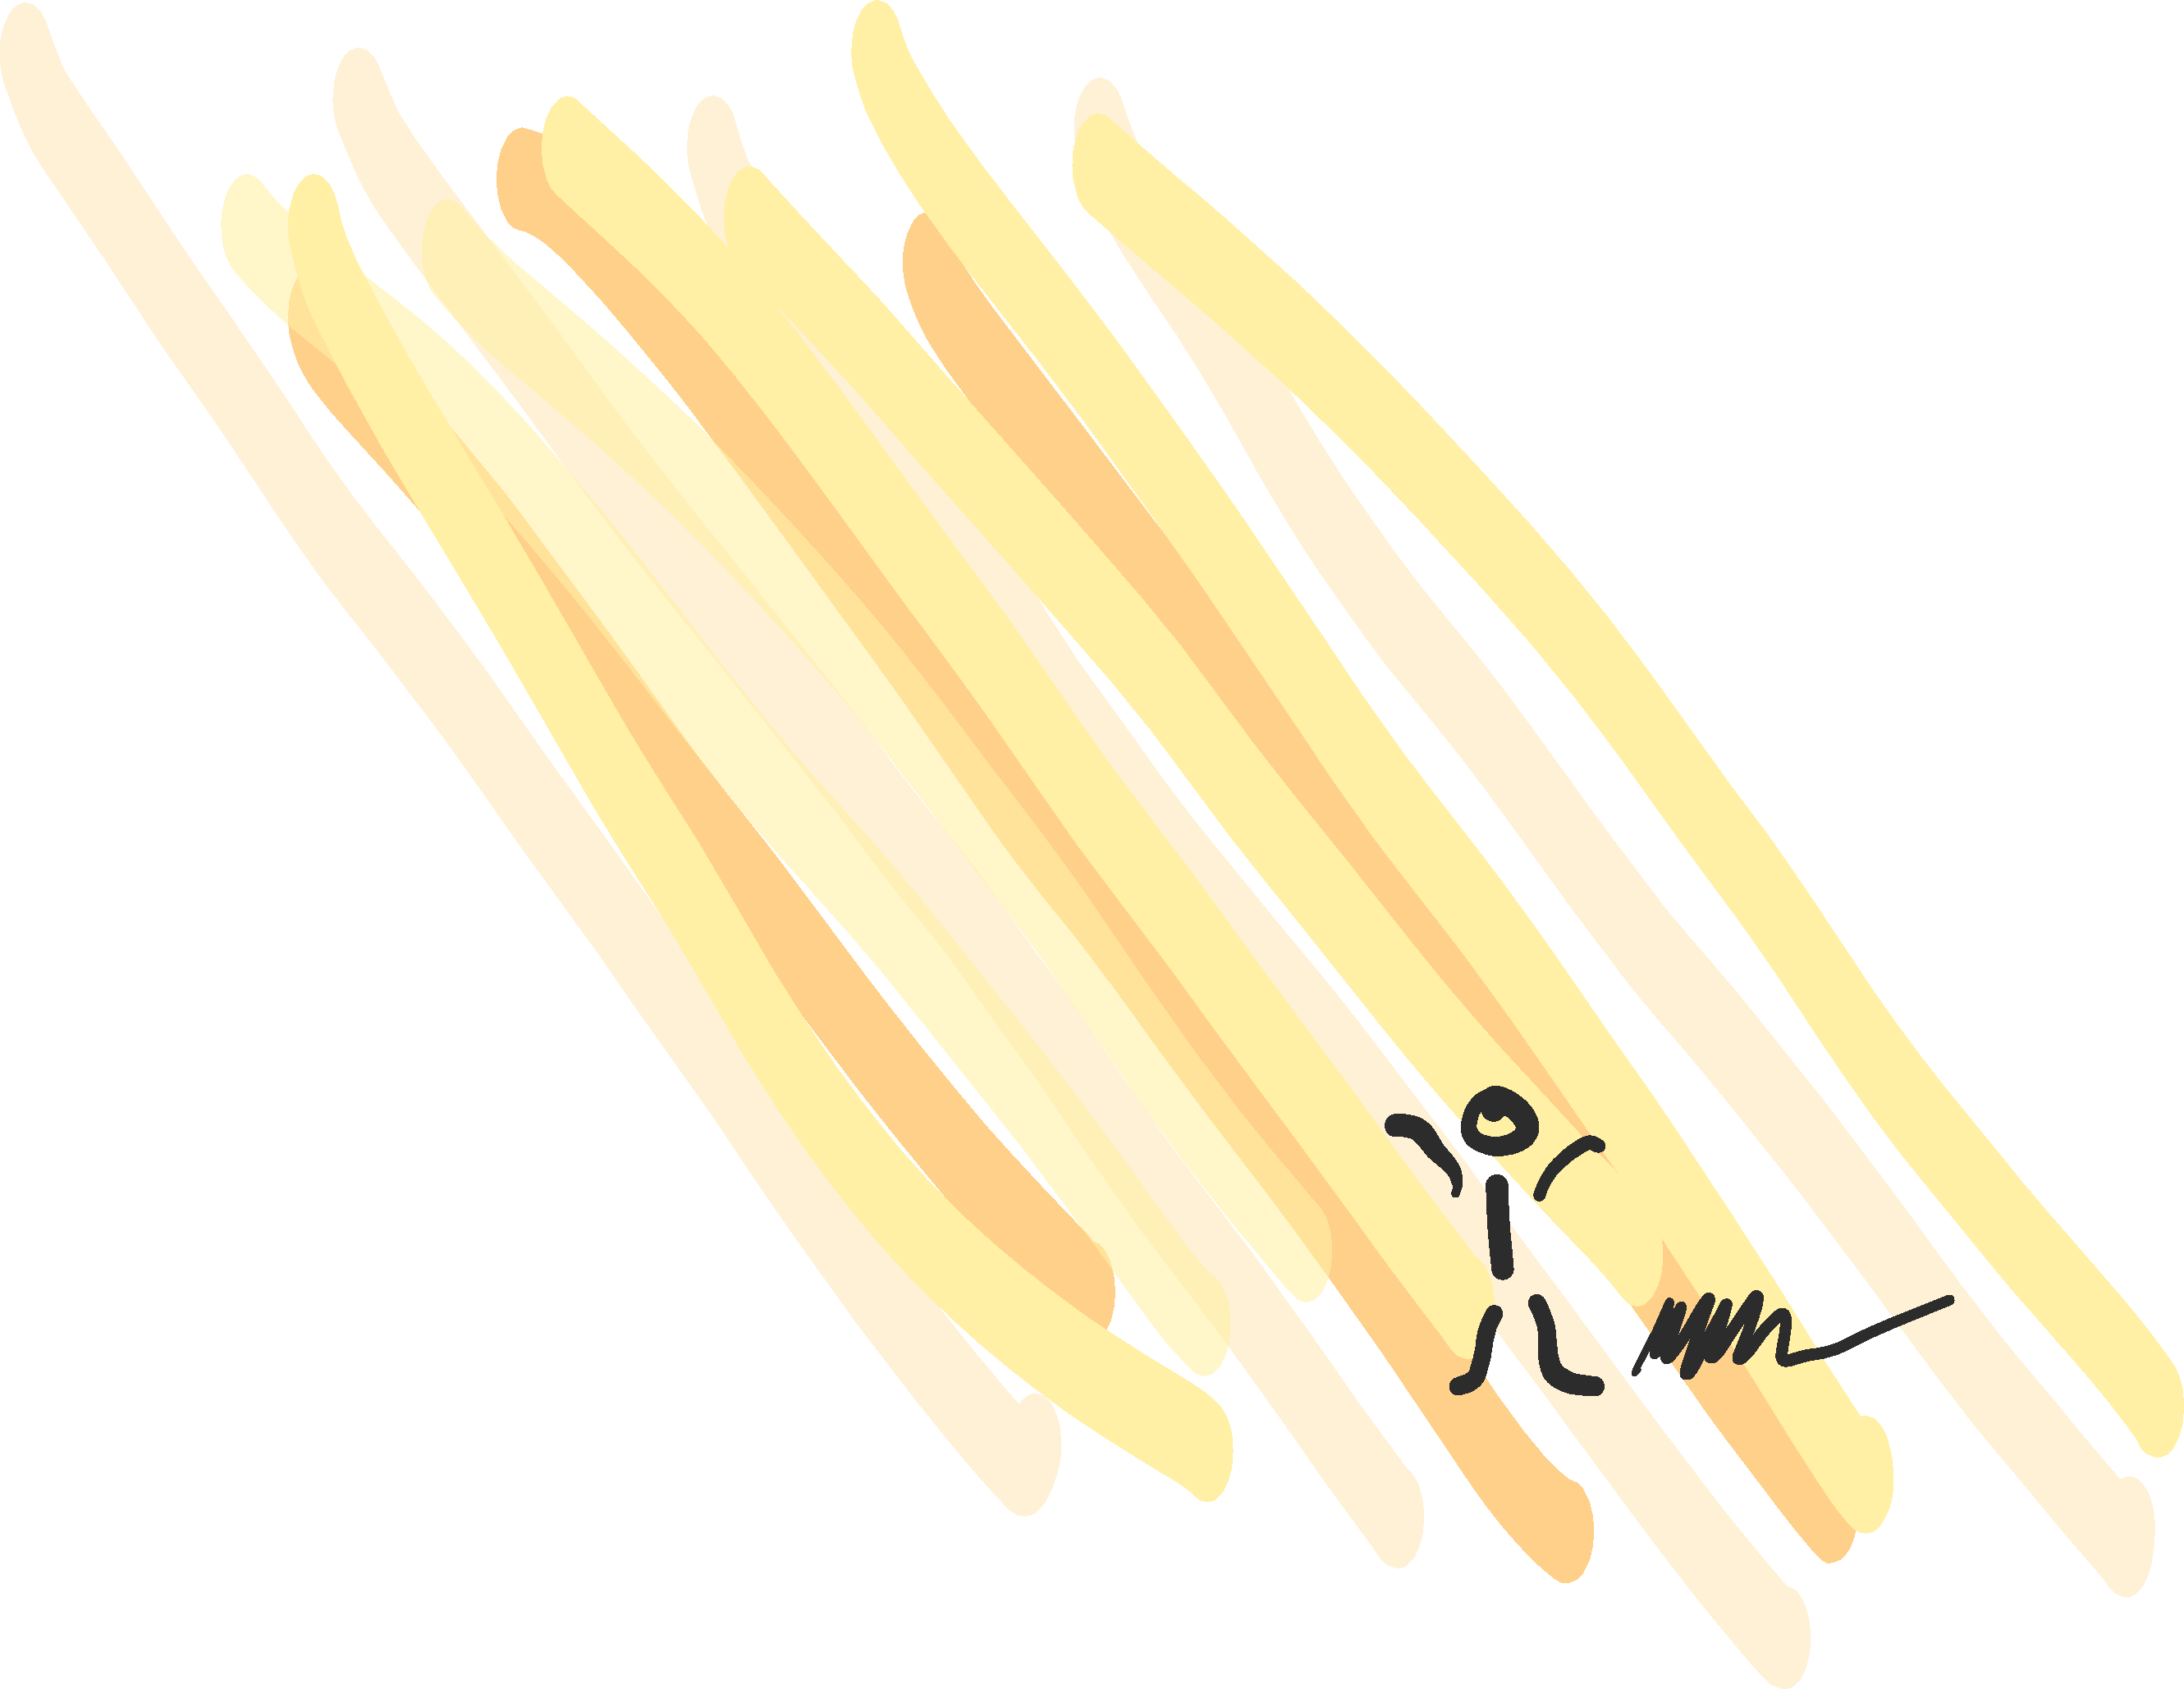
\includegraphics[trim= 0 0 0 0, clip, width=0.3\textwidth]{img/sun} \\
  $\bm{W} = \text{``dry, sunny''}$
  }
  \\
 \cline{2-4}
 & overcast
 & \makecell{
 
\includegraphics[trim= 0 0 0 0, clip, width=0.3\textwidth]{img/cloud-rain} \\
  $\bm{W} = \text{``rainy, overcast''}$}
 & \makecell{
 
\includegraphics[trim= 0 0 0 0, clip, width=0.3\textwidth]{img/cloud} \\ $\bm{W} = \text{``dry, overcast''}$}
\end{tabular}
\end{center}

Because we are no longer operating under the assumption of independence, the probabilities of the four states of $\bm{W}$ can no longer be derived from the probability distributions of $\bm{P}$ (precipitation) and $\bm{L}$ (light).
Just as we took it at face value that in our scenario the probability of the sunny and cloudy condition are both $\frac{1}{2}$, we take the probability of each of the four possible states of $\bm{W}$ at face value as describing the particular scenario we are imagining.
(Of course, this is under the constraint that the marginal probabilities of $\bm{P}$ and $\bm{L}$ are consistent with what we stated before).
Let's define the probability distribution of $\bm{W}$ as follows,
\begin{center}
 \begin{tabular}{c c || c | c || c}
 \multicolumn{2}{c}{\multirow{2}{*}{$\bm{W}$}} & \multicolumn{2}{c}{$\bm{L}$} & {}\\
\multicolumn{2}{c}{} & sunny & overcast & sum \\ [0.5ex]
 \hline\hline
\multirow{2}{*}{$\bm{P}$} & wet & 0.005 & 0.095 & 0.1 \\
 \cline{2-5}
 & dry & 0.495 & 0.405 & 0.9 \\
 \hline\hline
  {} & sum & 0.5 & 0.5 & 1 \\ [1ex]
\end{tabular}.
\end{center}

The best way to get a feel for the distribution of $\bm{W}$ is to look at conditional probabilities.
For example, here's the probability that we observe the sunny weather given we know that it's wet outside,
\begin{align*}
P(\bm{L} = \text{sunny} | \bm{P} = \text{wet}) &= 0.05.
\end{align*}

Although we won't elaborate on it, calculating such conditional probabilities from the table above is very straightforward.
Let's look through the rest of the rest of the conditional probabilities we can calculate.

Consider
\begin{align*}
  P(\bm{L} = \text{sunny} | \bm{P} = \text{dry}) &= 0.55 \\
  P(\bm{L} = \text{sunny}) &= 0.5 \\
  P(\bm{L} = \text{sunny} | \bm{P} = \text{wet}) &= 0.05.
\end{align*}
Here, we see that the probability of observing sunny weather is greatest if we know that it's dry outside and very small if we know that it's wet outside.

Likewise,
\begin{align*}
P(\bm{L} = \text{overcast} | \bm{P} = \text{wet}) &= 0.95 \\
P(\bm{L} = \text{overcast}) &= 0.5 \\
P(\bm{L} = \text{overcast} | \bm{P} = \text{dry}) &= 0.45.
\end{align*}
The probability of observing overcast weather is greatest if we know that it's wet outside and less if we know that it's dry outside.

Similarly,
\begin{align*}
P(\bm{P} = \text{wet} | \bm{L} = \text{overcast}) &= 0.19 \\
P(\bm{P} = \text{wet}) &= 0.1 \\
P(\bm{P} = \text{wet} | \bm{L} = \text{sunny}) &= 0.01.
\end{align*}
The probability of observing wet weather is greatest if we know it's overcast outside and least if we know it's sunny outside.

Finally,
\begin{align*}
P(\bm{P} = \text{dry} | \bm{L} = \text{sunny}) &= 0.99 \\
P(\bm{P} = \text{dry}) &= 0.9 \\
P(\bm{P} = \text{dry} | \bm{L} = \text{overcast}) &= 0.81.
\end{align*}
The probability of observing dry weather is greatest if we know it's sunny outside and least if we know it's overcast.

Armed with a good understanding of the probability distribution of our weather $\bm{W}$, we're ready to talk entropy and information.
We can calculate entropy of a random variable whose distribution we know using Equation \ref{eqn:shannon}.
Let's do that for $\bm{W}$,
\begin{align*}
S_{\text{weather}}
&=
H(\bm{W}) \\
&=
- 0.005 \times \log_2(0.005)
+ - 0.095 \times \log_2(0.095)
- 0.495 \times \log_2(0.495)
+ - 0.405 \times \log_2(0.405) \\
&\approx 1.391
\end{align*}
for $\bm{L}$,
\begin{align*}
  S_{\text{light}}
  &=
  H(\bm{L}) \\
  &=
  - 0.5 \times \log_2(0.5)
  + - 0.5 \times \log_2(0.5) \\
  &= 1
\end{align*}
and, finally, for $\bm{P}$,
\begin{align*}
  S_{\text{precipitation}}
  &=
  H(\bm{P}) \\
  &=
  - 0.1 \times \log_2(0.1)
  + - 0.9 \times \log_2(0.9) \\
  &\approx 0.469.
\end{align*}

Just like for the die and the coin, $S_{\text{light}} > S_{\text{precipitation}}$.
Like before, this makes sense because we can make a better guess about precipitation (it is wet infrequently) than about light conditions (it is overcast or sunny with equal probability).

Here's the shocker,
\begin{align*}
S_{\text{weather}}
\not{=}
S_{\text{light}} + S_{\text{precipitation}}
\end{align*}
In fact, $1.391 < 1.469$, so
\begin{align*}
S_{\text{weather}}
<
S_{\text{light}} + S_{\text{precipitation}}.
\end{align*}
How can our uncertainty about the weather as an entire system be less than our uncertainty about its constituent parts?
The answer is that some entropy is shared between $\bm{L}$ and $\bm{P}$.
The situation looks like this.
\begin{center}
  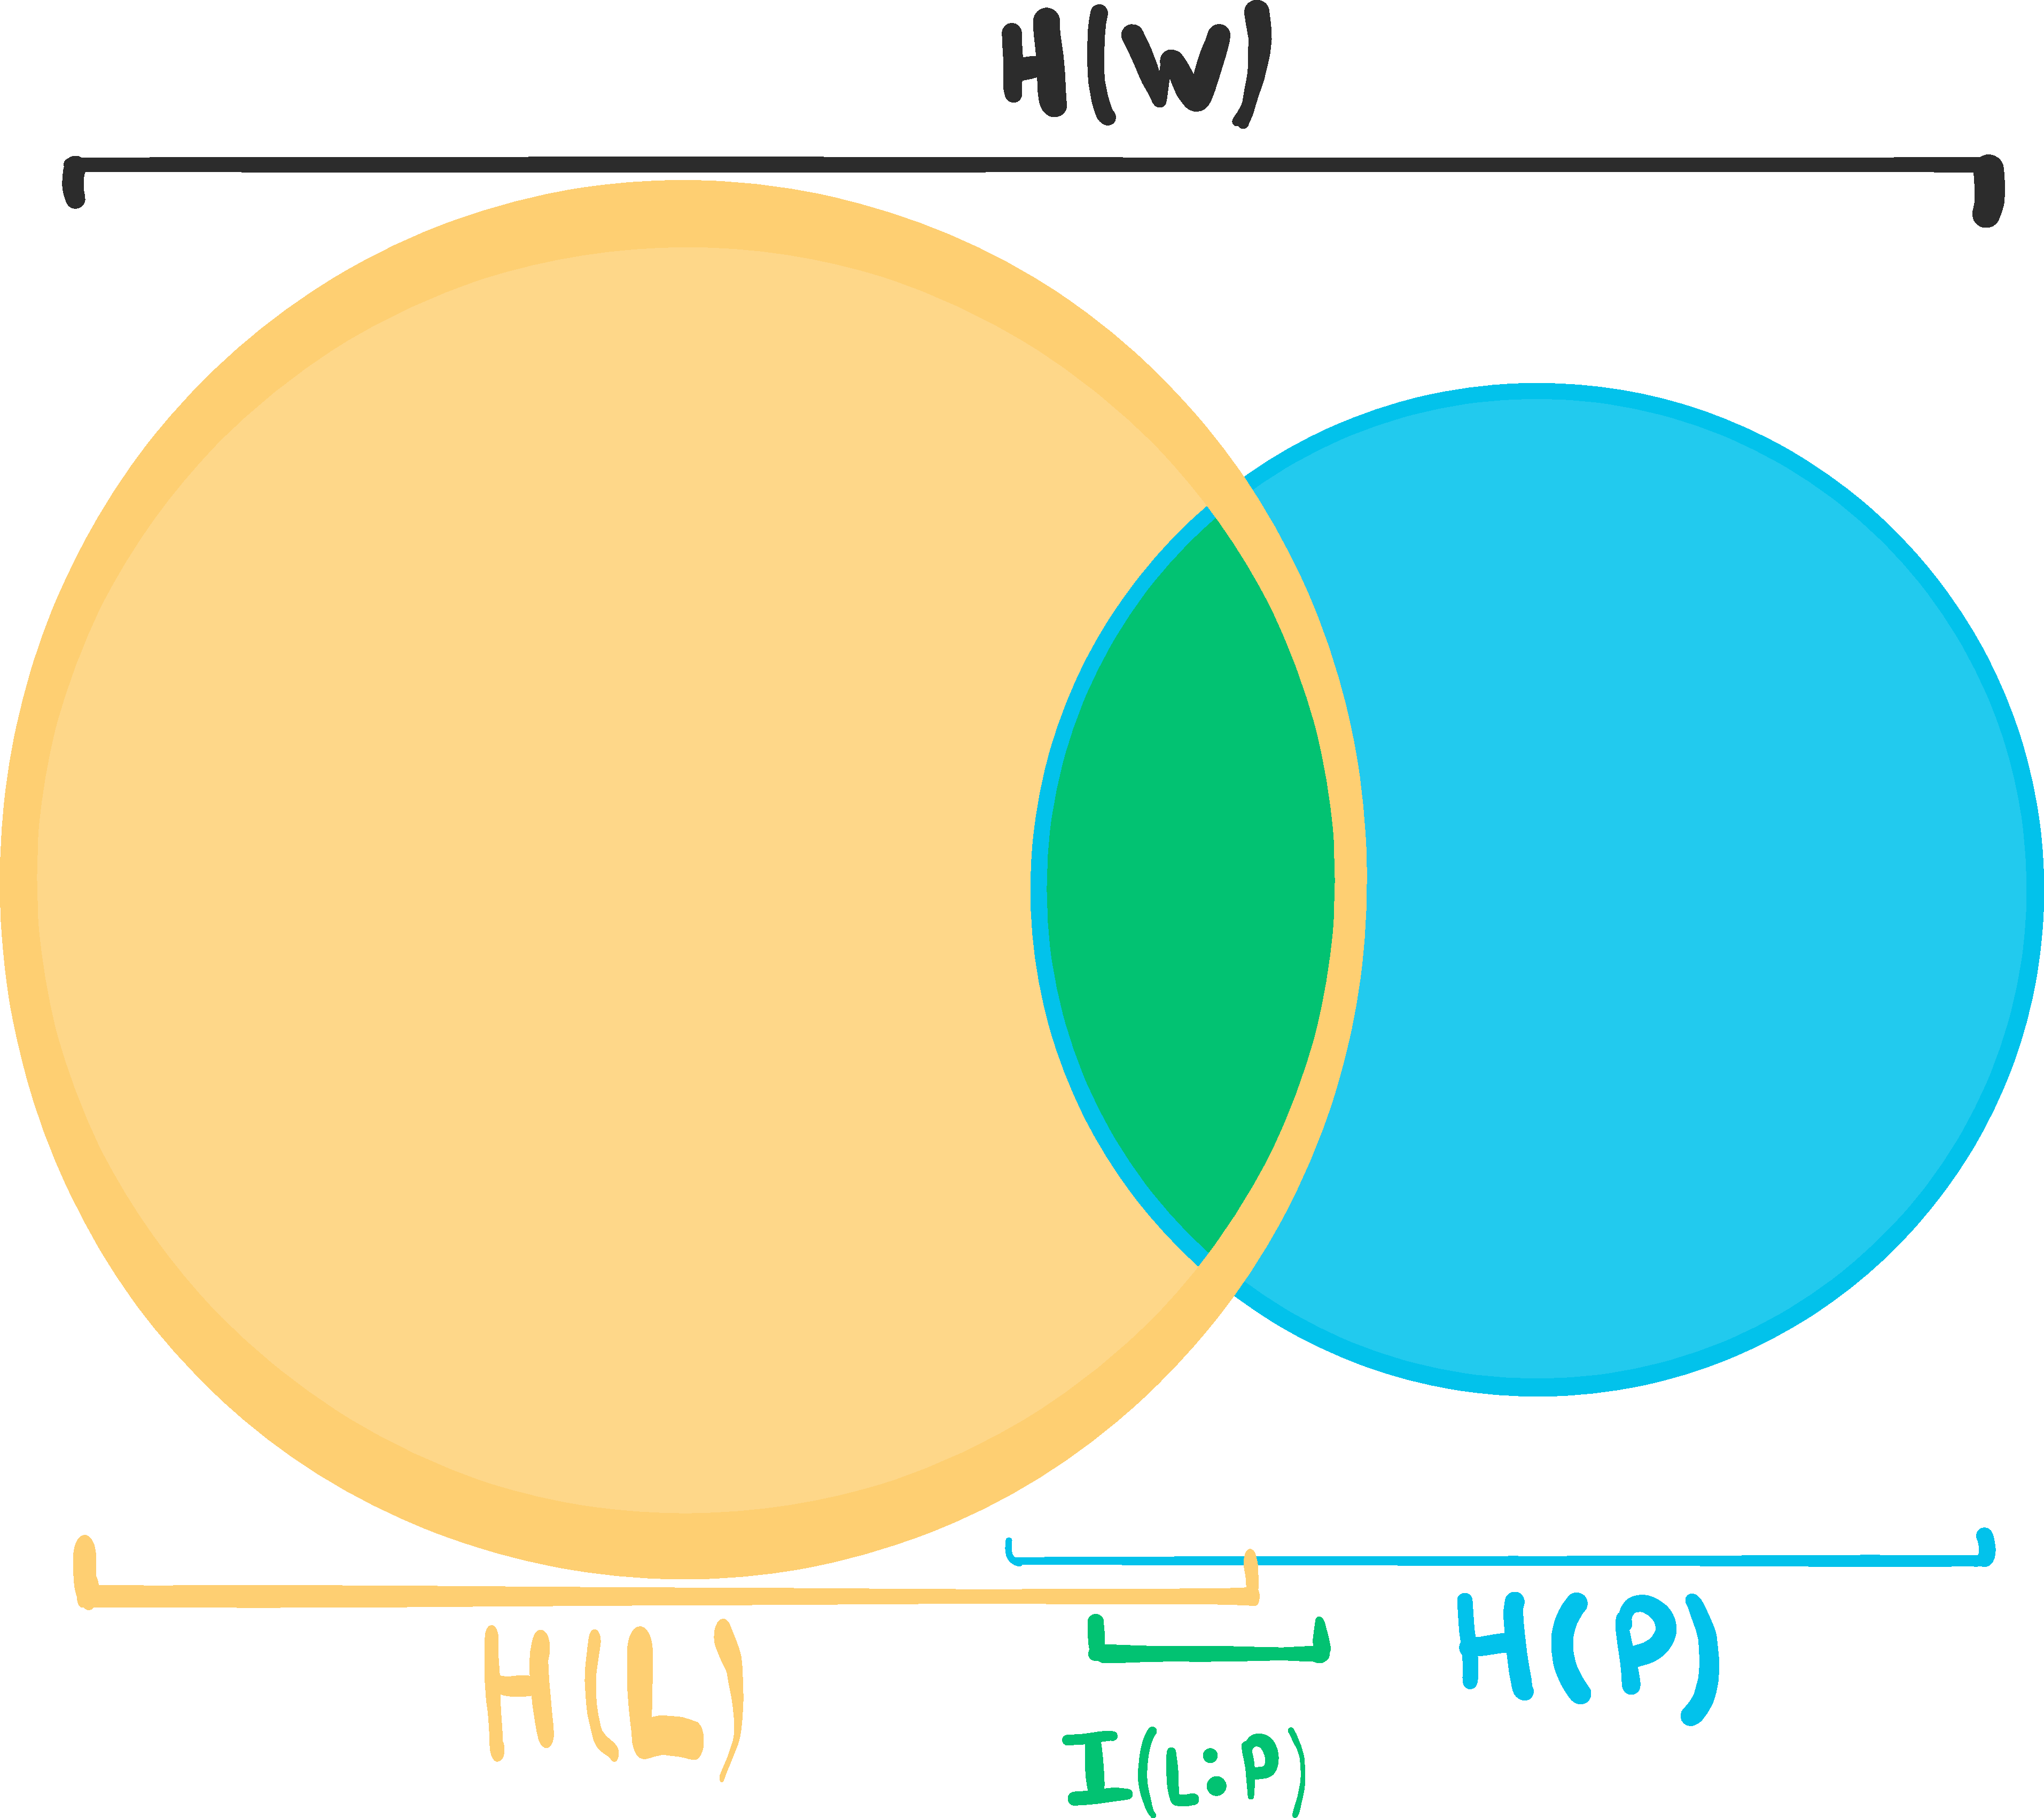
\includegraphics[trim= 0 0 0 0, clip, width=0.8\textwidth]{img/venn}
\end{center}
The green silver in the middle of this venn diagram is the entropy shared between $\bm{L}$ and $\bm{P}$.
I denoted that sliver $I( \bm{L} : \bm{P})$.
(Shared entropy is symmetric, so it would be just as valid to denote it $I( \bm{P} : \bm{L})$).
In total, the shaded area represents the entropy of the entire system $H(\bm{W})$.

This idea of sharing entropy has an interesting implication.
Say we had a rain meter that tells us the precipitation conditions.
Knowing the precipitation conditions removes all the blue uncertainty ($H(\bm{P})$) from our diagram, taking some of the yellow uncertainty ($H(\bm{L})$) with it.
\begin{center}
TODO
\end{center}
Thus, we would expect our uncertainty about light conditions to be reduced by knowing the precipitation conditions.
This is indeed the case.
We can calculate this directly!

To calculate the entropy after peeking at the rain meter, we need to calculate our uncertainty as to the light condition after we observe the rain meter.
There are two outcomes from looking at the rain meter --- we learn it's wet outside or we learn it's dry outside.
Remember the conditional probabilities we reviewed?
To calculate entropy given a particular precipitation state, we proceed as usual with Shannon's equation but substitute probabilities conditional on the precipitation state we observed for unconditional probabilities.

If we find it's wet outside, we calculate
\begin{align*}
H(\bm{L} | \bm{P} = \text{wet})
&=
- P(\bm{L} = \text{sunny} | \bm{P} = \text{wet}) \times \log_2(P(\bm{L} = \text{sunny} | \bm{P} = \text{wet})) \\
&+ - P(\bm{L} = \text{overcast} | \bm{P} = \text{wet}) \times \log_2(P(\bm{L} = \text{overcast} | \bm{P} = \text{wet})) \\
\approx&
- 0.05 \times \log_2(0.05) + - 0.95 \times \log_2(0.95) \\
\approx& 0.286.
\end{align*}
If we find it's dry outside, we calculate
\begin{align*}
H(\bm{L} | \bm{P} = \text{dry})
=&
- P(\bm{L} = \text{sunny} | \bm{P} = \text{dry}) \times \log_2(P(\bm{L} = \text{sunny} | \bm{P} = \text{dry})) \\
&+  - P(\bm{L} = \text{overcast} | \bm{P} = \text{dry}) \times \log_2(P(\bm{L} = \text{overcast} | \bm{P} = \text{dry})) \\
=&
- 0.55 \times \log_2(0.55) + - 0.45 \times \log_2(0.45) \\
\approx& 0.993.
\end{align*}

From these results, we can calculate the expected entropy of $\bm{L}$ given observation of $\bm{P}$.
We denote this quantity as $H(\bm{L}|\bm{P})$.
We calculate $H(\bm{L}|\bm{P})$ by taking an average of $H(\bm{L} | \bm{P} = \text{dry})$ and $H(\bm{L} | \bm{P} = \text{wet})$, weighted by the probabilities $P(\bm{P} = \text{wet})$ and $P(\bm{P} = \text{dry})$,
\begin{align*}
H(\bm{L} | \bm{P})
=&
P(\bm{P} = \text{wet}) \times H(\bm{L} | \bm{P} = \text{wet}) \\
&+ P(\bm{P} = \text{dry}) \times H(\bm{L} | \bm{P} = \text{dry}) \\
\approx& 0.1 \times [ - 0.05 \times \log_2(0.05) + - 0.95 \times \log_2(0.95) ] \\
&+ 0.9 \times [ - 0.55 \times \log_2(0.55) + - 0.45 \times \log_2(0.45) ] \\
\approx& 0.922.
\end{align*}

Recall that information is the difference between entropies.
Thus, we can think of the shared entropy between $\bm{P}$ and $\bm{L}$ as information gained with respect to $\bm{L}$ when we know the state of $\bm{P}$,
\begin{align*}
I(\bm{L} : \bm{P})
&=
H(\bm{L}) - H(\bm{L} | \bm{P}) \\
&\approx
1 - 0.922 \\
&\approx
0.078
\end{align*}
(This is why shared entropy is denoted with the capital $I$!)

The reverse holds true, as well.
Our uncertainty about light conditions is reduced by knowing the precipitation conditions.
Checking our light meter (instead of the rain meter) removes all the yellow uncertainty ($H(\bm{L})$) from our diagram, taking some of the blue uncertainty ($H(\bm{P})$) with it.
\begin{center}
TODO
\end{center}
Similar calculations give the expected entropy of $\bm{P}$ given observation of $\bm{L}$,
\begin{align*}
H(\bm{P} | \bm{L})
=&
P(\bm{L} = \text{overcast}) \times H(\bm{P} | \bm{L} = \text{overcast})
+ P(\bm{L} = \text{sunny}) \times H(\bm{P} | \bm{L} = \text{sunny}) \\
=&
P(\bm{L} = \text{overcast}) \times \Big[ - P(\bm{P} = \text{wet} | \bm{L} = \text{overcast}) \times \log_2(P(\bm{P} = \text{wet} | \bm{L} = \text{overcast})) \\
&+ - P(\bm{P} = \text{dry} | \bm{L} = \text{overcast}) \times \log_2(P(\bm{P} = \text{dry} | \bm{L} = \text{overcast})) \Big] \\
&+ P(\bm{L} = \text{sunny})\times \Big[ - P(\bm{P} = \text{wet} | \bm{L} = \text{sunny}) \times \log_2(P(\bm{P} = \text{wet} | \bm{L} = \text{sunny})) \\
&+ - P(\bm{P} = \text{dry} | \bm{L} = \text{sunny}) \times \log_2(P(\bm{P} = \text{dry} | \bm{L} = \text{sunny})) \Big] \\
=&
0.5 \times [ - 0.19 \times \log_2(0.19) + - 0.81 \times \log_2(0.81) ] \\
&+ 0.5 \times [ - 0.01 \times \log_2(0.01) + - 0.99 \times \log_2(0.99) ]
\approx&
0.391
\end{align*}

Thus, the information gained with respect to $\bm{P}$ when we know the state of $\bm{L}$ is
\begin{align*}
I(\bm{P} : \bm{L})
&=
H(\bm{P}) - H(\bm{P} | \bm{L}) \\
&\approx
0.469 - 0.391 \\
&\approx
0.078.
\end{align*}

We have computationally confirmed the symmetric nature of shared entropy,
\begin{align*}
I(\bm{L} : \bm{P})
&=
I(\bm{P} : \bm{L}) \\
0.078
&\stackrel{\checkmark}{\approx}
0.078
\end{align*}
Also, as we would expect from visual inspection of our Venn diagram of entropy,
\begin{align*}
H(\bm{W})
&=
H(\bm{P}) + H(\bm{L}) - I(\bm{L} : \bm{P}) \\
1.391
&\stackrel{\checkmark}{\approx}
0.469 + 1 - 0.078
\end{align*}


\section{Conclusion}

There you have it.
Information is the difference between entropies.
Entropy is a quantification of uncertainty.
If a discrete random variable models a situation, calculate entropy can be calculated as a function of the set of probabilities associated with the possible outcomes of the situation.
Just plug that set of probabilities into Shannon's equation to calculate entropy.

I hope these illustrated examples have helped you get a hands-on feel for information and entropy.
Now, go check out \cite{Adami2012} for some nicely described applications of information theory to biology and evolution.
If you want to further firm up your footing with information theory itself, give \cite{Adami2016} a read.
Don't be afraid to make your own toy problems and analyze them yourself!
It's the best way to get comfortable with any new math topic.

What's the entropy associated with a fair six-sided die?
What's the information content of a three letter code if all three letters are drawn independently from a uniform distribution over all 26 letters?
What if the three letters are drawn without replacement?
If you're looking for a challenge, maybe check out the \href{https://en.wikipedia.org/wiki/Monty_Hall_problem}{Monty Hall problem}.
What's the entropy when all three doors are closed?
What's the entropy after the host opens a goat door?
How much information is gained when the host opens a goat door?
This one's tricky.
Have fun!


\bibliography{bibl}
\bibliographystyle{apalike}

\end{document}
